% Para utilizar este template siga o tutorial disponível em http://www.biblioteca.ufc.br/wp-content/uploads/2015/09/tutorial-sharelatex.pdf

%%%%%%%%%%%%%%%%%%%%%%%%%%%%%%%%%%%%%%%%%%%%%%%%%%%%%%%
%% Você deve criar uma conta no Overleaf. Depois,    %%
%% vá nas opções no canto esquerdo superior da tela  %%
%% e clique em "Copiar Projeto". Dê um novo nome pa- %%
%% ra o projeto.                                     %%
%%                                                   %%
%% Os principais desenvolvedores deste template são: %%
%%                                                   %%
%%            Ednardo Moreira Rodrigues              %%
%%       (Doutor em Engenharia Elétrica - UFC)       %%
%%(Coord. do Grupo de Astronomia da Seara da Ciência)%%
%%                      &                            %%
%%            Alan Batista de Oliveira               %%
%%           (Engenheiro Eletricista - UFC)          %%
%%                                                   %%
%% Consultoria Bibliotecária                         %%
%%                                                   %%
%%  Versão 2016 - ShareLaTeX:                        %% 
%%                                                   %%
%% - Francisco Edvander Pires Santos;                %%
%% - Juliana Soares Lima;                            %%
%% - Izabel Lima dos Santos;                         %%
%% - Kalline Yasmin Soares Feitosa;                  %%
%% - Eliene Maria Vieira de Moura.                   %%
%% ------------------------------------------------- %% 
%%  Versão 2019,2020 - Overleaf:                     %%
%%                                                   %%
%%  Biblioteca de Ciências Humanas:                  %%
%% - Francisco Edvander Pires Santos;                %%
%% - Juliana Soares Lima;                            %%
%% - Eliene Maria Vieira de Moura;                   %%
%% - Edmundo Moreira de Sousa Filho.                 %%
%%                                                   %%
%% Biblioteca da FEAAC:                              %%
%% - Izabel Lima dos Santos;                         %%
%% - Kalline Yasmin Soares Feitosa;                  %%
%% - Kleber Lima dos Santos.                         %%
%%                                                   %%
%%  Biblioteca do Curso de Física:                   %%
%% - Aline Rodrigues de Lima Mendes;                 %%
%% - Maria de Jesus Silva dos Santos.                %%
%%                                                   %%
%%  Biblioteca Central do Campus do Pici:            %%
%% - Raquel da Silva Nascimento.                     %%
%% - Felipe Ferreira da Silva                        %%
%%  Versão 2019,2020 - Overleaf:                     %%
%%  ------------------------------------------------ %%
%%  Versão de 2022 - Overleaf                        %%
%%                                                   %%
%%   a) Felipe Ferreira da Silva                        %%
%%   b) Ednardo Moreira Rodrigues                       %%
%%   c) Comissão de Normalização do Sistema de          %%
%%      Bibliotecas da UFC                              %%
%%                                                   %%
%% Colaboradores                                     %%
%%                                                   %%
%% -Andrei Bosco Bezerra Torres                      %% 
%% (Professor - Sistemas e Mídias Digitais -         %%
%% Instituto Universidade Virtual - UFC)             %%
%% Tiago Alves Lima                                  %% 
%% (Aluno de Mestrado em Eng. Elétrica)              %%
%%                                                   %%
%% Grande parte do trabalho foi adaptado do template %%
%% da UECE elaborado por:                            %%
%% Thiago Nascimento  (UECE)                         %%
%% Project available on:                             %%
%% https://github.com/thiagodnf/uecetex2             %%
%%                                                   %%
%% "Dúvidas, esclarecimentos ou sugestões podem ser  %%
%% enviadas para o seguinte e-mail:                  %%
%%                                                   %%
%%             bu@ufc.br               %%
%%                                                   %%
%% As últimas atualizações estão descritas no inicio %%
%% do arquivo "README.md".                           %%
%%                                                   %%
%%%%%%%%%%%%%%%%%%%%%%%%%%%%%%%%%%%%%%%%%%%%%%%%%%%%%%%

\documentclass[        
    a4paper,          % Tamanho da folha A4
    12pt,             % Tamanho da fonte 12pt
    chapter=TITLE,    % Todos os capitulos devem ter caixa alta
    section=Title,    % Todas as secoes devem ter caixa alta somente na primeira letra
    subsection=Title, % Todas as subsecoes devem ter caixa alta somente na primeira letra
    oneside,          % Usada para impressao em apenas uma face do papel
    english,          % Hifenizacoes em ingles
    spanish,          % Hifenizacoes em espanhol
    brazil,           % Ultimo idioma eh o idioma padrao do documento
    fleqn             % Comente esta linha se quiser centralizar as equacoes. Comente também a linha 65 abaixo
]{lib/abntex2}

% Para utilizar este template siga o tutorial disponível em http://www.biblioteca.ufc.br/wp-content/uploads/2015/09/tutorial-sharelatex.pdf

%%%%%%%%%%%%%%%%%%%%%%%%%%%%%%%%%%%%%%%%%%%%%%%%%%%%%%%
%% Você deve criar uma conta no Overleaf. Depois,    %%
%% vá nas opções no canto esquerdo superior da tela  %%
%% e clique em "Copiar Projeto". Dê um novo nome pa- %%
%% ra o projeto.                                     %%
%%                                                   %%
%% Os principais desenvolvedores deste template são: %%
%%                                                   %%
%%            Ednardo Moreira Rodrigues              %%
%%       (Doutor em Engenharia Elétrica - UFC)       %%
%%(Coord. do Grupo de Astronomia da Seara da Ciência)%%
%%                      &                            %%
%%            Alan Batista de Oliveira               %%
%%           (Engenheiro Eletricista - UFC)          %%
%%                                                   %%
%% Consultoria Bibliotecária                         %%
%%                                                   %%
%%  Versão 2016 - ShareLaTeX:                        %% 
%%                                                   %%
%% - Francisco Edvander Pires Santos;                %%
%% - Juliana Soares Lima;                            %%
%% - Izabel Lima dos Santos;                         %%
%% - Kalline Yasmin Soares Feitosa;                  %%
%% - Eliene Maria Vieira de Moura.                   %%
%%                                                   %% 
%%  Versão 2019 - Overleaf:                          %%
%%                                                   %%
%%  Biblioteca de Ciências Humanas:                  %%
%% - Francisco Edvander Pires Santos;                %%
%% - Juliana Soares Lima;                            %%
%% - Eliene Maria Vieira de Moura;                   %%
%% - Edmundo Moreira de Sousa Filho.                 %%
%%                                                   %%
%% Biblioteca da FEAAC:                              %%
%% - Izabel Lima dos Santos;                         %%
%% - Kalline Yasmin Soares Feitosa;                  %%
%% - Kleber Lima dos Santos.                         %%
%%                                                   %%
%%  Biblioteca do Curso de Física:                   %%
%% - Aline Rodrigues de Lima Mendes;                 %%
%% - Maria de Jesus Silva dos Santos.                %%
%%                                                   %%
%%  Biblioteca Central do Campus do Pici:            %%
%% - Raquel da Silva Nascimento.                     %%
%% - Felipe Ferreira da Silva                        %%
%%                                                   %%
%% Colaboradores                                     %%
%%                                                   %%
%% -Andrei Bosco Bezerra Torres                      %% 
%% (Professor - Sistemas e Mídias Digitais -         %%
%% Instituto Universidade Virtual - UFC)             %%
%% Tiago Alves Lima                                  %% 
%% (Aluno de Mestrado em Eng. Elétrica)              %%
%%                                                   %%
%% Grande parte do trabalho foi adaptado do template %%
%% da UECE elaborado por:                            %%
%% Thiago Nascimento  (UECE)                         %%
%% Project available on:                             %%
%% https://github.com/thiagodnf/uecetex2             %%
%%                                                   %%
%% "Dúvidas, esclarecimentos ou sugestões podem ser  %%
%% enviadas para o seguinte e-mail:                  %%
%%                                                   %%
%%             atendimentobch@ufc.br                 %%
%%                                                   %%
%% As últimas atualizações estão descritas no inicio %%
%% do arquivo "README.md".                           %%
%%                                                   %%
%%%%%%%%%%%%%%%%%%%%%%%%%%%%%%%%%%%%%%%%%%%%%%%%%%%%%%%

% Importações de pacotes
\usepackage[utf8]{inputenc}                         % Acentuação direta
\usepackage[T1]{fontenc}                            % Codificação da fonte em 8 bits
\usepackage{graphicx}                               % Inserir figuras
\usepackage{amsfonts, amssymb, amsmath}             % Fonte e símbolos matemáticos
\usepackage{booktabs}                               % Comandos para tabelas
\usepackage{verbatim}                               % Texto é interpretado como escrito no documento
\usepackage{multirow, array}                        % Múltiplas linhas e colunas em tabelas
\usepackage{indentfirst}                            % Endenta o primeiro parágrafo de cada seção.
\usepackage{listings}                               % Utilizar codigo fonte no documento
\usepackage{xcolor}
\usepackage{microtype}                              % Para melhorias de justificação?
%PIF17042024
%\usepackage[portuguese,ruled,lined,linesnumbered]{algorithm2e}    % Escrever algoritmos
\usepackage[portuguese,portuguesekw,ruled,lined,linesnumbered]{algorithm2e}    % Escrever algoritmos
%\usepackage{algorithmic}                            % Criar Algoritmos  
%\usepackage{float}                                 % Utilizado para criação de floats
\usepackage{amsgen}
\usepackage{lipsum}                                 % Usar a simulação de texto Lorem Ipsum
%\usepackage{titlesec}                              % Permite alterar os títulos do documento
\usepackage{tocloft}                                % Permite alterar a formatação do Sumário
\usepackage{etoolbox}                               % Usado para alterar a fonte da Section no Sumário
\usepackage[nogroupskip,nonumberlist]{glossaries}   % Permite fazer o glossario. A apcao "sort=use" faz com que as siglas aparecam na lista conformse sao usadas no texto.

\usepackage[format=plain,justification=justified,skip=0pt,singlelinecheck = false,labelsep=colon]{caption}            % Altera o comportamento da tag caption. Algumas opcoes do caption so podem ser alternada no arquivo "antex2.cls, linhas 334 a 348.

\usepackage[alf, abnt-emphasize=bf, recuo=0cm, abnt-etal-cite=2, abnt-etal-list=0, abnt-etal-text=it]{lib/ufcTexcite}  % Citações padrão UFC/ABNT NBR 6023 de 2018
%\usepackage[bottom]{footmisc}                      % Mantém as notas de rodapé sempre na mesma posição
%\usepackage{times}                                 % Usa a fonte Times
%%%%%%%%%%%%%%%%%%% AVISO %%%%%%%%%%%%%%%%%%%%%%%%%%%%%%%%%%%%%%%%
%descomente as duas linhas abaixo para alterar o texto de Times New Roman para Arial:

%\usepackage{helvet}
%\renewcommand{\familydefault}{\sfdefault}  % Usa a fonte Arial              
%%%%%%%%%%%%%%%%%%%%%%%%%%%%%%%%%%%%%%%%%%%%%%%%%%%%%%%%%%%%%%%%%%

\usepackage{mathptmx}         % Usa a fonte Times New Roman			%\usepackage{lmodern}         % Usa a fonte Latin Modern
%\usepackage{subfig}          % Posicionamento de figuras
%\usepackage{scalefnt}        % Permite redimensionar tamanho da fonte
%\usepackage{color, colortbl} % Comandos de cores
%\usepackage{lscape}          % Permite páginas em modo "paisagem"
%\usepackage{ae, aecompl}     % Fontes de alta qualidade
%\usepackage{picinpar}        % Dispor imagens em parágrafos
%\usepackage{latexsym}        % Símbolos matemáticos
%\usepackage{upgreek}         % Fonte letras gregas
\usepackage{appendix}         % Gerar o apendice no final do documento
\usepackage{paracol}          % Criar paragrafos sem identacao
\usepackage{lib/ufcTex}	      % Biblioteca com as normas da UFC para trabalhos academicos
\usepackage{pdfpages}         % Incluir pdf no documento
\usepackage{amsmath}          % Usar equacoes matematicas

\makeglossaries % Organiza e gera a lista de abreviaturas, simbolos e glossario
\makeindex      % Gera o Indice do documento         

\renewcommand{\labelitemi}{\textendash} %Altera os marcadores de itemize para 





\setlength{\mathindent}{0pt} %Complementa o alinhamento de equações para totalmente a esquerda.
\usepackage[utf8]{inputenc}
\usepackage{import}
\usepackage{color, colortbl}
\usepackage{tikz}
\usepackage[brazil]{babel}
%PIF05102023: resolve problemas com hyphenation
\usepackage[T1]{fontenc}
\usepackage{verbatim}
\usepackage{amsfonts}
\usepackage{multicol}
\usepackage{euscript}
\usepackage{float}
\usepackage{multirow}
\usepackage{array}
\usepackage{rotating}
\usepackage{amsmath}
\usepackage{tikz,tkz-euclide}
\usetikzlibrary{arrows,calc,patterns}
\usepackage{epsfig,graphicx,cite}
\usepackage{array}
\newcolumntype{P}[1]{>{\centering\arraybackslash}p{#1}}

\definecolor{ninfect}{HTML}{457b9d}
\definecolor{infect}{HTML}{d62828}
\definecolor{border}{HTML}{1d2a34}
\definecolor{ninteract}{HTML}{2a9d8f}
\definecolor{azuul}{HTML}{2b4c28}
\usetikzlibrary[shadows]
\usetikzlibrary{arrows,calc,patterns}
\definecolor{Gray}{gray}{0.9}

\usepackage{mathrsfs}
% Use o bibtex
\newcommand{\mycomment}[1]{}
\usetikzlibrary{calc}
\tikzset{make origin horizontal center of bounding box/.style={%
execute at end picture={%
\path let \p1=(current bounding box.west),\p2=(current bounding box.east)
in ({-max(-1*\x1,\x2)},\y1) ({max(-1*\x1,\x2)},\y1);
}}}
\DeclareMathAlphabet{\mathpzc}{OT1}{pzc}{m}{it}
\usepackage{lineno}
\usepackage{anyfontsize} %PIF15042024


%%%%%%%%%%%%%%%%%%%%%%%%%%%%%%%%%%%%%%%%%%%%%%%%%%%%%
%%                     ATENCAO                     %%
%%%%%%%%%%%%%%%%%%%%%%%%%%%%%%%%%%%%%%%%%%%%%%%%%%%%%
%  Qual e o nivel do trabalho academico que voce esta 
% escrevendo? Retire o simbolo "%" apenas de um dos 
% quatro topicos abaixo refente ao nível do seu traba
% -lho.

%\trabalhoacademico{tccgraduacao}
%\trabalhoacademico{tccespecializacao}
\trabalhoacademico{dissertacao}
%\trabalhoacademico{tese}

%%%%%%%%%%%%%%%%%%%%%%%%%%%%%%%%%%%%%%%%%%%%%%%%%%%%%

% Define se o trabalho e uma qualificacao
% Coloque 'nao' para versao final do trabalho

\ehqualificacao{nao}

% Remove as bordas vermelhas e verdes do PDF gerado
% Coloque 'sim' pare remover

\removerbordasdohyperlink{sim} 

% Adiciona a cor Azul a todos os hyperlinks

\cordohyperlink{nao}

%%%%%%%%%%%%%%%%%%%%%%%%%%%%%%%%%%%%%%%%%%%%%%%%%%%%%
%%         Informacao sobre a instituicao          %%
%%%%%%%%%%%%%%%%%%%%%%%%%%%%%%%%%%%%%%%%%%%%%%%%%%%%%

\ies{Universidade Federal do Ceará}
\iessigla{UFC}
\centro{Centro de Ciências}
\departamento{Departamento de ESTATÍSTICA E MATEMÁTICA APLICADA}

%%%%%%%%%%%%%%%%%%%%%%%%%%%%%%%%%%%%%%%%%%%%%%%%%%%%%
%%        Informacao para TCC de Graduacao         %%
%%%%%%%%%%%%%%%%%%%%%%%%%%%%%%%%%%%%%%%%%%%%%%%%%%%%%

\graduacaoem{Engenharia Xxxxxxx}
\habilitacao{bacharel} % Ou licenciado(a)

% AVISO: Caso necessario alterar o texto de apresenta-
% cao da Especializacao, ir a pasta "lib", arquivo 
% "ufctex.sty" na linha 502.


%%%%%%%%%%%%%%%%%%%%%%%%%%%%%%%%%%%%%%%%%%%%%%%%%%%%%
%%     Informacao para TCC de Especializacao       %%
%%%%%%%%%%%%%%%%%%%%%%%%%%%%%%%%%%%%%%%%%%%%%%%%%%%%%

\especializacaoem{Yyyyyyyyy}

% AVISO: Caso necessario alterar o texto de apresenta-
% cao da Especializacao, ir a pasta "lib", arquivo 
% "ufctex.sty" na linha 507.

%%%%%%%%%%%%%%%%%%%%%%%%%%%%%%%%%%%%%%%%%%%%%%%%%%%%%
%%         Informacao para Dissertacao             %%
%%%%%%%%%%%%%%%%%%%%%%%%%%%%%%%%%%%%%%%%%%%%%%%%%%%%%

\programamestrado{Programa de Pós-Graduação em Modelagem e Métodos Quantitativos}
%\nomedomestrado{Mestrado Acadêmico em Modelagem e Métodos Quantitativos}
\mestreem{Modelagem e Métodos Quantitativos}
\areadeconcentracaomestrado{Modelagem e Métodos Quantitativos}

% AVISO: Caso necessario alterar o texto de apresenta-
% cao da dissertacao, ir a pasta "lib", arquivo 
% "ufctex.sty" na linha 511.

%%%%%%%%%%%%%%%%%%%%%%%%%%%%%%%%%%%%%%%%%%%%%%%%%%%%%
%%               Informação para Tese              %%
%%%%%%%%%%%%%%%%%%%%%%%%%%%%%%%%%%%%%%%%%%%%%%%%%%%%%

\programadoutorado{Programa de Pós-Graduação em Xxxxxx}
\nomedodoutorado{Doutorado em Xxxxxxx}
\doutorem{Engenharia Xxxxxx}
\areadeconcentracaodoutorado{Engenharia Xxxxxxx}

% AVISO: Caso necessario alterar o texto de apresenta-
% cao da tese, ir a pasta "lib", arquivo "ufctex.sty" 
% na linha 515.

%%%%%%%%%%%%%%%%%%%%%%%%%%%%%%%%%%%%%%%%%%%%%%%%%%%%%
%%      Informacoes relacionadas ao trabalho       %%
%%%%%%%%%%%%%%%%%%%%%%%%%%%%%%%%%%%%%%%%%%%%%%%%%%%%%

\autor{Carlos Miguel Moreira Gonçalves}
\titulo{Estratégias de Vacinação em Redes Complexas}
\data{2024}
\local{Fortaleza}

% Exemplo: \dataaprovacao{01 de Janeiro de 2012}
\dataaprovacao{xx/xx/xxxx.}

%%%%%%%%%%%%%%%%%%%%%%%%%%%%%%%%%%%%%%%%%%%%%%%%%%%%%
%%           Informação sobre o Orientador         %%
%%%%%%%%%%%%%%%%%%%%%%%%%%%%%%%%%%%%%%%%%%%%%%%%%%%%%

\orientador{Prof. Dr. Leandro Chaves Rêgo}
\orientadories{Universidade Federal do Ceará (UFC)}
\orientadorcentro{Centro de Ciências(CC)}
\orientadorfeminino{nao} % Coloque 'sim' se for do sexo feminino

%%%%%%%%%%%%%%%%%%%%%%%%%%%%%%%%%%%%%%%%%%%%%%%%%%%%%
%%          Informação sobre o Coorientador        %%
%%%%%%%%%%%%%%%%%%%%%%%%%%%%%%%%%%%%%%%%%%%%%%%%%%%%%

% Deixe o nome do coorientador em branco para remover do documento

\coorientador{Prof. Dr.  Pablo Ignacio Fierens}
\coorientadories{Instituto Tecnológico de Buenos Aires (ITBA)}
\coorientadorcentro{Centro do Coorientador (SIGLA)}
\coorientadorfeminino{nao} % Coloque 'sim' se for do sexo feminino

%%%%%%%%%%%%%%%%%%%%%%%%%%%%%%%%%%%%%%%%%%%%%%%%%%%%%
%%              Informação sobre a banca           %%
%%%%%%%%%%%%%%%%%%%%%%%%%%%%%%%%%%%%%%%%%%%%%%%%%%%%%

% Atenção! Deixe em branco o nome do membro da banca para remover da folha de aprovacao

% Exemplo de uso:
% \membrodabancadois{Prof. Dr. Fulano de Tal}
% \membrodabancadoisies{Universidade Federal do Ceará - UFC}


\membrodabancadois{Prof. Dr. Xxxxxxx Xxxxxx Xxxxxxx}
\membrodabancadoiscentro{Faculdade de Filosofia Dom Aureliano Matos (FAFIDAM)}
\membrodabancadoisies{Universidade do Membro da Banca três (SIGLA)}
\membrodabancatres{Prof. Dr. Xxxxxxx Xxxxxx Xxxxxxx}
\membrodabancatrescentro{Centro de Ciências e Tecnologia (CCT)}
\membrodabancatresies{Universidade do Membro da Banca quatro (SIGLA)}
\membrodabancaquatro{Prof. Dr. Xxxxxxx Xxxxxx Xxxxxxx}
\membrodabancaquatrocentro{Centro de Ciências e Tecnologia (CCT)}
\membrodabancaquatroies{Universidade do Membro da Banca cinco (SIGLA)}
\membrodabancacinco{Prof. Dr. Xxxxxxx Xxxxxx Xxxxxxx}
\membrodabancacincocentro{Teste}
\membrodabancacincoies{Universidade do Membro da Banca seis (SIGLA)}
\membrodabancaseis{Prof. Dr. Xxxxxxx Xxxxxx Xxxxxxx}
\membrodabancaseiscentro{}
\membrodabancaseisies{Universidade do Membro da Banca sete (SIGLA)}

\begin{document}	
	% Elementos pré-textuais
       % \imprimircapa{}
 
	% \imprimirfolhaderosto{}
	% \imprimirfichacatalografica{1-pre-textuais/ficha-catalografica}
	% %\imprimirerrata{elementos-pre-textuais/errata}
	% \imprimirfolhadeaprovacao
	% \imprimirdedicatoria{1-pre-textuais/dedicatoria}
	% \imprimiragradecimentos{1-pre-textuais/agradecimentos}
	% \imprimirepigrafe{1-pre-textuais/epigrafe}
	%\imprimirresumo{1-pre-textuais/resumo}
	%\imprimirabstract{1-pre-textuais/abstract}
	\renewcommand*\listfigurename{Lista de Figuras} %Se você comentar esta linha o título da lista fica: LISTA DE ILUSTRAÇÕES
	%\imprimirlistadeilustracoes
	%\imprimirlistadetabelas
	%\imprimirlistadequadros
	%\imprimirlistadealgoritmos
	%\imprimirlistadecodigosfonte
	%\imprimirlistadeabreviaturasesiglas
	%\imprimirlistadesimbolos{1-pre-textuais/lista-de-simbolos}   
	%\imprimirsumario
	
	\setcounter{table}{0}% Deixe este comando antes da primeira tabela.
	
	%Elementos textuais
	\textual
	%\chapter{Introdução}
Desde as mais antigas civilizações humanas, elas têm enfrentado o problema de propagação de doenças em larga escala~\cite{historic}. 
Por exemplo, em 
430 a.C. aconteceu a epidemia chamada Peste de Atenas que foi responsável pela morte de cerca de 
um terço  da população dessa cidade, em 
541 houve a primeira pandemia chamada Praga de Justiniano que ocorreu no mediterrâneo, 
e 
em 1347 aconteceu a mais devastadora pandemia na história da humanidade, a Peste Negra. Mais recentemente tivemos a Gripe Suína em 2009 e recentemente a Covid-19 e a Sétima Pandemia da Cólera. Nesse sentido, o estudo de 
doenças se tornou cada vez mais necessário para cientistas seja para entender como uma 
doença afeta o nosso corpo, seja para modelar a propagação dela.

Outrossim, com a expansão da humanidade nos últimos anos a partir do comércio, desmatamento e turismo facilitou a interação entre humanos e entre humanos e animais. Isso favoreceu uma maior propagação de doenças entre os países~\cite{area}. Essa propagação tem 4 classificações possíveis de acordo com a taxa de contágio e a sua área de atuação~\cite{whats}:

\begin{itemize}
  \item \textbf{Endemia} significa que uma infecção tem taxa de contágio controlada e previsível que atua desde uma cidade até um continente tem caráter contínuo e restrito a uma área geográfica ou população;
  \item \textbf{Surto} expressa um aumento repentino na ocorrência de casos da doença em pequenas áreas;
  \item \textbf{Epidemia} é um surto em grande escala;
  \item \textbf{Pandemia} é uma epidemia em escala mundial.
\end{itemize}

Dessa forma, a busca pelo entendimento das doenças emergiu como uma necessidade primordial desde os tempos mais remotos da história humana. Esse impulso de compreensão deu origem ao campo da Epidemiologia, uma disciplina voltada para a análise quantitativa e qualitativa dessas enfermidades. Essa área tem início com os estudos de Hipócrates~\cite{epidemiologia01} sobre como o ambiente 
favorece ou dificulta o surgimento de doenças. Apesar disso, foi apenas no século XIX que ganhou mais força com John Snow no estudo sobre a cólera em Londres. 
Snow descobriu que as mortes de cólera de 1848-49 e 1853-54 estavam relacionadas à água que os enfermos tomavam que era fornecida pela companhia Southpark. Outrossim, em 1760 Daniel Bernoulli foi o primeiro a tentar modelar 
matematicamente a propagação de doenças 
e as consequências da vacinação ~\cite{bernoulli2004attempt,Dietz2002}.
Já no século XX, os modelos compartimentais de transmissão de doenças foram introduzidos~\cite{kermack1927contribution} e 
 Richard Doll e Andrew Hill que descobriram a relação entre fumar e desenvolvimento de câncer~\cite{Doll1950}. 

Desde então a matemática mostrou-se cada vez mais essencial para estudo de doenças não apenas pela análise de dados, mas também na modelagem, pois não é eticamente correto fazer experimentações utilizando doenças, principalmente em humanos, então modelar matematicamente se torna essencial para previsões de propagação. Ademais, o entendimento da biologia por trás também é necessário para ter um modelo mais verossímil e seus resultados tenham 
validação na realidade.
Por fim, todo o conhecimento construído até aqui foi essencial para o entendimento e previsão da pandemia do novo Corona-vírus que durou de 11 de março de 2020 até 5 de maio de 2023.

\section{Covid-19}

Em dezembro de 2019, alguns casos de uma pneumonia de causas desconhecidas surgiram em Wuhan, capital da província de Hubei, um grande centro de transporte da China~\cite{Singhal2020}. 
Os pacientes que apresentaram esses sintomas faziam parte de um mercado de animais marinhos. Autoridades de saúde da China foram acionadas e foram coletadas amostras do patógeno para investigação 
e 
para caracterizar e controlar o desconhecido patógeno. No dia 31 de dezembro, o país notificou a OMS sobre o surto da doença e no dia seguinte o mercado da região foi fechado. No dia 7 de janeiro, cientistas conseguiram isolar o agente infecioso~\cite{Wang2020} e foi identificado com mais de 95\% de semelhança com o coronavírus apresentado em morcegos e mais de 70\% com SARS-CoV. No dia 23 de janeiro, já havia casos espalhados em 32 províncias da China e no mesmo dia toda a população de Wuhan foi colocada em \textit{lockdown}. Contudo, dois dias depois aconteceria a comemoração do Ano Novo Chinês e várias pessoas de outros países haviam viajado com intuito de participar do evento. No dia 11 de março, a OMS declara emergência de saúde pública do chamado Coronavírus ou COVID-19 e somente em
5 de maio de 2023 deixa de se tornar uma ameaça global.

Para evitar a proliferação do vírus, várias políticas públicas 
foram implementadas em todo o mundo. Estas políticas incluíam restrições de mobilidade, como \textit{lockdowns} e quarentenas, a fim de reduzir a interação social e a transmissão do vírus. Além disso, a promoção do uso de máscaras faciais, a intensificação da testagem e rastreamento de contatos, bem como a implementação de medidas de distanciamento físico em ambientes públicos, foram amplamente adotadas~\cite{PalaciosCruz2021}. 

No entanto, a centralização nas políticas de distanciamento social, que impuseram a necessidade de confinamento domiciliar à população, deu origem a desafios de natureza econômica~\cite{Irawan2021}. Isso se deveu, em grande parte, à impossibilidade de uma parcela substancial da força de trabalho desempenhar suas funções, resultando em um aumento significativo nas taxas de desemprego e na deterioração das condições sociais, com notável impacto negativo na qualidade da educação~\cite{10.1371/journal.pone.0239490}. O fechamento de instituições de ensino, como escolas e universidades, que são locais propensos a grandes aglomerações, agravou ainda mais essas questões. Como resultado desse contexto complexo, emergiu uma preocupação crítica com a saúde mental~\cite{Pereira2020}.


Devido a isso a campanha de vacinação em massa também se tornou uma política crucial para o fim da pandemia e minimizar 
o impacto dela 
na saúde pública e na economia. Um dos principais desafios da vacinação é a complexidade do processo de fabricação, que requer instalações especializadas, reagentes e tecnologia de ponta. Além disso, a demanda mundial por vacinas tem sobrecarregado a capacidade de produção existente, levando a atrasos na entrega de doses. A logística de distribuição também é complicada, com necessidade de armazenamento em temperaturas específicas para algumas vacinas, o que requer infraestrutura adequada. A obtenção de matérias-primas e ingredientes essenciais pode ser afetada por interrupções na cadeia de suprimentos global, causando a escassez de insumos.

\section{Estado da Arte}

Paralelamente aos avanços na prevenção da pandemia, houve um considerável aprimoramento dos modelos epidemiológicos, resultando em mais sofisticados e especializados na compreensão da propagação de doenças infecciosas~\cite{Xiang2021}. Esses modelos têm sido essenciais para orientar estratégias de controle da COVID-19, incluindo a implementação de programas de vacinação~\cite{Scabini2021, BustamanteCastaeda2021, Loyal2020}. No entanto, é importante observar que os modelos epidemiológicos tradicionais, embora sejam valiosos para prever tendências em larga escala, podem não capturar detalhes específicos das interações locais e complexas que ocorrem em estruturas de rede~\cite{Pellis2015}.

Os modelos epidemiológicos baseados em redes representam uma abordagem que enfatiza a análise das interações individuais em sistemas complexos, buscando compreender a propagação de doenças em escalas locais e com detalhes de rede. Esses modelos consideram a estrutura da rede, que descreve as conexões interpessoais e os contatos sociais, e incorporam processos de transmissão de doenças em estruturas de rede realistas~\cite{Pei2023}. \citeonline{pastor2002immunization,eames2003contact} utilizam o modelo de redes com propriedades de pequeno mundo para estudar a imunização e encontram expoentes críticos para a evolução da infecção. Enquanto que \citeonline{salathe2010dynamics,kitsak2010identification,Gong2013,miller2007effective} estudam formas de encontrar os sítios centrais na propagação das doenças utilizando algumas métricas de redes.


No entanto, é relevante destacar que essa abordagem ainda não incorporou completamente os avanços em complexidade ~\cite{Eikenberry2020} alcançados pelos modelos epidemiológicos 
que não utilizam informações de contatos ~\cite{Pellis2015}. Esses avanços estão relacionados à uma maior especialização em relação a doença com a introdução de novos componentes relevantes, como a distinção entre os sintomáticos e os assintomáticos, além de considerar aspectos relacionados à reação da sociedade, como a implementação de medidas de quarentena.

Entretanto os modelos de redes têm avançado por outras frentes como por exemplo a vacinação de uma população de uma mesma doença com cepas diferentes~\cite{Li2023}, em estudo na qual a população se adapta à propagação da doença se utilizando de isolamento ~\citeonline{Silva2023} estudam em redes com distribuição de grau em lei de potência e aplicando a teoria de campo médio para prever o comportamento da epidemia, em estudo da importância de viagens entre cidades~\cite{Quiroga2023,DellaRossa2020}, do transporte~\cite{Scabini2021}, distanciamento social~\cite{Maheshwari2020} e agrupamento~\cite{Craig2020} para o espalhamento da doença. Além disso, ainda no que tange COVID e vacinação existem estudos utilizando redes e modelos de infecção para estudar o espalhamento da aceitação ou não aceitação da vacinação~\cite{n_vacina}.

Esses estudos sobre a COVID-19 têm explorado diversas abordagens para entender a dinâmica da pandemia, desde a previsão de curvas de infecção~\cite{Xiang2021} até a avaliação de estratégias de intervenção~\cite{Liu2022,kitsak2010identification}, como distanciamento social, \textit{lockdowns} e, principalmente, campanhas de vacinação. Através da análise de eficácia, cobertura vacinal e estratégias de implementação, é possível avaliar o impacto das vacinações em larga escala na redução da transmissão de patógenos e na proteção da saúde da população. Além disso, esses estudos contribuem para a tomada de decisões informadas sobre quais vacinas priorizar, quais grupos populacionais devem ser alvo e como otimizar recursos limitados. O estudo de estratégias de vacinação para COVID-19 não é novidade na literatura, ~\cite{Doostmohammadian2020,Tetteh2021,Chen2022,Petrizzelli2022}, entretanto os estudos estavam limitados a: redes tradicionais com pouca base no real, modelos epidemiológicos pouco especializados com a doença, sem levar consideração a idade do indivíduo ou tempo de contato entre eles e ou estudo de poucas métricas de centralidade.


\section{Descrição do Problema}

A incorporação de modelos epidemiológicos robustos em conjunto com a modelagem de redes, considerando a estratificação etária, representa um desenvolvimento metodológico que, em grande parte, não havia sido abordado satisfatoriamente na literatura. Essa abordagem combinada possibilita uma análise mais precisa e abrangente das interações sociais e da disseminação de doenças, levando em conta as diferenças demográficas relacionadas à idade. Ao fazer isso, abrem-se oportunidades para melhorar a modelagem de surtos epidêmicos e a eficácia das estratégias de intervenção, com foco na melhoria da vacinação em grupos etários específicos.


Vale ressaltar que, historicamente, a identificação de nós centrais em redes epidemiológicas dependia majoritariamente de métricas que têm a informação da estrutura da rede \cite{miller2007effective,kitsak2010identification,salathe2010dynamics}, alguns trabalhos recentes têm focado em abordagens que levam em consideração características dos indivíduos \cite{chen2021age,klise2022prioritizing}, mas ainda sim são bastante restritos.\\

Por fim, a implementação das campanhas de vacinação contra a COVID-19 em diferentes países revela, embora variem em detalhes, frequentemente refletem uma combinação de considerações etárias, econômicas e de exposição ao risco, em vez de uma priorização exclusiva focada na otimização da prevenção da disseminação do vírus e na redução da mortalidade \cite{Huh2021,Rosen2021,Cadeddu2022,Jung2021}. Enquanto alguns países, como Israel, adotaram critérios de vacinação simplificados, visando simultaneamente os indivíduos com maior risco de morte e de hospitalização, outros países europeus seguiram diretrizes da OMS para contextos de oferta limitada de vacinas, priorizando inicialmente profissionais de saúde e residentes de lares de idosos. 


\subsection{Objetivos Específicos}
\begin{itemize}
    \item Revisar a literatura sobre modelos epidemiológicos de COVID-19, sobre a rede de 
    contatos entre pessoas e suas faixas etárias e sobre os parâmetros que são necessários para modelar a propagação da doença e como a vacina interfere nisso;
    \item Gerar um modelo de redes que simule bem as nossas conexões sociais,
levando em conta os diferentes padrões de contatos para indivíduos de faixas etárias distintas;
    \item Encontrar um modelo apropriado para a propagação da doença, hospitalizações, doenças e efeitos da vacina;
    \item Fazer comparação de diversas estratégias de vacinação baseado em métricas de redes, propor novas métricas que combinem topologia e 
    propriedades dos nós.

\end{itemize}

\section{Organização do Trabalho}

O trabalho está estruturado em cinco capítulos. O segundo capítulo deste trabalho é dedicado a uma revisão teórica sobre redes, englobando a exploração de parâmetros essenciais, métricas de centralidade, diferentes modelos de redes e modelos epidemiológicos. Serão abordados conceitos fundamentais que fornecem a base teórica necessária para a compreensão da dinâmica das redes, sua estrutura e sua aplicabilidade em contextos epidemiológicos. Além disso, serão apresentados modelos que permitem simular a propagação de doenças em redes.

No terceiro capítulo, é detalhada a metodologia adotada para este estudo. Isso inclui uma descrição do banco de dados selecionado, justificando sua escolha e fornecendo informações relevantes sobre sua estrutura e conteúdo. É apresentado também o modelo de redes utilizado, destacando suas características e como ele foi aplicado para representar a interconexão entre indivíduos em um contexto específico. Além disso, o modelo epidemiológico escolhido é discutido em detalhes, assim como a integração dos dados provenientes da literatura sobre a COVID-19, os registros de vacinação da Pfizer-BioNTech e os dados do OpenDataSUS para informar e validar o modelo.

No quarto capítulo, são discutidos os resultados proeminentes da análise dos dados da pesquisa utilizada para construir o modelo em redes, resultado dos modelos de redes, epidemiológicos e das estratégias de vacinação apontando aquelas que foram melhores e como variaram perante um aumento do agrupamento e a ponderação ou não de arestas com o tempo de contato entre indivíduos. Nele mostramos os resultados de cada métrica de centralidade perante três aspectos: fração do número de mortos, tempo total hospitalizado e qual a fração de indivíduos é necessária para acabar com a doença. Um dos principais resultados é que o aumento do argumento tem uma mudança nos resultados da infecção enquanto que a ponderação nas arestas é algo que não altera significantemente os resultados, o \textit{Page Rank} foi a melhor centralidade apresentada e ela conseguiu acabar com a infecção com 45\% de pessoas vacinadas enquanto que a idade, o principal parâmetro usado como estratégia, foi preciso 85\%.


No último capítulo, será apresentados as conclusões da dissertação apresentando os resultados de forma resumida, as limitações desse projeto e quais são  os próximos passos para avançar nesta pesquisa.

	\chapter{Referencial Teórico}

A principal ferramenta para modelar o nosso problema surgiu em 1736. Nessa época existia a cidade de Königsberg (atual Kaliningrado), representada pela Figura \ref{Konigsberg}, por ela passava o Rio Prególia que separava a cidade em 4 partes. Para se caminhar livremente pelas 4 regiões foram construídas 7 pontes que ligavam cada região. Isso gerava uma dúvida entre os moradores: seria possível sair de uma região e voltar para ela passando por todas as pontes apenas uma vez?

Leonhard Euler~\cite{Euler1736} se interessou pelo assunto e tentou resolver esse problema. Para isso ele criou uma estrutura chamada Grafo que era composto por pontos (nós) que representavam as regiões e 
ligações entre esses pontos  
que representavam as pontes entre as regiões 
e ignorou toda a forma geométrica de cada um desses objetos. Euler percebeu que para que haja esse caminho é necessário e suficiente que todos os nós tenham um número de ligações pares. Pois para haver uma solução deve existir um caminho de ida e um de volta para cada vértice, como isso não é verdade para a cidade de Königsberg, então 
não é possível sair de uma região e voltar para ela passando uma única vez em cada ponte de Königsberg.

\begin{figure}[H]
  \centering
  \captionsetup{font=normalsize,skip=1pt,singlelinecheck=on,labelsep=endash}
  \caption{Pontes de Königsberg}
  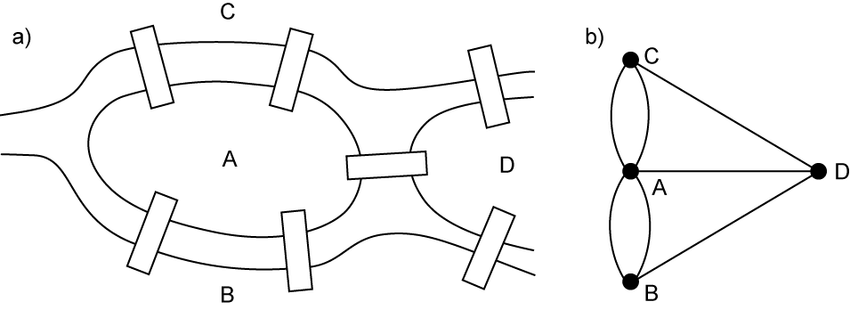
\includegraphics[scale=0.5]{figuras/Koenigsberg.png}
  \captionsetup{font=small,position=below,skip=-1pt}
   \caption*{Fonte: Boguslawski, Pawel~\cite{Koenigsberg}.}
   \label{Konigsberg}
\end{figure}

A prova de Euler mostra que quando se quer modelar algum problema não é necessário considerar todas as variáveis existentes neles, mas o essencial para a solução. Nesse caso o mais importante foi esquematizar o problema usando Grafos e, principalmente, analisar uma estrutura intrínseca ao Grafo.

Com a solução do problema surge a área da matemática chamada Grafos que é a base matemática para o que chamamos em redes. Essa nomenclatura varia de área para área; na física, por exemplo, são sinônimos enquanto na computação Grafos estão relacionados à problemas de fluxo~\cite{Grafos01,Grafos} e redes são utilizados para problemas visando a estrutura do Grafo e suas interações~\cite{network,networks}. Nesse trabalho usaremos os dois como sinônimos.

\section{Conceitos Fundamentais}

Um Grafo $G(\mathpzc{N} ,\mathpzc{L})$ é uma dupla na qual $\mathpzc{N} = \{\nu_0,\nu_1,\nu_2,...,\nu_i,...\}$ é um conjunto não vazio de elementos chamados de vértices ou 
nós e $\mathpzc{L}$ é um conjunto não vazio de pares 
de elementos de $\mathpzc{N}$ chamados de 
arestas ou ligações. Dessa forma podemos definir $N = |\mathpzc{N}|$ que mensura a quantidade de vértices que há em $G$ e $L= |\mathpzc{L}|$ que mensura o número de arestas. Essas quantidades também são chamadas de ordem e tamanho~\cite{Grafos}, respectivamente.

A partir dessa definição de redes é possível definir a Matriz de Adjacência que guarda a informação de 
conexões entre os nós. Seja uma matriz $A$ quadrada de tamanho $N \times N$, cada elemento da matriz segue a seguinte regra:
\[   
  A_{i,j} = 
     \begin{cases}
       1 \quad 
       \text{se } (\nu_i,\nu_j)\in \mathpzc{L}\\
       0 \quad \text{caso contrário.} \\
     \end{cases}
\]

A partir dela surgem características importantes de redes. Se $A_{i,j} = A_{i,j}\; \forall \nu_i,\nu_j \in \mathpzc{N}$ então a rede é chamada de não direcionada; se $\exists \nu_i\neq \nu_j$ tal que 
$A_{i,j} \neq A_{j,i}$ 
ela é chamada de direcionada. Isso pode ter diferentes interpretações a depender do contexto, por exemplo na rede de amigos do \textit{Facebook}, se o usuário A é amigo de B, então B é amigo de A. No caso do \textit{Instagram} se A segue B, não necessariamente B segue A. No primeiro caso é natural modelarmos utilizando redes não direcionadas, enquanto no segundo usamos redes direcionadas.

Uma alternativa para registrar a informação da Matriz de Adjacência é através da lista de vizinhos. Dois vértices $\nu$ e $\mu$ são vizinhos se existe uma ligação entre $\nu$ e $\mu$, assim é denotado $\eta(\nu)$ o conjunto de vizinhos do vértice $\nu$ para redes não direcionadas. Em redes direcionadas, existem dois tipos de vizinhos: os que se conectam a um nó e os que são conectados por um nó. Portanto, denotaremos $\eta_{in}(\nu)$ todos os vizinhos que têm ligação que chega em $\nu$ e $\eta_{out}(\nu)$ todos os vizinhos que têm ligação que sai de $\nu$.

Por fim, é possível adicionar propriedades às nossas ligações. As propriedades têm várias interpretações nos problemas: em uma rede de canos de esgoto, o fluxo que passa em um cano pode ser um peso e em redes de \textit{Facebook} o nível de amizade pode ser um peso das ligações entre usuários. 
Além disso, pode-se também adicionar pesos aos vértices, representando alguma característica não-topológica dos mesmos, como, exemplo, idade de um indivíduo.
Formalmente, um Grafo ponderado $G(\mathpzc{N},\mathpzc{L},\Theta,\Xi\left(\nu_i,\nu_j\right))$ é formado por um conjunto de nós $\mathpzc{N}$, um conjunto de arestas $\mathpzc{L}$ e um mapeamento $\Theta: \mathpzc{N}\mapsto \mathpzc{S}$ que representa uma rede ponderada nos nós e 
$,\Xi\left( \nu,\mu \right): \mathpzc{L}\mapsto \mathpzc{R}$ na qual $\mathpzc{R}$ e $\mathpzc{S}$ são propriedades da rede que podem ser quantitativas ou qualitativas, vetoriais ou não. Nesse caso é definido uma generalização da matriz da Matriz de Adjacência, seja 
$w_{\nu,\mu}$ o peso da ligação $(\nu,\mu$) então definimos a Matriz de Adjacência Ponderada como:
\[   
  W_{i,j} = 
     \begin{cases}
       w_{\nu_i,\nu_j} \quad 
       \text{se } (\nu_i,\nu_j)\in \mathpzc{L}\\
       0 \quad \text{caso contrário.} \\
     \end{cases}.
\]

A Figura \ref{fig:redes} mostra um exemplo 
de uma rede com 8 nós enumerados de 0 a 7, com 12 arestas e a matriz de adjacência $A_{i,j}$ .

\begin{figure}[H]
  \centering
  \captionsetup{font=normalsize,skip=0.8pt,singlelinecheck=on,labelsep=endash}
  \caption{Ilustração de Redes e seus Parâmetros}
  \begin{tikzpicture}[make origin horizontal center of bounding box]
    \draw[black, thick] (0,0) -- ($(2,0)+(0,1.5)$);
    \draw[black, thick] (0,0) -- ($(-2,0)+(0,2)$);
    \draw[black, thick] (0,0) -- ($(-2,0)+(0,-1)$);
    \draw[black, thick] (0,0) -- ($(-3.5,0)+(0,-1)$);
    \draw[black, thick] (-3.5,-1) -- ($(-4,0)+(0,1)$);
    \draw[black, thick] (-2,-1) -- ($(-4,0)+(0,1)$);
    \draw[black, thick] (-4,1) -- ($(-2,0)+(0,2)$);
    \draw[black, thick] (-2,-1) -- (-3.5,-1);
    \draw[black, thick] (-4,1) -- (-5.5,0);
    \draw[black, thick] (-3.5,-1) -- (-5.5,0);
    \draw[black, thick] (-4,1) -- (-5.5,-2.5);
    \draw[black, thick] (-3.5,-1) -- (-5.5,-2.5);

    \draw[black, fill=white] ($(0,0) + (0,0)$) circle [radius=0.3] node {0};
    \draw[black, fill=white] ($(2,0) + (0,1.5)$) circle [radius=0.3] node {1};
    \draw[black, fill=white] ($(-2,0) + (0,2)$) circle [radius=0.3] node {5};
    \draw[black, fill=white] ($(-2,0) + (0,-1)$) circle [radius=0.3] node {2};
    \draw[black, fill=white] ($(-4,0) + (0,1)$) circle [radius=0.3] node {4};
    \draw[black, fill=white] ($(-5.5,0) + (0,0)$) circle [radius=0.3] node {6};
    \draw[black, fill=white] ($(-3.5,0) + (0,-1)$) circle [radius=0.3] node {3};
    \draw[black, fill=white] ($(-5.5,0) + (0,-2.5)$) circle [radius=0.3] node {7};
    
    \node at (4,3) {$N = 8$};
    \node at (4,2.5) {$L = 12$};
    \node at (2.5,-1) {$A = $};
    \draw [decorate,
    decoration = {brace}] (3,-3.2) --  (3,1.2);
    \draw [decorate,
    decoration = {brace, mirror}] (7,-3.2) --  (7,1.2);
    \matrix at (5,-1)
  {

    \node {0}; & \node{1}; & \node {1}; & \node {1}; & \node {0}; & \node {1}; & \node {0}; & \node {0};  \\
    
    \node {1}; & \node{0}; & \node {0}; & \node {0}; & \node {0}; & \node {0}; & \node {0}; & \node {0};  \\

    \node {1}; & \node{0}; & \node {0}; & \node {1}; & \node {1}; & \node {0}; & \node {0}; & \node {0};  \\

    \node {1}; & \node{0}; & \node {1}; & \node {0}; & \node {1}; & \node {0}; & \node {1}; & \node {1};  \\

    \node {0}; & \node{0}; & \node {1}; & \node {1}; & \node {0}; & \node {1}; & \node {1}; & \node {1};  \\

    \node {1}; & \node{0}; & \node {0}; & \node {0}; & \node {1}; & \node {0}; & \node {0}; & \node {0};  \\

    \node {0}; & \node{0}; & \node {0}; & \node {1}; & \node {1}; & \node {0}; & \node {0}; & \node {0};  \\
    
    \node {0}; & \node{0}; & \node {0}; & \node {1}; & \node {1}; & \node {0}; & \node {0}; & \node {0};  \\
  };
  \end{tikzpicture}
  \captionsetup{font=small}
  \caption*{Ilustração de uma rede, das suas quantidades de ligações $L$, de nós $N$ e da Matriz de Adjacência $A$.\\ Fonte: Elaborado pelo autor}
  \label{fig:redes}
\end{figure}

\section{Métricas estruturais de Redes}

Como discutido anteriormente é muito importante estudarmos a estrutura da rede.
Para um entendimento melhor dessa estrutura existem várias métricas~\cite{Costa2007} relacionadas à topologia da rede podendo ser classificadas como globais ou locais. 
Métricas globais de redes são medidas que fornecem informações sobre as propriedades e características de uma rede como um todo, em oposição às métricas locais que se concentram em elementos individuais dentro da rede, como nós ou arestas. 
Ao final
desta seção, a Figura \ref{Exemplo01} e as Tabelas \ref{tab:Global}-\ref{tab:centralidade_rede} apresentam um exemplo com aplicações dessas métricas.

\subsection{Métricas Globais de Redes}

Seja \( G' \) um grafo \( G'(\mathpzc{N}', \mathpzc{L}') \) tal que \( \mathpzc{N}' \subseteq \mathpzc{N} \) e \( \mathpzc{L}' \subseteq \mathpzc{L} \), \( G' \) então é definido como sub-grafo de $G$, pois contém vértices e arestas que também estão em $G$ . Assim uma componente de um grafo \( G \) como um subgrafo que satisfaz duas condições: conectividade interna e maximalidade. Conectividade interna significa que, para qualquer par de vértices \( u, v \in C \), existe um caminho em \( C \) que conecta \( u \) a \( v \) usando apenas vértices e arestas de \( C \), ou seja, o subgrafo induzido por \( C \) é conexo. Maximalidade implica que não é possível adicionar nenhum outro vértice ou aresta ao subgrafo \( C \) sem perder a propriedade de conectividade interna, ou seja, \( C \) é maximal com respeito à conectividade.


Sejam dois vértices $\nu,\mu \in \mathpzc{N}$ é dito que existe um caminho entre $\nu$ e $\mu$ se existe uma sequência de vértices $\zeta_1,\zeta_{2},...,\zeta_m | (\zeta_{s},\zeta_{s+1}) \in \mathpzc{L}$, $\zeta_1=\nu$, $\zeta_m=\mu$, na qual não há repetição de vértices ou arestas. O comprimento de um caminho é dado por sua quantidade de arestas. 
Podem existir vários caminhos 
entre $\nu$ e $\mu$, portanto a distância geodésica entre dois vértices $d_{\nu,\mu}$ é definida como o menor comprimento dentre todos os caminhos entre $\nu$ e $\mu$. Mediante essa definição, é possível construir a métrica 
global $\left\langle d \right\rangle $
chamada distância geodésica média da rede:
\begin{equation}
     \left\langle d \right\rangle  = \sum_{\substack{\nu\neq\mu}} \frac{d_{\nu,\mu}}{N\cdot(N-1)}.
\end{equation}
Esse valor nos dá a informação sobre o quanto em média é necessário caminhar na rede de um nó para outro. No caso de redes ponderadas considere dois vértices $\nu,\mu \in \mathpzc{N}$ é dito que existe um caminho entre os dois nós se existe uma sequência de vértices $\zeta_1,\zeta_{2},...,\zeta_m | (\zeta_{s},\zeta_{s+1}) \in \mathpzc{L}$, $\zeta_1=\nu$, $\zeta_m=\mu$ e para esse caminho é atribuído um peso $\sum_{s}w_{\zeta_s,\zeta_{s+1}}$, portanto o menor caminho é aquele que minimiza 
$\sum_{s}w_{\zeta_s,\zeta_{s+1}}$ e seu valor será a distância geodésica $d_{\nu,\mu}^w$. Contudo a concepção de menor caminho entre dois pontos pode depender do problema, por exemplo para se achar a resistência equivalente em uma rede de resistores pode se utilizar da mínima resistência ou de máxima corrente.

Outro valor importante é o chamado diâmetro $d = \max\limits_{\nu,\mu} d_{\nu,\mu}$ que é a maior distância geodésica da rede, ele reflete o maior número de etapas necessárias para viajar entre os dois vértices mais distantes na rede, fornecendo uma medida da ``extensão'' da rede em termos da sua conectividade. 
Esse valor está relacionado a um tipo de rede chamada redes de pequeno mundo, \citeonline{Watts1998} definem que uma rede é dita de pequeno mundo quando $\left\langle d\right\rangle \propto \log(N)$, redes com essa propriedades apresentam uma pequena distância entre qualquer par de nós e facilmente a informação pode propagar na rede.

Uma outra métrica a ser avaliada é o número de conexões que cada nó contém. É definido o grau $k_{\nu}$ como o número de conexões (ou vizinhos) que o nó $\nu$ possui para redes não direcionadas. Para redes direcionadas existe uma divisão entre $k^{in}_{\nu}$ e $k^{out}_{\nu}$ para os nós que pertencem a $\eta_{in}(\nu)$ e $\eta_{out}(\nu)$, respectivamente. Pode-se achar os valores $k^{in}_{\nu_i}$ e $k^{out}_{\nu_i}$ a partir da Matriz de Adjacência da seguinte forma:
\begin{equation}
    k^{in}_{\nu_i} = \sum_{j} A_{j,i}, \qquad  k^{out}_{\nu_i} = \sum_{j} A_{i,j}.
\end{equation}
Nessa formulação é possível definir o grau em redes ponderadas  
$k^w_{\nu_i}$ substituindo $A_{i,j}$ por $W_{i,j}$. 
Além disso é possível também definir o grau médio $\left\langle k \right\rangle$ da rede
\begin{equation}
  \left\langle k \right\rangle = \sum\limits_{\nu\in\mathpzc{N}}\frac{k_{\nu}}{N} = 2\frac{L}{N}.
  \label{grau_tamanho}
\end{equation}
Esse valor tem bastante importância quantitativa quando o objetivo é trabalhar com distribuições de graus.
Analogamente, pode-se definir o grau de entrada ou de saída médio, bem como o grau ponderado médio da rede.

Outras duas métricas importantes são a densidade $\rho(G)$ e a reciprocidade $rc(G)$. A primeira mede a razão entre a quantidade de arestas dentro do grafo $G$ pela quantidade total de arestas que o grafo pode suportar. Já a segunda nos apresenta a fração de arestas que existem em ambas as direções; no caso trivial de redes não direcionadas esse valor é igual a 1.
\[   
  \rho(G) = 
     \begin{cases}
      \frac{2L}{N\cdot(N-1)} \quad \text{se a rede for não direcionada, ou }\\
      \frac{L}{N\cdot(N-1)} \quad \text{se a rede for direcionada;} \\
     \end{cases}
\]
\begin{equation}
  rc(G) = \frac{\sum\limits_{i,j} A_{i,j}A_{j,i}}{\sum\limits_{i,j } A_{i,j}}.
\end{equation}

Por fim existe uma métrica para analisar o Agrupamento de uma Rede, ou seja quanto que os vértices estão unidos. Essa métrica será definida a partir da probabilidade de um vizinho do nó $\nu_i$ estar conectado com outro vizinho de $\nu_i$
\begin{equation}
  C(G) = \frac{\sum\limits_{(i,j,k): i\neq j \neq k}A_{i,j}A_{j,k}A_{k,j}}{\sum\limits_{(i,j,k): i\neq j \neq k}A_{i,j}A_{j,k}} = 3\frac{\#\text{Triângulos}}{\#\text{Tríades}},
  \label{clustering2}
\end{equation}
em que $\#$ significa número de alguma coisa, no caso estamos contando o número de triângulos e o número de tríades que aparecem na rede. Essa é a definição do que chamamos de Agrupamento Global, podemos também definir o Agrupamento Local $C(\nu)$ e por ele o Agrupamento Médio $\langle C\rangle$:
\begin{equation}
  C(\nu) = 2\frac{\#\text{Triângulos que contém o nó }\nu}{\#\text{Tríades que contém o nó }\nu}, \qquad   \langle C \rangle = \sum\limits_{\nu \in \mathpzc{N}}\frac{C(\nu)}{N}.
  \label{clusteringlocal}
\end{equation}

A Figura~\ref{Exemplo01} ilustra uma rede e 
  suas Métricas Globais: menor caminho médio $\langle d \rangle$, diâmetro $d$, grau médio $\langle k \rangle$, densidade $\rho$, Agrupamento $C$, Agrupamento Médio $\langle C \rangle$. Os valores do \#Triângulos, \#Triades e o Agrupamento se encontram na Tabela \ref{tab:Global}.

\begin{figure}[H]
  \centering
  \captionsetup{font=normalsize,skip=0.8pt,singlelinecheck=on,labelsep=endash}
  \caption{Ilustração de Redes e suas Métricas Globais. Fonte: Elaborado pelo autor}
  \begin{tikzpicture}[make origin horizontal center of bounding box]
    \draw[black, thick] (0,0) -- ($(2,0)+(0,1.5)$);
    \draw[black, thick] (0,0) -- ($(-2,0)+(0,2)$);
    \draw[black, thick] (0,0) -- ($(-2,0)+(0,-1)$);
    \draw[black, thick] (0,0) -- ($(-3.5,0)+(0,-1)$);
    \draw[black, thick] (-3.5,-1) -- ($(-4,0)+(0,1)$);
    \draw[black, thick] (-2,-1) -- ($(-4,0)+(0,1)$);
    \draw[black, thick] (-4,1) -- ($(-2,0)+(0,2)$);
    \draw[black, thick] (-2,-1) -- (-3.5,-1);
    \draw[black, thick] (-4,1) -- (-5.5,0);
    \draw[black, thick] (-3.5,-1) -- (-5.5,0);
    \draw[black, thick] (-4,1) -- (-5.5,-2.5);
    \draw[black, thick] (-3.5,-1) -- (-5.5,-2.5);

    \draw[black, fill=white] ($(0,0) + (0,0)$) circle [radius=0.3] node {0};
    \draw[black, fill=white] ($(2,0) + (0,1.5)$) circle [radius=0.3] node {1};
    \draw[black, fill=white] ($(-2,0) + (0,2)$) circle [radius=0.3] node {5};
    \draw[black, fill=white] ($(-2,0) + (0,-1)$) circle [radius=0.3] node {2};
    \draw[black, fill=white] ($(-4,0) + (0,1)$) circle [radius=0.3] node {4};
    \draw[black, fill=white] ($(-5.5,0) + (0,0)$) circle [radius=0.3] node {6};
    \draw[black, fill=white] ($(-3.5,0) + (0,-1)$) circle [radius=0.3] node {3};
    \draw[black, fill=white] ($(-5.5,0) + (0,-2.5)$) circle [radius=0.3] node {7};
    
    \node at (4,1.25) {$\langle l \rangle = 
    1.68$};
    \node at (4,0.75) {$d = 3$};
    \node at (4,0.25) {$\langle k \rangle = 
    3$};
    \node at (4,-0.25) 
{$\rho = 12/28$};
    \node at (4,-0.75) {$C = 0.375$};
    \node at (4,-1.25) {$ \langle C \rangle 
    = 0.4417$};
  \end{tikzpicture}
  \label{Exemplo01}
\end{figure}

\begin{table}[H]
    \captionsetup{font=normalsize,skip=0.8pt,singlelinecheck=on,labelsep=endash}
\caption{Valores de \#Triângulos($\nu_i$), \#Tríades($\nu_i$)  e $C(\nu_i)$ do exemplo da Figura \ref{Exemplo01}.}

    \centering
    \begin{tabular}{|c|c|c|c|c|c|c|c|c|}%
        \hline%
         nó &0&1&2&3&4&5&6&7\\%         
        \hline%
    \#Triângulos($\nu_i$)&1&0&2&4&3&0&1&1\\%
        \hline%
        \#Tríades($\nu_i$)&6&0&3&10&10&1&1&1\\%%\#Triades(\nu_i)&6&0&3&10&0&10&1&1\\%
        \hline%
        \#C($\nu_i$)&0.167&0.000&0.667&0.400&0.300&0.000&1.000&1.000\\%
        \hline%
    \end{tabular}%
    \label{tab:Global}
\end{table}



\subsection{Métricas Locais de Centralidade}


Ao estudar redes o interesse está voltado em entender suas estruturas e propriedades, isso já é possível dadas as métricas que apresentamos anteriormente. É importante destacar que essas métricas globais oferecem uma análise abrangente da topologia da rede, revelando suas propriedades e comportamentos coletivos que podem estar diluídas na rede ou concentradas em nós específicos. Portanto estudar os nós em si e a sua importância perante a rede é necessário; para isso são usadas as chamadas Métricas Locais de Centralidade. 

Quando falamos de Métricas de Centralidade o interesse é estudar a importância topológica de cada nó perante a rede. 
Mas em que sentido seria essa importância? Depende do problema, talvez seja necessário estudar qual o autor mais importante em uma rede de citações de artigos~\cite{Leydesdorff2011} ou qual indivíduo devemos retirar de uma rede criminosa para desfazer a rede~\cite{deAndrade2021}. Para ambos os casos e vários outros exemplos existem métricas apropriadas para atingir tais objetivos.

A métrica inicial a ser analisada consiste na contagem das conexões individuais de cada nó, representada pelo grau $k_\nu$. Ao conduzir essa avaliação, identificamos o nó central como aquele que apresenta o grau $k_\nu$ mais elevado, objetivando, assim, encontrar o nó com a maior quantidade de conexões que é a Centralidade de Grau (\gls{CG}).

A segunda métrica importante é a Centralidade de Excentricidade (\gls{CE}). Essencialmente, a CE de um nó é determinada calculando-se o recíproco da maior distância que separa esse nó de qualquer outro nó na rede. Ela exibe a distância máxima que um nó precisa percorrer para alcançar o ponto mais remoto da rede. O nó cuja maior distância é a menor entre todos os nós da rede é então identificado como o mais central. Formalmente $CE(\nu)\; \forall \nu \in \mathpzc{N}$ é definida como:
\begin{equation}
  CE(\nu) = \frac{1}{\max\limits_{\mu} d_{\nu,\mu}}.
\end{equation}
Nessa mesma ideia é propício avaliar outras duas métricas parecidas: Centralidade de Proximidade (\gls{CP}) e Centralidade Harmônica (\gls{CH}). Em ambas o interesse é entender qual é o nó mais central a partir de quanto ele dista dos outros, a diferença entre as duas é que a primeira é calculada pelo inverso da média aritmética e a segunda com a média harmônica:
\begin{equation}
  \gls{CP}(\nu) = \frac{N - 1}{\sum\limits_{\mu \neq \nu} d_{\nu,\mu}},
\end{equation}
\begin{equation}
  \gls{CH}(\nu) = \frac{1}{N - 1}\sum_{\mu \neq \nu}\frac{1}{d_{\nu,\mu}}.
\end{equation}

Uma generalização da \gls{CP} e \gls{CE} é a Centralidade de
Média-$p$ ($C_p$)~\cite{Andrade2019}. A ideia desta medida de centralidade é usar a noção de média
generalizada das distâncias. Ela é definida como:
\begin{equation}
  C_p(\nu) = 
  \begin{cases}
    \left(\frac{\sum\limits_{\mu \neq \nu } d_{\nu,\mu}^p}{N - 1}\right)^{-\frac{1}{p}} &\text{se $p \neq 0$},\\
    \left(\prod\limits_{\mu \neq \nu} d_{\nu,\mu}\right)^{-\frac{1}{N - 1}} &\text{se }p = 0.
  \end{cases}
\end{equation}

Entretanto a importância de um nó não está associada somente a sua distância 

com os outros nós da rede, existem aqueles que são importantes por 

intermediarem
conexões entre nós. Por exemplo,
considere a rede mundial
de 
aeroportos, que seja construída a partir de nós como sendo os aeroportos e as ligações sendo as viagens entre aeroportos. Nessa situação, imagine que tenha um país altamente conectado entre si, contudo ele só tem um aeroporto que liga esse país ao exterior, esse nó é importante não pela distância dele para os outros aeroportos mas porque ele é o principal e 
a única conexão
entre o exterior e o país.

Para ser possível detectar e mensurar esse tipo de importância, considere
$\mathbb{L}_{\mu,\zeta}$ o número de caminhos mínimos que vão de $\nu$ para $\mu$ e 
$\mathbb{L}^{\nu}_{\mu,\zeta}$ 
o número de mínimos caminhos entre $\mu$ e $\zeta$ e passam pelo vértice
$\nu$. Portanto, podemos definir a Centralidade de Intermediação (\gls{CB}) como
\begin{equation}
  \gls{CB}(\nu) = \frac{1}{(N - 1)(N - 2)} \sum\limits_{\mu \neq \zeta} \frac{\mathbb{L}^{\nu}_{\mu,\zeta}}{\mathbb{L}_{\mu,\zeta}},
\end{equation}
em que $\mu$ e $\zeta$ são diferentes do nó $\nu$.

Quando se trata de analisar uma rede empresarial, é fundamental reconhecer a relevância do CEO para a organização. No entanto, é importante notar que o CEO mantém comunicação direta apenas com os líderes de cada região da empresa, enquanto esses líderes não necessariamente se comunicam diretamente entre si. Portanto, onde reside a indicação da importância do CEO? A resposta a essa indagação repousa no fato de que o CEO estabelece conexões com indivíduos influentes na rede, um aspecto que não é capturado pelas métricas 
mencionadas até então
de análise de rede. Definimos a Centralidade de Autovetor (\gls{CA}) como:
\begin{equation},
  \gls{CA}(\nu_i) = \frac{1}{\lambda}\sum_{\nu_j}A_{i,j}\; \gls{CA}(\nu_j),
\end{equation}
na qual $\lambda$ é o maior autovalor associado à matriz de adjacência de rede. A importância dessa conexão é que os autovetores e autovalores capturam informações sobre como a informação flui na rede. Se um nó estiver conectado a outros nós importantes (ou seja, nós com alta centralidade), ele terá uma alta centralidade de autovetor, mesmo que tenha poucas conexões diretas. Em contrapartida, se um nó estiver conectado principalmente a nós periféricos, terá uma baixa centralidade de autovetor.

Com o advento das páginas da \textit{internet} é preciso metrificar quais são os \textit{sites} mais importantes. Para isso seria importante não só levar em consideração quem está em posição privilegiada, mas também como essa posição é mitigada pelo número de ligações, portanto~\cite{page1999pagerank} publicaram uma nova métrica que consegue quantificar isso chamada de \textit{PageRank}. Essa métrica é utilizada pelo \textit{Google} para analisar a importância de \textit{sites} na \textit{internet}. Considere um usuário que navega pela \textit{internet} e está em um \textit{site} $\nu_j$ e deseja ir para outro. Existe uma probabilidade $\alpha$ de o usuário seguir um \textit{link} dentro do \textit{site} atual e ir para outro que ele aponta, e uma probabilidade $1 - \alpha$ de ele não seguir essa estrutura e ir para um \textit{site} aleatório. Eles definiram o \textit{PageRank} do nó $\nu_j$ como:
\begin{equation}
  \gls{PR}(\nu_j) =1 - \alpha + \alpha\times \sum_{j \neq i} A_{i,j}\frac{\gls{PR}(\nu_i)}{k^{out}_{\nu_j}}.
\end{equation}

\citeonline{Carmi2007} formularam o algoritmo \textit{K-Shell} que se concentra em decompor a rede não direcionada em camadas, onde cada camada representa um subconjunto de nós com uma centralidade mínima, conhecida como o ``grau mínimo'' K. Inicialmente, os nós são ordenados por grau em ordem decrescente, e aqueles com menor grau são iterativamente removidos até que nenhum nó com grau menor ou igual a K permaneça na rede. Esse processo gera uma sequência de camadas (\textit{K-Shells}), onde as camadas mais internas contêm nós de alta centralidade, enquanto as camadas mais externas contêm nós de menor centralidade. 
O seguinte algoritmo realiza a descomposição em \textit{K-Shells}: 
\begin{enumerate}
    \item É inicializado \( k = 1 \). Este é o nível inicial de k-shell.
    \item Encontre e remova todos os vértices de grau \( k \). Atribua a esses vértices o k-shell \( k \).
    \item Após a remoção, reduza em 1 o grau de todos os vértices adjacentes aos removidos.
    \item Se ainda existirem vértices de grau \( k \) no grafo residual, repita o passo 2 e 3 para esses vértices.
    \item Incremente \( k \) para \( k + 1 \) e verifique se existem vértices de grau \( k \) no grafo residual. Se sim, repita os passos 2 a 4.
    \item Continue o processo até que não reste nenhum vértice no grafo.
    \item O algoritmo termina quando todos os vértices são atribuídos a um k-shell e o grafo está completamente decomposto.
\end{enumerate}

A tabela \ref{tab:centralidade_rede} apresentada resume os valores de diferentes métricas de centralidade para uma rede específica, conforme ilustrado na Figura \ref{fig:redes}. Cada coluna representa um nó individual da rede, numerados de 0 a 7, e cada linha descreve uma métrica específica de centralidade: Centralidade de Excentricidade (\gls{CE}), Centralidade de Grau (\gls{CG}), K-shell (\gls{CK}), Centralidade de Proximidade (\gls{CP}), Centralidade de Harmonia (\gls{CH}), Centralidade de Betweenness (\gls{CB}) e Centralidade de Autovalor (\gls{CA}). Observa-se uma variabilidade entre os nós nas medidas de Centralidade de Excentricidade (\gls{CE}), com nós como o 1, 5, 6 e 7 exibindo valores inferiores, indicando uma posição mais periférica na rede. O nó 3 destaca-se com valores altos tanto na Centralidade de Grau (\gls{CG}) quanto na Centralidade de Betweenness (\gls{CB}), sublinhando sua influência central como ponto de conexão e intermediário crucial nas interações da rede.
\begin{table}[H]
    \captionsetup{width=13.5cm}
    \caption{Valores de diferentes métricas de centralidade do exemplo da Figura \ref{Exemplo01}.}
    \centering
    \begin{tabular}{crrrrrrrr}
        \toprule
        & nó 0 & nó 1 & nó 2 & nó 3 & nó 4 & nó 5 & nó 6 & nó 7 \\
        \midrule
        \midrule
        \gls{CE} & 0.5 & 0.333 & 0.5 & 0.5 & 0.5 & 0.333 & 0.333 & 0.333 \\
        \gls{CG} & 0.571 & 0.143 & 0.429 & 0.714 & 0.286 & 0.714 & 0.286 & 0.286 \\
        \gls{CK} & 2 & 1 & 2 & 2 & 2 & 2 & 2 & 2 \\
        \gls{CP} & 0.7 & 0.438 & 0.636 & 0.778 & 0.583 & 0.7 & 0.538 & 0.538 \\
        \gls{CH} & 5.5 & 3.5 & 5.0 & 6.0 & 5.833 & 4.5 & 4.333 & 4.333 \\
        \gls{CB} & 0.333 & 0.0 & 0.032 & 0.294 & 0.032 & 0.214 & 0.0 & 0.0 \\
        \gls{CA} & 0.353 & 0.101 & 0.385 & 0.511 & 0.239 & 0.486 & 0.285 & 0.285 \\
        \bottomrule
    \end{tabular}
    \caption*{Valores de diferentes métricas de centralidade calculados para a rede ilustrada na Figura \ref{fig:redes}, os valores foram calculados utilizando a biblioteca Networkx.\\ Fonte:~\cite{hagberg2008exploring}.}
    \label{tab:centralidade_rede}
\end{table}

\subsection{Métricas em Redes Ponderadas}

Na seção anterior, foram discutidas diversas métricas tradicionais empregadas na análise de redes e grafos. Embora essas métricas sejam fundamentais e amplamente reconhecidas no campo da análise de redes, é importante reconhecer que elas apresentam limitações. As suas principais dificuldades estão em ao considerar ponderação nas arestas metrificar somente com viés de estrutura da rede e pouco se leva em conta uma real mistura entre esses dois valores. 

\citeonline{Rgo2019} criaram uma métrica para estudar co-autoria em artigos acadêmicos levando em conta a força entre as ligações dos vizinhos de cada autor e também como essa ligação é importante perante outras ligações entre vizinhos. A 
métrica de Utilidade é definida como:
\begin{equation}
  \gls{UT}(\nu) = \sum_{\substack{\mu \in \eta(\nu)}} \left(\frac{w_{\nu,\mu}}{k^w_\nu}+ \frac{w_{\nu,\mu}}{k^w_\mu} + \frac{w_{\nu,\mu}^2}{k^w_\nu k^w_\mu}\right)
\end{equation}
O primeiro termo quantifica o quão importante é a ligação entre o sítio $\nu$ com $\mu$ em relação às ligações de $\nu$, já o segundo é em relação às ligações de $\mu$ e o terceiro termo é um termo misto. Para redes sem ponderação $w_{\nu,\mu} = 1$, $k_\nu^w = k_\nu$~\cite{Jackson1996}.
\cite{Qi2012} apresentam a chamada Centralidade Laplaciana (\gls{CL}) na qual tentam mensurar a importância de um nó pela falta que ele faz se o retirarmos da rede (essa premissa vai ser muito presente na literatura atual). Porém como os autores mostram essa métrica não é totalmente local, carregando informação de vizinhos de vizinhos, contudo ela não é definida bem em redes direcionadas.
Seja $W$ a Matriz de Adjacência ponderada e seja a matriz $X$ uma matriz diagonal com cada elemento $X_{i,i} = \sum_{j \in \eta(\nu_i)}w_{\nu_i,\nu_j}$, pode se definir uma matriz chamada de Laplaciana~\cite{networks} $L^a$ como $L^a_{i,j} = X_{i,j} - W_{i,j}$. Sejam
${\lambda_{i}}$ os auto-valores de $L^a$. É possível definir a Energia do grafo $G$ como:
\begin{equation}
    E(G) = \sum_{i} \lambda_{i}^2 = \sum_{i}X_{i,i}^2 + 2\times\sum_{i < j}w_{\nu_i,\nu_j}^2,
\end{equation}
Seja $G_\nu$ o grafo $G$ com a ausência do nó $\nu$, assim é possível definir a \gls{CL} como:
\begin{equation}
  \gls{CL}(\nu) = \frac{E(G_\nu) - E(G)}{E(G)}.
\end{equation}

Por fim
\citeonline{deAndrade2021} estabelecem uma centralidade baseada na lei da gravitação universal de Newton, chamada de Centralidade Gravitacional (\gls{CGR}), ela leva em consideração as distâncias entre os nós e a ponderação nos nós da rede. A intuição dessa métrica está atrelada ao fato de que pessoas com características relevantes como conhecimento, idade, etnias,posição social, dentre outras os tornam mais ou menos influentes e atrativos na sua rede de contatos. Assim \gls{CGR}($\nu$) é calculada como:

\begin{equation}
  \gls{CGR}(\nu) =\sum_{\mu \neq \nu}\frac{w_\nu w_\mu}{(d_{\nu,\mu}^w)^{1/s}}.
\end{equation}
Na qual $w_\nu$ é o peso do nó $\nu$ e $s$ um parâmetro de controle que para a lei da gravitação $s = \frac{1}{2}$.

\section{Modelos de Formação de Redes}

Na seção anterior, foram abordadas as métricas utilizadas para quantificar a estrutura de redes. Então, dado um grafo $G$ é possível extrair suas propriedades. Contudo, surge a questão de saber se é possível criar uma rede que contenha determinadas propriedades quando essas são fornecidas. Portanto, nesta seção, serão discutidos os principais modelos empregados na formação de redes artificiais. Dois modelos de formação de redes amplamente utilizados na teoria das redes complexas são a Rede de Erdös-Rényi (ER) e o Modelo de Configuração. A Rede de Erdös-Rényi é uma abordagem clássica que gera redes aleatórias, onde a probabilidade de existência de uma aresta entre dois nós é independente e pré-definida. Por outro lado, o Modelo de Configuração permite criar redes com nós possuindo graus específicos, sendo útil para estudar como diferentes distribuições de grau afetam as propriedades da rede, como redes de escala-livre, e para a geração de redes sintéticas com características semelhantes às redes reais, o que é valioso em estudos empíricos e modelagem de sistemas complexos. Ambos os modelos desempenham papéis fundamentais na análise e modelagem de redes complexas em diversos domínios.

\subsection{Rede de Erdös-Rényi}

Um dos primeiros modelos que conseguiu ter sucesso na geração sintética de redes foi o de Erdös-Rényi que iniciou os estudos de grafos (ou redes) aleatórias~\cite{Erdos:1959:pmd}. O modelo é considerado estocástico com tempo discreto partindo do pressuposto que as conexões entre os nós é algo aleatório e conseguimos retirar propriedades importantes da rede. 
Apesar de ser um modelo simples e do fato de que 
poucas de suas 
propriedades aparecem em redes reais, é interessante estudar esse modelo por motivos históricos e também podemos aprender muito com ele.

Seja $G(\mathpzc{N},p)$ um grafo não direcionado que segue o modelo de Erdös-Rényi. Nesse modelo temos fixados o conjunto de vértices $\mathpzc{N}$ e temos uma probabilidade $p$ para que cada ligação 
possível seja criada. Podemos construir a rede da seguinte forma:
\begin{enumerate}
  \item Crie $N$ vértices;
  \item Selecione um vértice $\nu$ e outro vértice $\mu$ e tente os conectar com probabilidade $p$, caso consiga a ligação é criada, caso contrário salvamos que ela não existe;
  \item Fazemos 2 até testarmos todas as possíveis ligações.
\end{enumerate}

Dada a descrição que acabamos de dar do modelo podemos estudar como suas métricas se comportam. O primeiro parâmetro a ser estudado é o grau. Dado um nó qualquer da rede,
vamos calcular a probabilidade de ele possuir grau $k$. Observe que a partir de um determinado nó, existem $N-1$ possíveis ligações e como cada ligação é formada de forma independente com probabilidade $p$,
a probabilidade $P(k)$ de que um nó qualquer tenha grau $k$ é:
\begin{equation}
  P(k) = \binom{N - 1}{k} p^k(1-p)^{N - 1 - k},
\end{equation}
A partir da distribuição de graus conseguimos calcular facilmente o grau médio da rede, pois é uma distribuição binomial:
\begin{equation}
  \langle k \rangle = \sum_{k = 1}^{N - 1}P(k)k = \sum_{k = 1}^{N - 1}k \binom{N - 1}{k}p^k(1-p)^{N - 1 - k} = (N - 1)p.
\end{equation}
No caso em que $N$ é grande e $p$ é pequeno, é obtido o resultado que a distribuição tende a uma de Poisson 
com parâmetro $\langle k \rangle$. 
Isso deve ser analisado pois em redes reais $N$ tem essa característica, por isso esse modelo também é chamado de Rede Binomial ou Rede de Poisson. 

Outra métrica a ser avaliada é o agrupamento $C$ da rede. Podemos ver pela definição que demos na seção anterior que o agrupamento é a probabilidade de dois nós estarem ligados dado que estão ligados ao mesmo nó. 
No caso da rede Binomial, como a probabilidade das arestas são independentes,
isso é 
igual 
a probabilidade $p$:
\begin{equation}
  C(G) = p = \frac{\langle k \rangle}{N - 1}.
\end{equation}

\subsection{Modelo de Configuração}

Diferentemente do Modelo de Erdös-Rényi, no Modelo de Configuração (MC) \cite{networks}, seja um grafo com uma quantidade conhecida de $N$ nós e também informações sobre o grau de cada nó, representado por
$k_\nu$. O MC 
possui uma restrição de que a soma de todos os graus deve ser um número par, condição 
que é decorrência da relação observada na
Equação~\ref{grau_tamanho}. O modelo, Algoritmo \ref{alg:MC}, é aplicado da seguinte maneira:
\begin{enumerate}
  \item Criam-se os $N$ vértices da rede;
  \item Cada vértice $\nu$ recebe
  $\kappa_\nu = k_\nu$ ligações a serem criadas;
  \item Os vértices são ordenados de forma decrescente de grau da sequência $\{\kappa_i\}$ para facilitar a convergência do modelo;
  \item Para cada nó $\nu_i$, é realizado um processo aleatório de seleção de outro nó $\nu_j$ na rede, desde que $\nu_j$ ainda possua capacidade para formar novas ligações, denotada por 
  $\kappa_j$. Nesse cenário, estabelecemos uma conexão entre os nós $\nu_i$ e $\nu_j$, reduzindo em 1 unidade os valores de
  $\kappa_i$ e $\kappa_j$.
  \item É repetido 3 e 4 até que todas as ligações na rede sejam colocadas. 
\end{enumerate}
\begin{algorithm}[htbp]
   \caption{Modelo de Configuração}
   \label{alg:MC}
   
   \For{$\nu\in\mathpzc{N}$}{
      $\kappa_\nu \gets k_\nu$;
   }
   $\mathpzc{L} \gets \emptyset$\\
   $\text{ordem} \gets $ordenar(\{$\nu$\},\{$k_\nu$\}) \tcp{Ordena os nós por número de meias arestas, em ordem decrescente.}
   \For{$\nu \in \mathrm{ordem}$}{
     \While{$\kappa_\nu$ > 0}{
        $\mu \gets   \mathpzc{N}\setminus \{\nu\}$ \tcp{Escolhido ao acaso}
        \If{$\left[(\nu,\mu) \not\in \mathpzc{L}\right]$ $\mathbf{and }$ $\left[\kappa_\mu \neq 0\right]$}{
            $\mathpzc{L} \gets \mathpzc{L}\cup\{(\nu,\mu)\}$;\\
            $\kappa_\nu \gets \kappa_\nu - 1$;\\
            $\kappa_\mu \gets \kappa_\mu - 1$;\\
        }
    }
        
   }
   
\end{algorithm}

\begin{figure}[H]
  \centering
  \captionsetup{font=normalsize,skip=0.8pt,singlelinecheck=on,labelsep=endash}
  \caption{Ilustração do Modelo de Configuração}
  \begin{tikzpicture}
    \draw[black, thick, dotted] (0,0) -- (-1,-1);
    \draw[black, thick] (0,0) -- (1,1);
    \draw[black, thick, dotted] (0,0) -- (1,-1);
    \draw[black, thick, dotted] (0,0) -- (-1,1);
    \draw[black, fill=white] (0,0) circle [radius=0.25] node {$i$};
    \draw[black, thick, dotted] (1,1) -- (2,2);
    \draw[black, thick] (3,3) -- (2,2);
    \draw[black, thick, dotted] (3,3) -- (4,2);
    \draw[black, thick, dotted] (3,3) -- (2,4);
    \draw[black, fill=white] (3,3) circle [radius=0.25] node {$j$};
  
    \draw[black, thick, dotted] (0,3) -- (0,2);
    \draw[black, thick, dotted] (0,3) -- (0,4);
    \draw[black, thick, dotted] (0,3) -- (-1,3);
    \draw[black, thick, dotted] (0,3) -- (1,3);
    \draw[black, fill=white] (0,3) circle [radius=0.25] node {9};
  
    \draw[black, thick, dotted] (3,0) -- (4,-1);
    \draw[black, thick, dotted] (3,0) -- (2,-1);
    \draw[black, fill=white] (3,0) circle [radius=0.25] node {3};
    
    %\filldraw (0,0) circle (7pt) node[anchor=west, inner sep=0pt]{i};
  \end{tikzpicture}
  \captionsetup{font=small}
  \caption*{Funcionamento do Modelo de Configuração, escolhemos dois nós $i$ e $j$ aleatoriamente e os conectamos. Fonte: Elaborado pelo autor}
  \label{img:MC}
\end{figure}

\section{Modelos de Infecção ou Difusão}

Propagação de doenças \cite{deArruda2018,Wang2019,Bogu2002,7393962}, vírus de internet~\cite{Zhang2016,Gan2014,Yang2013}, rumores~\cite{rumor,Moreno2004,Yang2010} são alguns dos temas muito pesquisados no estudo de redes. Entender qual o principal motivo de algo se espalhar em nossa sociedade seja por quais as pessoas que difundem ou pela forma que a rede é construída é essencial para entender a difusão. Além disso, usar de modelagem matemática é essencial para boa parte desses problemas, pois apesar de termos dados sobre propagação de rumores muitas vezes não é possível coletar dados a partir da experimentação, ou seja, não podemos fazer um experimento devido a problemas logísticos ou até morais principalmente no contexto de saúde pública. Em vista disso, nesta seção serão discutidos sobre os modelos de infecção clássicos da literatura, que apesar de simples são uma boa aproximação para a epidemiologia matemática.

Na literatura existe a abordagem utilizando as equações diferenciais, no entanto em modelos tradicionais são assumidos uma mistura homogênea, o que significa que um indivíduo infectado pode infectar qualquer outro indivíduo, outrossim esse tipo de modelagem, mesmo não considerando homogeneidade, é determinística. Para prever com precisão a dinâmica de uma epidemia, é necessário de considerar o papel preciso de cada indivíduo e como as suas relações contribuem para a proliferação como um todo. É nesse sentido que é proposto um modelo com uma abordagem utilizando redes complexas, pois assim haverá o entendimento de como acontece o espalhamento de uma doença e quais os principais agentes.

Na modelagem, cada indivíduo pode se encontrar em um estado ou compartimento da infecção, esses estados podem 
refletir 
diferentes níveis de exposição ao agente patogênico, status de vacinação, ou qualquer outro fator que influencie a transmissão da doença. A interação entre os compartimentos é modelada através de equações diferenciais ou em redes. No que tange redes, para passar de um estado para outro existem taxas que podem ser de tempo contínuo ou discreto. Em caso de tempo discreto, após o incremento de um 
período (por exemplo, um dia) 
cada nó tem uma chance aleatória de alterar seu estágio com uma probabilidade que considera a taxa e, se necessário, os vizinhos dele. Enquanto no tempo contínuo, cada intervalo de tempo subsequente segue uma distribuição exponencial da soma de todas as taxas da rede, resultando na atualização de um único nó escolhido de forma aleatória 
proporcionalmente
a sua respectiva taxa para o compartimento subsequente~\cite{Gillespie1976}.

\subsection{Modelo SI}

O modelo SI descreve a propagação de uma doença em uma população, onde os indivíduos podem estar suscetíveis ou infectados, mas não se recuperam ou adquirem imunidade. A Figura~\ref{img:SI} ilustra um esquema em diagrama de blocos, mostrando a única transição possível neste modelo. 

\begin{figure}[ht]
  \centering
  \captionsetup{font=normalsize,skip=0.8pt,singlelinecheck=on,labelsep=endash}
  \caption{Esquematização do Modelo Suscetível-Infectado de contágio.}
  \begin{tikzpicture}

    \draw[->] (2,2.5) -- node[above] {$\overline{\beta}$} (3.9,2.5) ;
    
    \draw[rounded corners,drop shadow, fill=ninfect,draw=border, ultra thick] (0,2) rectangle (2,3)node[pos=.5,text= white,font=\fontsize{20}{20}\selectfont]  {$S$};
    
    \draw[rounded corners,drop shadow, fill=infect,draw=border, ultra thick](4, 2) rectangle (6,3) node[pos=.5,text= white,font=\fontsize{20}
    {20}\selectfont]  {$I$};
  \end{tikzpicture}
  \label{img:SI}
\end{figure}

descreve como a quantidade de indivíduos infectados muda ao longo do tempo. Essencialmente, ela afirma que a taxa de novos casos é proporcional ao produto do número de suscetíveis e infectados, normalizado pelo tamanho da população, e ajustado pela taxa de contato \(\beta\).

O modelo SI é um dos modelos mais simples de propagação de doenças, útil para entender a dinâmica básica de infecção. Ele assume uma população homogênea onde todos os indivíduos têm a mesma probabilidade de entrar em contato uns com os outros. Em cenários mais complexos, modelos mais sofisticados (como SIR ou SEIR) podem ser necessários para capturar características adicionais da propagação da doença, como recuperação ou períodos de incubação. Essa abordagem oferece uma base sólida para a compreensão inicial da dinâmica das doenças infecciosas e serve como um ponto de partida para modelos mais elaborados que incorporam mais detalhes sobre a transmissão e a progressão das doenças.

No modelo SI, a população é dividida em dois compartimentos: \(S(t)\), que representa a fração de indivíduos suscetíveis (aqueles que podem ser infectados) no tempo \(t\), e \(I(t)\), que representa o número de indivíduos infectados no mesmo instante. A transmissão da doença ocorre quando indivíduos suscetíveis entram em contato com indivíduos infectados e a taxa de transmissão por indivíduo é \(\beta\). Isto significa que, em média, cada indivíduo tem \(\overline{\beta}\) contatos com outros indivíduos por unidade de tempo. A taxa de novas infecções depende diretamente da probabilidade de um encontro entre um suscetível e um infectado.

Dessa forma, a taxa média de novos casos de infecção por unidade de tempo é dada por \(\overline{\beta} SI\). Isto porque cada infectado tem \(\overline{\beta}\) contatos por unidade de tempo e a fração desses contatos que são com indivíduos suscetíveis é \(S(t)\). Para modelar a dinâmica da infecção, precisamos de uma equação diferencial que descreva a taxa de variação de \(I(t)\). A equação diferencial resultante é:

\begin{align}
  \frac{dS}{dt} &= -\overline{\beta} \cdot S(t)I(t),\\
  \frac{dI}{dt} &= +\overline{\beta}\cdot S(t)I(t).
  \label{eq:SI2}
\end{align}


Esse é o modelo mais simples no estudo de infecções na qual um indivíduo só pode estar em dois estágios: suscetível ou infectado. Ao somarmos as duas equações temos:
\begin{equation}
  \frac{dS}{dt} + \frac{dI}{dt} = 0
  \rightarrow S + I = 1.
  \label{eq:SI3}
\end{equation}
Essa equação é presente em qualquer outro modelo infecção, é a equação de conservação, isto é, todos os indivíduos têm que estar em algum estágio. Substituindo (\ref{eq:SI3}) em (\ref{eq:SI2}) temos:
\begin{align}
  \frac{dI}{dt} &=\overline{\beta}(1 - I(t))I(t)\\
  \frac{1}{I(t)(1 - I(t))}\frac{dI}{dt} &= \overline{\beta}
\end{align}
Essa equação é resolvida a partir de integração dos dois lados obtendo:
\begin{equation}
  \ln{\left(\frac{I(t)}{1 - I(t)}\right)} - \ln{\left(\frac{I(0)}{1 - I(0)}\right)}  = -t\overline{\beta} \rightarrow I(t) = \frac{I(0)e^{\overline{\beta} t}}{1 - I(0) + I(0)e^{\overline{\beta} t}}
\end{equation}
Essa é a chamada equação logística que descreve o crescimento do número de infectados em função do tempo nesse modelo. Quando $t \rightarrow 0$ encontramos o valor inicial de infectados $I(0)$ e, quando $t \rightarrow \infty$, $I(t)$ converge para 1 pois com o passar do tempo todos os nós se tornarão infectados como é mostrado na Figura \ref{SI}.

\begin{figure}[H]
  \centering
  \captionsetup{font=normalsize,skip=1pt,singlelinecheck=on,labelsep=endash}
  \caption{Modelo SI}
  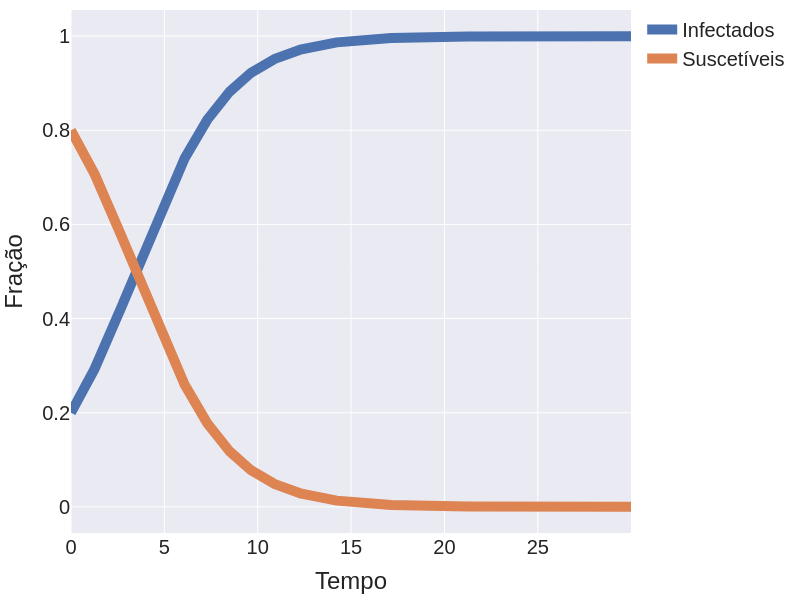
\includegraphics[scale=0.5]{figuras/SI.png}
  \captionsetup{font=small,position=below,skip=-1pt}
   \caption*{Gráfico que apresenta a evolução da infecção de um modelo SI com $I(0) = 0.2$ e $\overline{\beta} = 0.4$. Ele ilustra o crescimento de infectados ao longo do tempo em um modelo SI. Indica que, no início, há uma fração de infectados, e com o tempo, todos os indivíduos se tornarão infectados.\\Fonte: Autor.}
   \label{SI}
\end{figure}

Este modelo simplificado proporciona uma visão introdutória das dinâmicas de crescimento exponencial das infecções, ele se comporta bem 
para a modelagem de HIV~\cite{modelos} pois ou o indivíduo ao contrair a doença se torna imune ou porque após infectado jamais retorna para o compartimento de suscetível. Apesar disso ainda existem várias outras doenças que não são modeladas dessa maneira.

\subsection{Modelo SIS}

\begin{figure}[ht]
  \centering
  
  \captionsetup{font=normalsize,skip=0.8pt,singlelinecheck=on,labelsep=endash}
  \caption{Esquematização do Modelo Susceptível-Infectado-Susceptível de contágio.} 
  \begin{tikzpicture}

    \draw[->] (2,2.7) -- node[above] {$\overline{\beta}$} (3.9,2.7) ;
    \draw[->] (4.1,2.4) -- node[below] {$\overline{\gamma}$} (2.1,2.4) ;
    
    \draw[rounded corners,drop shadow, fill=ninfect,draw=border, ultra thick] (0,2) rectangle (2,3)node[pos=.5,text= white,font=\fontsize{20}{20}\selectfont]  {$S$};
    
    \draw[rounded corners,drop shadow, fill=infect,draw=border, ultra thick](4, 2) rectangle (6,3) node[pos=.5,text= white,font=\fontsize{20}
    {20}\selectfont]  {$I$};
  \end{tikzpicture}
  \label{img:SIS_}
\end{figure}

O modelo SIS, esquematizado na Figura \ref{img:SIS_},  é o modelo matemático 
que descreve a dinâmica de uma população dividida em dois compartimentos suscetíveis (S) e infectados (I) na qual é possível um indivíduo passar de infectado e voltar a ser suscetível, criando um ciclo contínuo de infecção e recuperação na população. São exemplos de doenças que podem ser modeladas a meningite, doenças venéreas e tuberculose~\cite{modelos}. O modelo segue com uma lógica idêntica ao SI adicionando um termo $\overline{\gamma}$ que representa a taxa de recuperação do indivíduo, obtendo o seguinte conjunto de equações:
\begin{align}
\frac{dS}{dt} &= -\overline{\beta} \cdot S \cdot I+ \overline{\gamma} \cdot I, \label{SIS-1} \\
\frac{dI}{dt} &= +\overline{\beta} \cdot S \cdot I- \overline{\gamma} \cdot I.\label{SIS-2} 
\end{align}
A partir desse conjunto de equações ainda é possível encontrar uma solução analítica,
obtendo as seguintes 
expressões 
para $S$ e $I$:
\begin{align}
I(t) &= \left(1 - \frac{\overline{\gamma}}{\overline{\beta}}\right)\frac{Ce^{(\overline{\beta} - \overline{\gamma})t}}{1 + Ce^{(\overline{\beta} - \overline{\gamma})t}}, \\
S(t) &= 1 - I(t).
\label{SIS_resolvido}
\end{align}
com 
$C = I(0)/(1 - I(0) - \overline{\gamma}/\overline{\beta})$. Assim a Equação \ref{SIS_resolvido} têm três tipos de comportamento dependendo de $\overline{\beta}$ e de $\overline{\gamma}$. Se $\overline{\beta} = \overline{\gamma}$ significa que a taxa de indivíduos que se tornam infectados é equivalente à taxa de recuperação que faz com que os infectados voltem a ser suscetíveis. Transforma as duas equações em $I = \frac{I(0)}{I(0)+ \overline{\beta} t}$ e $S(t) = \frac{\overline{\beta} t}{1 - S(0) + \overline{\beta} t}$ que mostra que a fração de infectados decai com $1/t$ e quando tempo tende a infinito o número de infectados tende para zero enquanto os suscetíveis converge para o tamanho da amostra. 
Se $\overline{\beta} > \overline{\gamma}$, significa que a taxa de infecção é maior que a de recuperação, e para $t \rightarrow \infty$ converge para um equilíbrio estável na qual $I(\infty) = 1 - \frac{\overline{\gamma}}{\overline{\beta}}$ e $S(\infty) = \frac{\overline{\gamma}}{\overline{\beta}}$, ou seja mesmo no infinto  ainda existirá a doença no modelo
(veja Fig. \ref{SIS}). 
Se $\overline{\beta} < \overline{\gamma}$, ou seja, a taxa de recuperação é maior que a taxa de infecção, e para $t \rightarrow \infty$ o número de infectados tende a 0 e o de suscetíveis tende a 1, ou seja, livre da doença 
(veja Fig. \ref{SIS_2}).

\begin{figure}[H]
  \centering
  \captionsetup{font=normalsize,skip=1pt,singlelinecheck=on,labelsep=endash}
  \caption{Modelo SIS}
  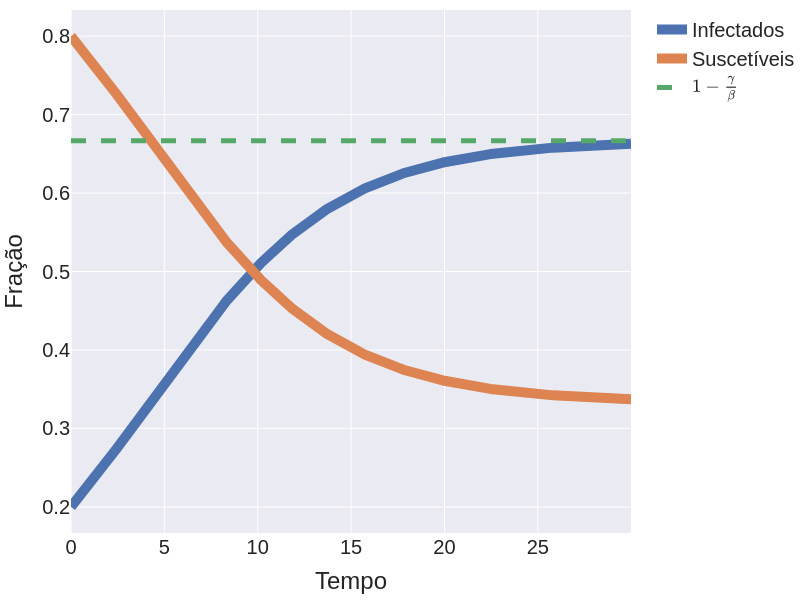
\includegraphics[scale=0.4]{figuras/SIS_1.png}
   \caption*{Gráfico que apresenta a evolução da infecção de um modelo 
   SIS com $I(0) = 0.2$, $\overline{\beta} = 0.3$ e $\overline{\gamma} = 0.1$. Nele existe convergência para equilíbrio estável no modelo SIS, com $\overline{\beta} > \overline{\gamma}$. Para $t \rightarrow \infty$, as frações de infectados e suscetíveis estabilizam em $1 - \frac{\overline{\gamma}}{\overline{\beta}}$ e $\frac{\overline{\gamma}}{\overline{\beta}}$ respectivamente, indicando persistência da doença em um horizonte infinito.\\Fonte: Autor.}
   \label{SIS}
\end{figure}


\begin{figure}[H]
  \centering
  \captionsetup{font=normalsize,skip=1pt,singlelinecheck=on,labelsep=endash}
  \caption{Modelo SIS}
  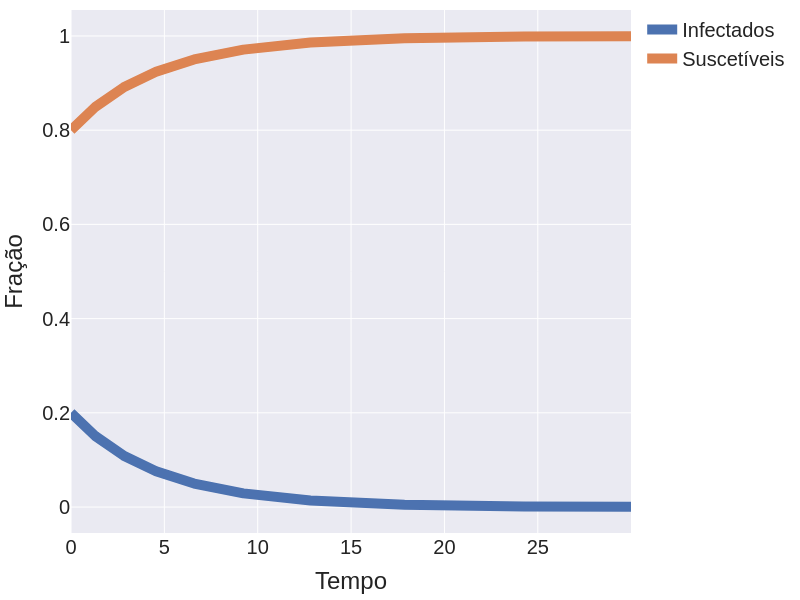
\includegraphics[scale=0.4]{figuras/SIS_2.png}
  \captionsetup{font=small,position=below,skip=-1pt}
   \caption*{Gráfico que apresenta a evolução da infecção de um modelo SIS com $I(0) = 0.2$, $\overline{\gamma} = 0.3$ e $\overline{\beta} = 0.1$. Caso $\overline{\beta} < \overline{\gamma}$, com a taxa de recuperação maior que a taxa de infecção, para $t \rightarrow \infty$, o número de infectados se aproxima de zero e o de suscetíveis se aproxima de um, indicando a erradicação da doença.\\Fonte: Autor.}
   \label{SIS_2}
\end{figure}

\subsection{Modelo SIR}


Por fim o último dos modelos básicos para o estudo de infecções é inspirado por doenças que após a infecção o indivíduo deixa de ser infectado, contudo, não pode ser infectado novamente, isso pode ter a interpretação de que o indivíduo ganhou imunidade ou morreu.
Esse
modelo é o SIR (suscetível, infectado e removido) na qual adiciona um novo compartimento R, conforme esquematização da Figura~\ref{img:SIR_}. Um exemplo de doença que pode ser modelada é a catapora no qual um indivíduo após infectado fica imune à enfermidade.

\begin{figure}[ht]
  \centering
  \captionsetup{font=normalsize,skip=0.8pt,singlelinecheck=on,labelsep=endash}
  \caption{Esquematização do Modelo Susceptível-Infectado-Removido de contágio.} 
  \begin{tikzpicture}

    \draw[->] (2,2.5) -- node[above] {$\overline{\beta}$} (3.9,2.5) ;
    \draw[->] (6.1,2.5) -- node[above] {$\overline{\omega}$} (7.9,2.5) ;
    
    \draw[rounded corners,drop shadow, fill=ninfect,draw=border, ultra thick] (0,2) rectangle (2,3)node[pos=.5,text= white,font=\fontsize{20}{20}\selectfont]  {$S$};
    
    \draw[rounded corners,drop shadow, fill=infect,draw=border, ultra thick](4, 2) rectangle (6,3) node[pos=.5,text= white,font=\fontsize{20}
    {20}\selectfont]  {$I$};
    \draw[rounded corners,drop shadow, fill=infect,draw=border, ultra thick](8, 2) rectangle (10,3) node[pos=.5,text= white,font=\fontsize{20}
    {20}\selectfont]  {$R$};
  \end{tikzpicture}
  \label{img:SIR_}
\end{figure}

O modelo SIR pode ser descrito pelas equações
\begin{align}
\frac{dS}{dt} &= -\overline{\beta} \cdot S \cdot I\\
\frac{dI}{dt} &= +\overline{\beta} \cdot S \cdot I- \overline{\omega} \cdot I\\
\frac{dR}{dt} &= +\overline{\omega} \cdot I\\
S +I+ R &= 1,
\label{SIR}
\end{align}
com $I(0) = I_0$, $R(0) = 0$ e $S(0) = S_0$ e $\overline{\omega}$ a taxa de remoção. Diferente dos modelos anteriores, esse não tem solução analítica para a equação diferencial acoplada precisando de uma solução usando métodos computacionais, contudo ainda é possível extrair análises a partir dessas equações. A partir da equação $\frac{dI}{dt}$ e igualando ela a zero existe um ponto crítico de máximo em $S = \frac{\overline{\omega}}{\overline{\beta}}$ que não aparecia nos modelos anteriores, enquanto $S > \frac{\overline{\omega}}{\overline{\beta}}$ o modelo apresenta numa fase endêmica, na qual o número de infectados cresce até chegar no ponto crítico, quando $S < \frac{\overline{\omega}}{\overline{\beta}}$ o número de infectados decresce até chegar no final da endemia. Esse valor crítico é chamado de número ou taxa de reprodutibilidade basal $R_0$ que representa o número médio de pessoas que são infectadas por um único indivíduo. 

\begin{figure}[H]
  \centering
  \captionsetup{font=normalsize,skip=1pt,singlelinecheck=on,labelsep=endash}
  \caption{Modelo SIR}
  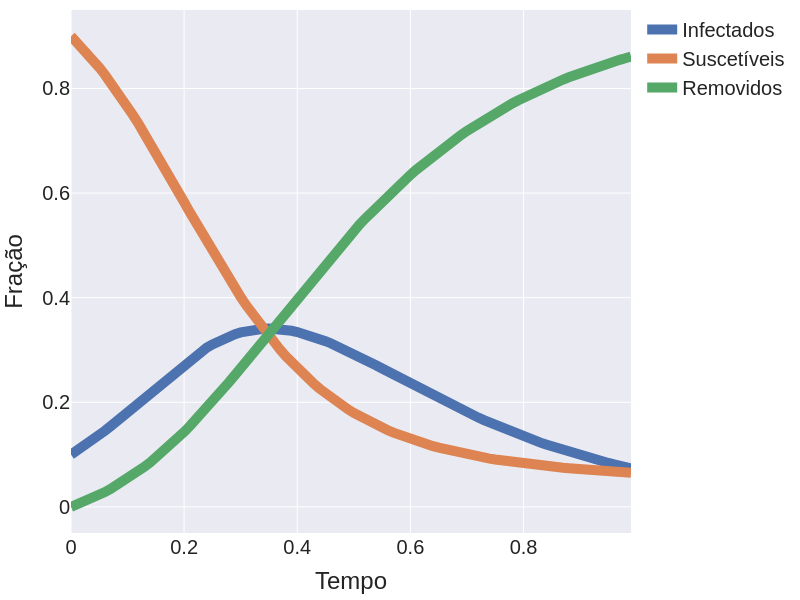
\includegraphics[scale=0.5]{figuras/SIR.png}
  \captionsetup{font=small,position=below,skip=-1pt}
   \caption*{Gráfico que apresenta a evolução da infecção de um modelo SIR com $I(0) = 0.2$,$S(0) = 0.8$, 
   $R(0) = 0$, $\overline{\omega} = 0.4$ e $\overline{\beta} = 1.2$. É mostrado existe um ponto de máximo de I(t), esse gráfico é bastante sensível aos parâmetros e seu comportamento pode mudar bastante com a alteração deles.  \\Fonte: Autor.}
   \label{img:SIR}
\end{figure}

\subsection{Modelos em Redes}

%PIF17042024 Acho que esta sub-seção precisa mais referências: a área de difusão de doenças em redes é muito ampla.
% Citar sobre outras modelagens em Redes

Toda a modelagem descrita anteriormente foi apresentada no contexto de equações diferenciais, porém ela tem as suas limitações como discutido anteriormente, contudo elucidam bem sobre como é feita esse tipo de modelagem. No contexto de redes complexas existem duas formas de construir a 
modelagem~\cite{networks}: 
de tempo contínuo ou de tempo discreto. 
Por exemplo, num modelo SI 
cada nó vai receber um rótulo descrevendo em qual compartimento ele está. No caso de tempo discreto um nó
$\nu$ 
no compartimento S tem uma
probabilidade $p = (1 - \beta)^{k^I_\nu}$ de não ser contaminado, na qual $\beta$ é diferente do que aparece nas equações diferenciais, enquanto no modelo de redes ele é uma probabilidade associada ao indivíduo, na modelagem por equações diferenciais é algo médio para todo o sistema, isso se aplica também ao $\gamma$ e $\omega$ e $k_\nu^I$ é o número de vizinhos de $\nu$ que estão no estágio $I$. Portanto, a probabilidade de ser contaminado por pelo menos um nó é de
\begin{equation}
    p_\nu = 1 - (1 - \beta)^{k^I_\nu}.
\end{equation}
Uma vez calculada a probabilidade de contágio, pode-se decidir se o vértice passará ao estado I, em cujo caso muda-se o próximo estado do vértice para I. Ou seja, depois de uma interação no modelo na qual passa uma unidade de tempo (depende da unidade de $\beta$) os nós suscetíveis 
têm 
probabilidade $p_i$ de serem contaminados, por isso é chamado de tempo discreto. No caso do modelo SIR ou SIS, existe uma probabilidade $\gamma$ ou $\omega$ dele sair do estado infectado. Contudo, essa probabilidade não depende dos seus vizinhos, então cada nó que esteja infectado tem uma probabilidade $\gamma$ ou $\omega$ de depois de uma unidade de tempo de mudar de estágio. O Algoritmo \ref{algoritmo:discreto} mostra um pseudo-código de como funciona para o caso discreto o modelo SIS.

\begin{algorithm}[htbp]
   \caption{Algoritmo caso discreto do modelo SIS}
   \label{algoritmo:discreto}
   \SetKwInOut{Input}{Input}
\Input{$G(\mathpzc{N} ,\mathpzc{L})$: rede.}
\Input{$random()$: função que retorna um número ao acaso em $(0,1)$.}

   \For{$\nu_i \in \mathpzc{N}$}{
      $\mathrm{estado}[i] \gets$ Inicialização de estados; \tcp{S ou I}
   }
   $t \gets 0$\\
   \While{$t \leq tempo$}{
      \For{$\nu_i \in \mathpzc{N}$}{ 
         \eIf{$\mathrm{estado}[i] = S$}{
            $\mathrm{num\_inf}\gets 0$\\
            \For{$\nu_j \in \eta(\nu_i)$}{
                \If{$\mathrm{estado}[j] = I$}{
                    $\mathrm{num\_inf}\gets \mathrm{num\_inf}+1$\\
                }
            }
            $p \gets 1 - (1 - \beta)^{\mathrm{num\_inf}}$\\
            
            \If{$random() < p$}{
               $\mathrm{estado}[i] \gets I$\\
            }
         }{
            \If{$random() < \gamma$}{
               $\mathrm{estado}[i] \gets S$\\
            }
         }
      }
      $t \gets t + 1$\\
   }
\end{algorithm}

Para tempo contínuo no modelo SI,tradicionalmente , cada nó tem um tempo 
$T_{\nu}^{s\rightarrow i} \sim \mathrm{Exp}(k_\nu^I\beta)$ (distribuição exponencial com parâmetro $k_\nu^I\beta$) para ser contaminado,
com $k_\nu^I = |I\cap \eta(\nu)|$ (contudo há estudos com tempos não exponenciais \cite{feng2007epidemiological}). Portanto, o tempo $\Delta t$ para a próxima atualização na rede segue uma distribuição exponencial com parâmetro a soma dos parâmetros de cada variável
$\Delta t \sim \mathrm{Exp}(\sum_{\nu \in S}k_\nu^I\beta)$,
pois o mínimo entre várias variáveis exponenciais independentes segue uma distribuição exponencial com a soma dos parâmetros.

A escolha do nó a ser atualizado é feita a partir do cálculo de 
$M = \sum_{\nu \in S}k_\nu\beta$.
Seja $S = \{\mu_1,\mu_2,\cdots,\mu_{|S|}\}$ uma ordem do conjunto de nós suscetíveis. Assim é gerado um valor $r$ aleatório entre 0 e 1, o nó $\mu_j$ a ser atualizado é primeiro vértice tal que $\sum_{i=1}^{j}k_{\mu_i}^I\beta \geq r\cdot M$. Para modelos como SIS e SIR segue a mesma ideia, sem considerar os vizinhos, o tempo para mudar de estágio é $T_{\nu}^{i\rightarrow s} \sim \mathrm{Exp}(\gamma)$ ou $T_{\nu}^{i\rightarrow r} \sim \mathrm{Exp}(\omega)$, agora $M$ é calculado com a soma de $\sum_{\nu \in S}k_\nu^I\beta+ \sum_{\nu \in I}\gamma$ ou de $\sum_{\nu \in S}k_\nu^I \beta+ \sum_{\nu \in I}\omega$ e assim o tempo que passa é $\Delta t \propto \mathrm{Exp}(M)$ e o nó escolhido é tal que a soma de todas as taxas até ele seja maior que $r\cdot M$~\cite{Gillespie1976}. O Algoritmo \ref{algoritmo:continuo} mostra um pseudo-código de como funciona para o caso contínuo o modelo SIS.


\begin{algorithm}[htbp]
   \caption{Algoritmo caso contínuo do modelo SIS}
   \label{algoritmo:continuo}
   \SetKwInOut{Input}{Input}
\Input{$G(\mathpzc{N} ,\mathpzc{L})$: rede.}
\Input{$random()$: função que retorna um número ao acaso em $(0,1)$.}
\Input{$exp(\lambda)$: função que retorna um número aleatório com distribuição exponencial de parâmetro $\lambda$.}
   \For{$\nu \in\mathpzc{N}$}{
      \tcp{Inicialização de estados}
      $S \gets S\cup \{\nu\}$ ou  $I \gets I\cup \{\nu\}$
   }
   $t \gets 0$\\
   \While{$t \leq tempo$}{
      $M \gets 0$\\
      \tcp{Os nós são visitados numa ordem fixa}
      \For{$\nu_i \in \mathpzc{N}$}{
         \eIf{$\nu_i \in S$}{
            $k_{\nu_i}^I \gets |I\cap \eta(\nu_i)|$\\
            $\mathrm{rate}[i] \gets k_\nu^I \cdot \beta$\\
         }{
            $\mathrm{rate}[i] \gets \gamma$\\
         }
         $M \gets M + \mathrm{rate}[i]$\\
      }
      $t \gets t + exp(M)$\\
      $\Delta \gets random() \cdot M$\\
      $m \gets 0$\\
      $i \gets 0$\\
      \While{$m \leq \Delta$}{
         $i \gets i + 1$\\
         $m \gets m + \mathrm{rate}[i]$\\
      }
      \eIf{$\nu_i \in S$}{
         $I \gets I\cup\{\nu_i\}$\\
         $S \gets S\setminus\{\nu_i\}$\\
      }{
         $S \gets S\cup\{\nu_i\}$\\
         $I \gets I\setminus\{\nu_i\}$\\
      }
   }
\end{algorithm}

	%\chapter{Metodologia}

\section{Coleta de Dados}

A utilização de Redes Complexas como ferramenta de modelagem para estudos sobre a Covid-19 é intuitiva, pois o espalhamento das epidemias ocorre através de complexas redes de interações humanas. Para a implementação dessa abordagem, é essencial dispor de dados sobre redes de contágio que incluam informações relevantes para a análise, como idade, tempo de contato, pertencimento a grupos de risco, entre outros aspectos.

Entretanto, não é fácil encontrar um banco de dados tão completo e não enviesado pela recente pandemia. Em 2008, visando o estudo da pandemia de influenza, a Comissão Europeia criou o projeto chamado POLYMOD~\cite{POLYMOD} que tinha o intuito da coleta de dados para entender quais seriam os padrões de contatos da Europa~\cite{Mossong2008}. Apoiado nesse estudo, pesquisas posteriores se inspiraram no formato do POLYMOD~\cite{Belga2009,Belga2010,China,France,HongKong,Peru,Russia,Thailand,Vietnam,Zambia,Zimbabwe}. Essa pesquisa foi feita baseada em um questionário de maio de 2005 até setembro de 2006 em 8 diferentes países da Europa a partir de ligações aleatórias ou entrevistas presenciais. Os participantes da pesquisa foram recrutados de forma a serem amplamente representativos de toda a população em termos de distribuição geográfica, idade e sexo e houve uma super-amostragem para crianças e adolescentes.

 Ao final do dia a pessoa teria que preencher o diário anotando sobre informações pessoais, ambiente (escola, trabalho, casa, ...) e as pessoas na qual teve contato de curto alcance no dia, a idade aproximada (ou exata) dessas pessoas, duração da conversa, frequência na qual têm contato, dentre outras informações. Caso o participante fosse empregado, ele teria que informar qual a média de contatos no seu trabalho, caso fosse maior que 20 então os contatos que seriam anotados no diário seriam os não profissionais. 

Apesar dos dados obtidos a partir do estudo POLYMOD, é crucial notar que este não constrói uma rede de conexões entre os participantes. Tal limitação é inerente à metodologia adotada pelo estudo, que se baseia em discagem e entrevistas
aleatórias para coleta de informações. A escolha por esse método implica que as conexões entre os participantes não são mapeadas diretamente na forma de uma rede interconectada. A rede gerada pelos dados seria aproximadamente formada por vários grafos estrelas desconectados em que os nós centrais da estrela são os participantes das entrevistas. Portanto, para ser possível formar uma rede e utilizar os dados anteriores é necessário um modelo adequado que leve em consideração a distribuição de graus e a idade. Um modelo muito utilizado na literatura é o \textit{stochastic block model} (SBM) \cite{SBM} na qual cada nó seria separado em um bloco e os nós pertencentes a cada bloco seriam conectados com probabilidade $p_{B_\nu,B_\mu}$, na qual $B_\nu$ é o bloco de $\nu$. A principal desvantagem dessa abordagem é que a rede gerada apresenta uma característica média não resgatando, por exemplo, a distribuição de graus dos dados. \citeonline{klise2022prioritizing} apresenta uma outra forma de construir a rede na qual separa a rede em camadas relacionadas aos locais onde os indivíduos visitam (casa, escola ou trabalho) entretanto para a base de dados do POLYMOD isso não é possível pois não se tem noção da totalidade das redes.

\section{Modelo de Formação de Redes Proposto}

Para evitar esse problema~\cite{Manzo2020} propõe um modelo para formação de uma rede baseado 
no modelo de configuração para um problema similar. A partir dos dois dias de entrevista é calculado a média de contatos por dia de cada pessoa (arredondado para cima) e utiliza o Modelo de Configuração para a formação de uma Rede Sintética. No entanto, o modelo de formação de redes gera um agrupamento médio limitado e ele é muito importante na suavização de epidemias~\cite{Block2020}. Nesse sentido, 
Manzo e Rijt propõe que antes de ser excluído um dado nó do Modelo de Configuração (Algoritmo \ref{alg:manzo}), passamos por cada
par de vizinhos dele e os conectamos entre si com uma probabilidade $p$. Ou seja:

\begin{enumerate}
  \item Quando um dado nó 
  $\nu$
   atinge o grau requerido pelo MC são selecionados todos os vizinhos 
    $\eta(\nu)$;
    
  \item São escolhidos dois nós aleatoriamente
  $\mu,\zeta\in \eta(\nu)$ 
  e são conectados com probabilidade $p$;
  \item Se a ligação existir conectamos e salvamos para que ela não se repita no MC, caso contrário salvamos para que ela não se repita nesse algoritmo. Por fim também reduzimos em 1 o valor de $\kappa_\mu$ e $\kappa_\zeta$,
se a ligação entre $\mu$ e $\zeta$ for adicionada na rede;
  \item Repetimos 2 até que todas as ligações possíveis sejam testadas e o algoritmo termina para dar continuidade ao MC.
\end{enumerate}

\begin{algorithm}[htbp]
   \caption{Implementação de Manzo e van Rijt}
   \label{alg:manzo}
   \SetKwInOut{Input}{Input}
\Input{$G(\mathpzc{N} ,\mathpzc{L})$: rede já construída}
\Input{$\mathpzc{L}_\mathrm{test}$: possíveis ligações já testadas \tcp{Não são testadas duas vezes.}} 
\Input{$random()$: função que retorna um número ao acaso em $(0,1)$.}

   \For{$\nu\in \mathpzc{N}$}{
      \For{$\mu \in \eta(\nu)$}{
         \For{$\zeta \in \eta(\nu)\setminus\{\mu\}$ }{
            \If{$(\kappa_\zeta \neq 0)$ 
            $\mathbf{and }$ $(\kappa_\mu \neq 0)$}{
             \If{(random() <= $p)$}{
              \If{$(\mu,\zeta) \not\in \mathpzc{L}\cup \mathpzc{L}_\mathrm{test}$}{
                     $\mathpzc{L} \gets \mathpzc{L}\cup\{(\mu,\zeta)\}$ \tcp{Essa matriz vem do MC}
                     $\kappa_\mu \gets \kappa_\mu - 1$\\
                     $\kappa_\zeta \gets \kappa_\zeta - 1$\\
                  }
               }{
                  $\mathpzc{L}_\mathrm{test} \gets \mathpzc{L}_\mathrm{test}\cup\{(\mu,\zeta)\}$
               }
            }
         }
      }
   }
\end{algorithm}



\begin{figure}[H]
  \centering
  \captionsetup{font=normalsize,skip=0.8pt,singlelinecheck=on,labelsep=endash}
  \caption{Ilustração do Modelo de Manzo}
  \begin{tikzpicture}[make origin horizontal center of bounding box]
    %Values
    \def\xa{2};
    \def\ya{sqrt(4-sqrt(\xa))}

    \def\xc{0.5};
    \def\yc{sqrt(4-sqrt(\xc))};

    \def\xb{0.5};
    \def\yb{sqrt(4-sqrt(\xb))};

    \def\xd{1.5};
    \def\yd{sqrt(4-sqrt(\xd))};

    \def\xe{1.3};
    \def\ye{sqrt(4-sqrt(\xe))};

    \draw[black, thick] (0,0) -- ($\xa*(1,0) + \ya*(0,1)$);

    \draw[black, thick, dotted]($\xa*(1,0) + \ya*(0,1)$) -- ($\xa*(0.5,0) + \ya*(0,0.01)$);

    
    \draw[black, thick] (0,0) -- ($\xb*(1,0) + \yb*(0,1)$);
    \draw[black, thick, dotted] ($\xb*(1,0) + \yb*(0,1)$) -- ($\xb*(1,0) + \yb*(0,1.5)$);
    \draw[black, thick, dotted] ($\xb*(1,0) + \yb*(0,1)$) -- ($\xa*(1,0) + \ya*(0,1)$);
    \draw[black, thick, dotted] ($\xb*(1,0) + \yb*(0,1)$) -- ($\xc*(1,0.5) + \yc*(0.3,0.5)$);
    \draw[black, thick, dotted] ($\xb*(1,0) + \yb*(0,1)$) -- ($\xc*(1,0.5) + \yc*(-0.3,0.5)$);

    \draw[black, thick] (0,0) -- ($\xc*(1,0) + \yc*(0,-1)$);
    \draw[black, thick, dotted] ($\xc*(1,0) + \yc*(0,-1)$) -- ($\xa*(0.7,0) + \ya*(0,0.01)$);
    \draw[black, thick, dotted] ($\xc*(1,0) + \yc*(0,-1)$) -- ($\xc*(-1.5,0) + \yc*(0,-1)$);
    

    \draw[black, thick] (0,0) -- ($\xd*(-1,0) + \yd*(0,-1)$);
    \draw[black, thick, dotted] ($\xd*(-1,0) + \yd*(0,-1)$) -- ($\xd*(-1,0) + \yd*(0,0.01)$);
    \draw[black, thick, dotted] ($\xd*(-1,0) + \yd*(0,-1)$) -- ($\xd*(-1.8,0) + \yd*(0,-1)$);

    \draw[black, thick] (0,0) -- ($\xe*(0,1) + \ye*(-1,0)$);

    % Nós

    \draw[black, fill=white, anchor=center] (0,0) circle [radius=0.25] node {3};
    \draw[black, fill=white] ($\xc*(1,0) + \yc*(0,1)$) circle [radius=0.25] node {5};
    \draw[black, fill=white] ($\xe*(0,1) + \ye*(-1,0)$) circle [radius=0.25] node {0};
    \draw[black, fill=white] ($\xd*(-1,0) + \yd*(0,-1)$) circle [radius=0.25] node {80};
    \draw[black, fill=white] ($\xb*(1,0) + \yb*(0,-1)$) circle [radius=0.25] node {32};
    \draw[black, fill=white] ($\xa*(1,0) + \ya*(0,1)$) circle [radius=0.25] node {18};
    \node at (0,3) {$p = 0$};
  \end{tikzpicture}
  \begin{tikzpicture}[make origin horizontal center of bounding box]
    %Values
    \def\xa{2};
    \def\ya{sqrt(4-sqrt(\xa))}

    \def\xc{0.5};
    \def\yc{sqrt(4-sqrt(\xc))};

    \def\xb{0.5};
    \def\yb{sqrt(4-sqrt(\xb))};

    \def\xd{1.5};
    \def\yd{sqrt(4-sqrt(\xd))};

    \def\xe{1.3};
    \def\ye{sqrt(4-sqrt(\xe))};

    \draw[black, thick] (0,0) -- ($\xa*(1,0) + \ya*(0,1)$);

    \draw[black, thick, dotted]($\xa*(1,0) + \ya*(0,1)$) -- ($\xa*(0.5,0) + \ya*(0,0.01)$);

    
    \draw[black, thick] (0,0) -- ($\xb*(1,0) + \yb*(0,1)$);
    \draw[black, thick, dotted] ($\xb*(1,0) + \yb*(0,1)$) -- ($\xb*(1,0) + \yb*(0,1.5)$);
    \draw[black, thick] ($\xb*(1,0) + \yb*(0,1)$) -- ($\xa*(1,0) + \ya*(0,1)$);
    \draw[black, thick, dotted] ($\xb*(1,0) + \yb*(0,1)$) -- ($\xc*(1,0.5) + \yc*(0.3,0.5)$);
    \draw[black, thick, dotted] ($\xb*(1,0) + \yb*(0,1)$) -- ($\xc*(1,0.5) + \yc*(-0.3,0.5)$);

    \draw[black, thick] (0,0) -- ($\xc*(1,0) + \yc*(0,-1)$);
    \draw[black, thick, dotted] ($\xc*(1,0) + \yc*(0,-1)$) -- ($\xa*(0.7,0) + \ya*(0,0.01)$);
    %\draw[black, thick, dotted] ($\xc*(1,0) + \yc*(0,-1)$) -- ($\xc*(-1.5,0) + \yc*(0,-1)$);
    

    \draw[black, thick] (0,0) -- ($\xd*(-1,0) + \yd*(0,-1)$);
    \draw[black, thick] ($\xd*(-1,0) + \yd*(0,-1)$) -- ($\xc*(1,0) + \yc*(0,-1)$);
    \draw[black, thick, dotted] ($\xd*(-1,0) + \yd*(0,-1)$) -- ($\xd*(-1.8,0) + \yd*(0,-1)$);

    \draw[black, thick] (0,0) -- ($\xe*(0,1) + \ye*(-1,0)$);


    \draw[black, fill=white, anchor=center] (0,0) circle [radius=0.25] node {3};
    \draw[black, fill=white] ($\xc*(1,0) + \yc*(0,1)$) circle [radius=0.25] node {5};
    \draw[black, fill=white] ($\xe*(0,1) + \ye*(-1,0)$) circle [radius=0.25] node {0};
    \draw[black, fill=white] ($\xd*(-1,0) + \yd*(0,-1)$) circle [radius=0.25] node {80};
    \draw[black, fill=white] ($\xb*(1,0) + \yb*(0,-1)$) circle [radius=0.25] node {32};
    \draw[black, fill=white] ($\xa*(1,0) + \ya*(0,1)$) circle [radius=0.25] node {18};
    \node at (0,3) {$p = 0.5$};
  \end{tikzpicture}
  \begin{tikzpicture}[make origin horizontal center of bounding box]
    \def\xa{2};
    \def\ya{sqrt(4-sqrt(\xa))}

    \def\xc{0.5};
    \def\yc{sqrt(4-sqrt(\xc))};

    \def\xb{0.5};
    \def\yb{sqrt(4-sqrt(\xb))};

    \def\xd{1.5};
    \def\yd{sqrt(4-sqrt(\xd))};

    \def\xe{1.3};
    \def\ye{sqrt(4-sqrt(\xe))};

    \draw[black, thick] (0,0) -- ($\xa*(1,0) + \ya*(0,1)$);

    
    \draw[black, thick] (0,0) -- ($\xb*(1,0) + \yb*(0,1)$);
    \draw[black, thick, dotted] ($\xb*(1,0) + \yb*(0,1)$) -- ($\xb*(1,0) + \yb*(0,1.5)$);
    \draw[black, thick] ($\xb*(1,0) + \yb*(0,1)$) -- ($\xa*(1,0) + \ya*(0,1)$);
    \draw[black, thick, dotted] ($\xb*(1,0) + \yb*(0,1)$) -- ($\xc*(1,0.5) + \yc*(0.3,0.5)$);

    \draw[black, thick] (0,0) -- ($\xc*(1,0) + \yc*(0,-1)$);
    

    \draw[black, thick] (0,0) -- ($\xd*(-1,0) + \yd*(0,-1)$);
    \draw[black, thick] ($\xd*(-1,0) + \yd*(0,-1)$) -- ($\xc*(1,0) + \yc*(0,-1)$);
    \draw[black, thick] ($\xd*(-1,0) + \yd*(0,-1)$) -- ($\xb*(1,0) + \yb*(0,1)$);
    \draw[black, thick] ($\xb*(1,0) + \yb*(0,-1)$) -- ($\xa*(1,0) + \ya*(0,1)$);

    \draw[black, thick] (0,0) -- ($\xe*(0,1) + \ye*(-1,0)$);

    % Nós

    \draw[black, fill=white, anchor=center] (0,0) circle [radius=0.25] node {3};
    \draw[black, fill=white] ($\xc*(1,0) + \yc*(0,1)$) circle [radius=0.25] node {5};
    \draw[black, fill=white] ($\xe*(0,1) + \ye*(-1,0)$) circle [radius=0.25] node {0};
    \draw[black, fill=white] ($\xd*(-1,0) + \yd*(0,-1)$) circle [radius=0.25] node {80};
    \draw[black, fill=white] ($\xb*(1,0) + \yb*(0,-1)$) circle [radius=0.25] node {32};
    \draw[black, fill=white] ($\xa*(1,0) + \ya*(0,1)$) circle [radius=0.25] node {18};
    \node at (0,3) {$p = 1$};
  \end{tikzpicture}
  \captionsetup{font=small}
  \caption*{Funcionamento do Modelo de Configuração, 
  escolhemos dois nós $i$ e $j$ aleatoriamente e os conectamos. O Algoritmo pode gerar várias topologias de redes, porém ainda limitadas pelas quantidades $\{k_i\}$ de graus impostas pelo MC.\\ Fonte: Elaborado pelo autor}
  \label{img:MC_P}
\end{figure}

O modelo é mostrado na Figura \ref{img:MC_P}, quando um dado nó  $\nu$ atinge o grau necessário para cada $\mu \in \eta(\nu)$ 
os nós são conectados entre si com uma probabilidade $p$ se o grau de
$\nu$ não tiver atingido seu valor. Para que esse algoritmo se adapte a problemática utilizaremos os dados do POLYMOD. A partir deles é possível construir a distribuição $\{k_\nu\}_{\nu\in\mathpzc{N}}$ de graus e $\{f_\nu\}_{\nu\in\mathpzc{N}}$ de faixas etárias. 

Nesse contexto será proposto uma nova atualização no MC, consideraremos o conjunto 
$\kappa_{\nu,f}$ de conexões de um dado nó 
$\nu$ de faixa etária $f_\nu$ com um nó de faixa etária $f$, 
as quais serão incorporadas ao modelo de configuração, resultando em uma atualização considerando as conexões por faixa etária na qual será chamado de Modelo de Configuração Ponderado (MCP). Para a implementação do MCP, é fundamental dispor tanto da distribuição empírica de graus quanto de uma matriz $M$ tal que 
$M_{f,a}$ registra a proporção média de conexões de um nó na faixa etária $f$ que vão pra faixa etária $a$. 
Adicionalmente, a distribuição $F_w$ das faixas etárias é calculada a partir de um conjunto de dados. O procedimento para a implementação do MCP é delineado nos passos seguintes:
\begin{enumerate}
    \item São criados $N$ nós na rede formando-se o conjunto $\mathpzc{N}$;
    \item Atribui-se a cada nó $\nu$ uma faixa etária $f_\nu$, seguindo uma distribuição empírica $F_w$;
    \item Com base nos dados coletados, são geradas $k_\nu$ meias arestas para cada nó $\nu\in\mathpzc{N}$, seguindo a distribuição de graus empírica da faixa etária $f_\nu$;
    \item Para cada nó $\nu$, o número de meias arestas que vão se conectar com cada faixa etária $a$, $\kappa_{\nu,f}$, é escolhido conforme a distribuição multinomial \textbf{Multi}($k_\nu, M_{f_\nu,:}$);
    \item Os nós são ordenados em ordem decrescente de grau, de acordo com a sequência $\{\kappa_\nu\}$, para facilitar a convergência do modelo;
    \item Para cada nó $\nu$,uma faixa etária $a$ que ainda tenha meias arestas $\kappa_{\nu,a}$ a serem conectadas. Um nó $\mu$ dessa faixa etária é escolhido aleatoriamente entre todos os nós, excluindo $\nu$, que não possuam conexões com $\nu$, e que ainda tenham meias arestas disponíveis $\kappa_{\mu,f_\nu}$ para estabelecer; 
    \item Para cada nó $\mu$ selecionado dessa maneira, estabelece-se uma conexão com $\nu$, e os contadores $\kappa_{\mu,f_\nu}$ e $\kappa_{\nu,a}$ são decrementados em 1;
    \item O processo termina para o nó $\nu$ quando $\kappa_{\nu,a} = 0$ para todas as faixas $a$ ou não exista um nó $\nu_j$ que possa ser selecionado como descrito no passo 6;
    \item Logo após deve-se utilizar o Algoritmo de Manzo e van de Rijt adaptado com parâmetro $p$ para incrementar o agrupamento;
    \item Os passos de 6 a 9 são repetidos para todos os nós da rede.
\end{enumerate}

O algoritmo \ref{alg:MCP} é o pseudocódigo do MCP. Assim como o modelo tradicional o MCP tem um agrupamento limitado e baixo, portanto será implementado uma nova versão do Modelo de 
Manzo e van de Rijt para o MCP. Contudo ele precisa fazer algumas alterações para poder se adaptar ao MCP que utiliza as faixas etárias. O algoritmo \ref{alg:MCP_MANZO} é um pseudo-código com o algoritmo adaptado utilizando as faixas etárias, ele é chamado logo após todas as ligações 
$\{\kappa_{\nu,a}\}$ serem colocadas ou quando todos os sítios forem checados.


\begin{algorithm}[H]
   \caption{Implementação do MCP}
   \label{alg:MCP}
   $\mathpzc{L} \gets \emptyset$\\
   \For{$\nu\in\mathpzc{N}$}{
        $f_\nu \gets $ segundo a distribuição $F_w$\\
        $k_\nu \gets $ segundo a distribuição empírica de graus da faixa $f_\nu$\\
       $\{\kappa_{\nu,:}\}\gets $ segundo a distribuição multinomial \textbf{Multi}($k_\nu, M_{f_\nu,:}$)\\
       lista[$f_\nu$] $\gets \text{lista}[f_\nu] \cup \{\nu\}$\\
   }
   $\text{ordem} \gets $ordenar(\{$\nu$\},\{$k_\nu$\}) \tcp{Ordena os nós por número de meias arestas, em ordem decrescente.}
   \For{$\nu \in \mathrm{ordem}$}{
        \For{a < tamanho($F_w$)}{
            embaralha(lista[f])\\
            \For{$\mu\in\mathrm{lista}[a]\setminus \{\nu\}$}{
                \If{$\left[\kappa_{\mu,f_\nu} \neq 0\right]$ \textbf{and}  $\left[(\nu,\mu) \not\in \mathpzc{L}\right]$}{
                    $\mathpzc{L} \gets \mathpzc{L}\cup\{(\nu,\mu)\}$\\
                    $\kappa_{\nu,a} \gets \kappa_{\nu,a} - 1$\\
                    $\kappa_{\mu,f_\nu} \gets \kappa_{\mu,f_\nu} - 1$\\
                }
                \lIf{$\kappa_{\nu,a} == 0$}{
                    \textbf{break}
                }
            }
            Manzo\_Rijt($\nu,p$)
        }
   }
\end{algorithm}

\begin{algorithm}[htbp]
   \caption{Implementação de Manzo e van Rijt - Adaptado}
   \label{alg:MCP_MANZO}
   \SetKwInOut{Input}{Input}
\Input{$\nu$: nó sob consideração}
\Input{$p$: probabilidade de conexão} 
\Input{$G(\mathpzc{N} ,\mathpzc{L})$: rede já construída}
\Input{$\mathpzc{L}_\mathrm{test}$: possíveis ligações já testadas \tcp{Não são testadas duas vezes.}} 
\Input{$random()$: função que retorna um número ao acaso em $(0,1)$.}

   \For{$\mu \in \eta(\nu)$}{
        \If{$\text{soma}(\kappa_{\mu,:}) \neq 0$}{
            $\text{lista\_vizinhos}[f_\mu] \gets \text{lista\_vizinhos}[f_\mu] \cup \{\mu\}$\\
        }
   }

   \For{$\mu \in \eta(\nu)$}{
        \For{a < tamanho($F_w$)}{
            embaralha(lista\_vizinhos[$f$])\\
            \For{$\zeta \in \mathrm{lista\_vizinhos}[a]\setminus \{v\}$}{
                \lIf{$\kappa_{\mu,a} == 0$}{
                        \textbf{break}
                }
                \If{$\kappa_{\zeta,f_\mu} \neq 0$}{
                     \If{(random() <= $p)$}{
                      \If{$(\mu,\zeta) \not\in \mathpzc{L}\cup \mathpzc{L}_\mathrm{test}$}{
                             $\mathpzc{L} \gets \mathpzc{L}\cup\{(\mu,\zeta)\}$ \tcp{Essa matriz vem do MC}
                             $\kappa_{\mu,a} \gets \kappa_{\mu,a} - 1$\\
                             $\kappa_{\zeta,f_\mu} \gets \kappa_{\zeta,f_\mu} - 1$\\
                          }
                       }{
                          $\mathpzc{L}_\mathrm{test} \gets \mathpzc{L}_\mathrm{test}\cup\{(\mu,\zeta)\}$
                       }
                }
            }
        }
   }
\end{algorithm}

\section{Modelo de Infecção para COVID-19}

Artigos~\cite{Liu2022,Xiang2021} apresentam vários tipos de modelos na qual a literatura se utilizou para modelar a infecção e é importante entender qual é o melhor balanceamento de variáveis para não ficar muito complexo ou muito simplificado. Neste sentido, o modelo a ser utilizado é o 
SEIHARDS~\cite{Eikenberry2020} como base para nossa primeira aproximação. Ao contrário do paradigma inicial, a consideração da faixa etária dos indivíduos foi incorporada, reconhecendo-se as variações na suscetibilidade e resposta imunológicas associadas à idade. Além disso, a variável referente ao uso de máscaras faciais não foi incluída na nossa formulação, pois a ênfase está na análise de outros elementos de intervenção, o modelo epidemiológico adotado baseia-se em redes e houve a inclusão da possibilidade de recidiva à suscetibilidade após recuperação. Ele é composto pelos estágios: Suscetíveis (\textbf{S}), Expostos (\textbf{E}), Infectados Sintomáticos (\textbf{I}), Hospitalizados (\textbf{H}), Infectados Assintomáticos (\textbf{A}), Recuperados (\textbf{R}) e Mortos (\textbf{D}) que são modelados da seguinte forma:

\begin{itemize}
  \item \textbf{Suscetível (S)}: o nó neste estágio pode ser infectado pelos seus vizinhos que estão no estágio \textbf{A} ou no estágio \textbf{E}, essa taxa será $\epsilon_S$ vezes o número de contatos que estão no estágio \textbf{E} somado $\epsilon_A$ vezes o número de contatos no estágio A resultando na Equação \ref{eq:lambda} e um exemplo ilustrado é a Figura \ref{img:figinfect}.
  \begin{equation}
    \Lambda_\nu = \frac{|\mu \in \eta(\nu)\cap E|\cdot \epsilon_S + |\mu \in \eta(\nu)\cap A|\cdot \epsilon_A}{\langle k \rangle}
    \label{eq:lambda}
  \end{equation}

  \begin{figure}[ht]
  \centering
  
  
  \captionsetup{font=normalsize,skip=0.8pt,singlelinecheck=on,labelsep=endash}
  \caption{Ilustração do cálculo da taxa para se tornar infectado.}

  
  \begin{tikzpicture}[make origin horizontal center of bounding box]
    %Values
    \def\xa{2};
    \def\ya{sqrt(4-sqrt(\xa))}

    \def\xc{0.5};
    \def\yc{sqrt(4-sqrt(\xc))};

    \def\xb{0.5};
    \def\yb{sqrt(4-sqrt(\xb))};

    \def\xd{1.5};
    \def\yd{sqrt(4-sqrt(\xd))};

    \def\xe{1.3};
    \def\ye{sqrt(4-sqrt(\xe))};

    \draw[black, thick] (0,0) -- ($\xa*(1,0) + \ya*(0,1)$);
    
    \draw[black, thick] (0,0) -- ($\xb*(1,0) + \yb*(0,1)$);

    \draw[black, thick] (0,0) -- ($\xc*(1,0) + \yc*(0,-1)$);
    
    \draw[black, thick] (0,0) -- ($\xd*(-1,0) + \yd*(0,-1)$);

    \draw[black, thick] (0,0) -- ($\xe*(0,1) + \ye*(-1,0)$);

    % Nós

    \draw[black, fill=ninfect, anchor=center] (0,0) circle [radius=0.25] node {S};
    \draw[black, fill=infect] ($\xc*(1,0) + \yc*(0,1)$) circle [radius=0.25] node {E};
    \draw[black, fill=infect] ($\xe*(0,1) + \ye*(-1,0)$) circle [radius=0.25] node {E};
    \draw[black, fill=infect] ($\xd*(-1,0) + \yd*(0,-1)$) circle [radius=0.25] node {A};
    \draw[black, fill=ninteract] ($\xb*(1,0) + \yb*(0,-1)$) circle [radius=0.25] node {H};
    \draw[black, fill=ninteract] ($\xa*(1,0) + \ya*(0,1)$) circle [radius=0.25] node {H};
    \node at (0,3) {$\Lambda = 2\cdot\epsilon_S +1\cdot\epsilon_A = 2\cdot0.5+1\cdot0.41 = 1.41\, \mathrm{dia}^{-1}$};
  \end{tikzpicture}
  

  \label{img:figinfect}
\end{figure}

  \item \textbf{Exposto (E)}: um nó é considerado exposto quando ele estava no estágio \textbf{S} e foi contaminado por alguém no estágio \textbf{E} ou \textbf{A}. Este estágio é para representar os indivíduos que estão na fase de incubação do vírus, isso faz com que eles possam contaminar os outros indivíduos por não saberem que têm a doença. Deste estágio, ele pode passar para o estágio \textbf{I} com uma probabilidade 
  $\alpha^f$%PIF 16/5
, dependente da faixa etária $f$, 
  ou para o estágio \textbf{A} com probabilidade (1 - $\alpha^f$) mas com a mesma taxa $\sigma$.%;
  
  \item \textbf{Infectado Sintomático (I)}: um nó neste estágio está infectado, porém ele não pode infectar outras pessoas. Isso é feito para modelar um indivíduo que está sentindo os sintomas e, por isso, foi isolado e não teria mais contato com outras pessoas. 
  Uma pessoa neste estágio tem probabilidade $\psi^f$ de se hospitalizar, neste caso o tempo até hospitalização segue uma taxa $\phi^f$. Caso não seja necessária a hospitalização, a taxa do tempo de recuperação de sintomáticos é dada por $\gamma_I$.%;

  \item \textbf{Hospitalizado (H)}: nele o nó continua sem a capacidade de contaminar outros nós. Nesse estágio ele tem uma probabilidade $\tau^f$ de ir para o compartimento Morto com taxa $\delta$ e uma (1 - $\tau^f$) de se recuperar com taxa $\gamma_H$;
  
  \item \textbf{Infectado Assintomático (A)}: a diferença deste estágio para o \textbf{I} é o fato de que ele pode infectar outras pessoas. Isso se deve ao fato de que se ele é assintomático então não tem conhecimento da doença por não sentir nenhum sintoma, portanto ele continua tendo seus contatos e também não tem risco de morte ou necessidade de ser hospitalizado. Um indivíduo neste estágio se recupera com uma taxa $\gamma_A$.%;
  
  \item \textbf{Recuperado (R)}: caso o nó não morra ele será considerado recuperado na qual consegue voltar a ser suscetível novamente com uma taxa $\chi$.%;
  
  \item \textbf{Morto (D)}: Por fim, neste estado o nó perde todas as conexões e é nele que serão contabilizadas quantas pessoas morreram para utilizarmos como uma das métricas de minimização.
  
\end{itemize}

Na Figura \ref{img:Contagio} está esquematizado como funciona a dinâmica de infecção, sem considerar a vacinação das pessoas. 
No modelo, é assumido que o tempo de transição entre os estados segue uma distribuição exponencial com o parâmetro descrito como um rótulo das arestas na Figura~\ref{img:Contagio}. Os valores de cada parâmetro estão indicados nas Tabelas \ref{tabela:taxas_transicao_adaptada} e \ref{tabela:probabilidades_transicao_adaptada}.
Estes valores foram obtidos de 2 formas: ou pela busca em artigos ou utilizando a base de dados do openDataSUS para Síndrome Respiratória Aguda Grave de 2020~\cite{openDataSUSs}, um portal brasileiro na qual existem dados de internações Covid-19 e outras doenças gripais. Para achar $1/\gamma_H$, $1/\phi$, foi calculado a partir da média da diferença do tempo de uma pessoa ter sido internada para o tempo que ela saiu do hospital ou morreu, já a probabilidade $\tau^f$ foi obtida calculando quantas pessoas em uma faixa etária morreram dado que tinham sido internadas. Ademais, pelo fato de que o openDataSUS é limitado aos dados de internações, tornou-se necessária a busca de mais dados em artigos científicos.

\begin{figure}[ht]
  \centering

  \captionsetup{font=normalsize,skip=0.8pt,singlelinecheck=on,labelsep=endash}
  \caption{Esquematização do Modelo SEIHARDS de contágio}
  \begin{tikzpicture}[scale=0.9, every node/.style={scale=0.9}]

    \draw[->] (2,2.5) -- node[fill=white] {$\Lambda_\nu$} (3.9,2.5) ;
    \draw[->] (6,3.0) -- node[above,rotate=32]{$\sigma$} (7.9,4);
    \draw[->] (6,3.0) -- node[below,rotate=32]{\color{azuul}$1 - \alpha^f$} (7.9,4);
    

    \draw[->] (6,2.0) -- node[above,rotate=-32]{$\sigma$} (7.9,1);
    \draw[->] (6,2.0) -- node[below,rotate=-32]{\color{azuul}$\alpha^f$} (7.9,1);
    \draw[->] (10,4) -- node[fill=white] {$\gamma_A$} (12,5);

    \draw[->] (10,1) -- node[above] {$\phi$} (11.95,1);
    \draw[->] (10,1) -- node[below] {\color{azuul}$\psi^f$} (11.95,1);
    \draw[->] (14,1.) -- node[below] {\color{azuul} $\tau^f$} (16,1.);
    \draw[->] (14,1.) -- node[above] {$\delta$} (16,1.);
    \draw[->] (13,1.5) -- node[above,rotate=90] {\small $\gamma_H$} (13,4.5);
    \draw[->] (13,1.5) -- node[below,rotate=90] {\color{azuul}\small $1 - \tau^f$} (13,4.5);
    \draw[->] (10,1.5) -- node[above,rotate=45] {\small $\gamma_I$} (12,4.5);
    \draw[->] (10,1.5) -- node[below,rotate=45] {\color{azuul}\small $1 - \psi^f$} (12,4.5);
    
    \draw[->]  (13,5.) parabola (1,3.1);
    
    \node[draw,fill = white,draw = white] at (6,4.5) {$\chi$};
    
    
    \draw[rounded corners,drop shadow, fill=ninfect,draw=border, ultra thick] (0,2) rectangle (2,3)node[pos=.5,text= white,font=\fontsize{20}{20}\selectfont]  {$S_i$};
    
    \draw[rounded corners,drop shadow, fill=infect,draw=border, ultra thick](4, 2) rectangle (6,3) node[pos=.5,text= white,font=\fontsize{20}
    {20}\selectfont]  {$E_i$};
    
    \draw[rounded corners,drop shadow, fill=infect,draw=border, ultra thick](8, 3.5) rectangle (10,4.5) node[pos=.5,text= white,font=\fontsize{20}
    {20}\selectfont]  {$A_i$};
    
    \draw[rounded corners,drop shadow, fill=ninteract,draw=border, ultra thick](8, 0.5) rectangle (10,1.5) node[pos=.5,text= white,font=\fontsize{20}
    {20}\selectfont]  {$I_i$};
    
    \draw[rounded corners,drop shadow, fill=ninteract,draw=border, ultra thick](12, 0.5) rectangle (14,1.5) node[pos=.5,text= white,font=\fontsize{20}
    {20}\selectfont]  {$H_i$};
    
    \draw[rounded corners,drop shadow, fill=ninteract,draw=border, ultra thick](16, 0.5) rectangle (18,1.5) node[pos=.5,text= white,font=\fontsize{20}
    {20}\selectfont]  {$D_i$};
    
    \draw[rounded corners,drop shadow, fill=ninteract,draw=border, ultra thick](12, 5.5) rectangle (14,4.5) node[pos=.5,text= white,font=\fontsize{20}
    {20}\selectfont]  {$R_i$};
    
  \end{tikzpicture}
  %PIF27092023
  \captionsetup{font=small}
  \caption*{Ilustração do Modelo SEIHARD. Os blocos em vermelho significam quem pode contaminar outros, os blocos em azul escuro mostra o compartimento ainda não infectado e em azul claro mostra o estágio na qual o indivíduo não interage mais com a rede. Os parâmetros em preto são as taxas e em verde escuro são as probabilidades de entrar no estágio.}
  \label{img:Contagio}
\end{figure}

\begin{table}[H]
    \captionsetup{width=13.5cm}
    \caption{Taxas de transição utilizadas no modelo SEIAHRDS.}
    \centering
    \begin{tabular}{crrrrrrrr}
        \toprule
        Parâmetro & Definição & Valor [dia\(^{-1}\)] & Notas \\
        \midrule
        \midrule
        \(\epsilon_E\) & Taxa de contágio Expostos & 0.500 & \(^{(1)}\) \\
        \(\epsilon_A\) & Taxa de contágio Assintomática & 0.410 & \(^{(2)}\) \\
        \(\sigma\) & Taxa E\(\rightarrow\)A, E\(\rightarrow\)I (incubação) & 0.196 & \(^{(1)}\) \\
        \(\gamma_A\) & Taxa de recuperação de Assintomáticos & 0.143 & \(^{(1)}\) \\
        \(\gamma_I\) & Taxa de recuperação de Sintomáticos & 0.143 & \(^{(1)}\) \\
        \(\gamma_H\) & Taxa de recuperação de Hospitalizados & 0.083 & \(^{(3)}\) \\
        \(\phi\) & Taxa I\(\rightarrow\)H & 0.144 & \(^{(3)}\) \\
        \(\delta\) & Taxa de Mortalidade de Hospitalizados & 0.073 & \(^{(3)}\) \\
        \(\chi\) & Taxa R\(\rightarrow\)S (imunidade post-Covid) & 0.025 & \(^{(4)}\) \\
        \bottomrule
    \end{tabular}
    \caption*{Fontes: \(^{(1)}\)~\cite{Eikenberry2020}; \(^{(2)}\)~\cite{SP}; \(^{(3)}\) calculados usando o openDataSUS; \(^{(4)}\)~\cite{Kirkcaldy2020}.}
    \label{tabela:taxas_transicao_adaptada}
\end{table}


Considerando agora a vacinação, serão utilizados os dados da vacina da Pfizer-BioNTech, que apresenta uma grande eficácia \cite{HadjHassine2021} e 
foi a primeira vacina a ser utilizada. 
Como as vacinas só se tornaram disponíveis depois que a COVID-19 já tinha se espalhado por todas as regiões, adotaremos a convenção de que os indivíduos serão vacinados quando a difusão da doença já tenha entrado em um regime estacionário e o número de infectados tenha se estabilizado. Ao chegar nesse ponto são vacinados uma fração $f$ dos nós e devido à característica da vacina apenas os indivíduos nos estágios Suscetível, Recuperados ou Assintomáticos de acordo com um dado critério de prioridade. 
Com a vacinação, os parâmetros $\epsilon_S$, $\epsilon_A$, $\Lambda_\nu$, $\alpha^f$, $\psi^f$, e $\tau^f$ que influenciam a velocidade de propagação da infecção e a probabilidade de assintomatismo são alterados. No modelo, as mortes estão associadas aos indivíduos que passam pelo estágio sintomático, e esses parâmetros são críticos para a minimização do impacto. As modificações ocorrem por meio da multiplicação da eficácia da vacina, e os novos valores estão detalhados na Tabela \ref{tabela:vacina_adaptada}.


\begin{table}[H]
    \captionsetup{width=13.5cm}
    \caption{Probabilidades de transição por faixa etária.}
    \centering
    \begin{tabular}{crrrrrrr}
        \toprule
        Parâmetro & Definição & 0 - 20 & 20 - 30 & 30 - 50 & 50 - 70 & \(\geq\) 70 & Notas \\
        \midrule
        \midrule
        \(\alpha^f\) & Prob. E\(\rightarrow\)I & 29.10\% & 37.40\% & 41.68\% & 39.40\% & 31.30\% & \(^{(1)}\) \\
        \(\psi^f\) & Prob. I\(\rightarrow\)H & 0.408\% & 1.040\% & 3.890\% & 9.980\% & 17.500\% & \(^{(2)}\) \\
        \(\tau^f\) & Prob. H\(\rightarrow\)D & 1.040\% & 1.330\% & 1.380\% & 7.600\% & 24.000\% & \(^{(3)}\) \\
        \bottomrule
    \end{tabular}
    \caption*{Fontes: \(^{(1)}\)~\cite{Jung2020}; \(^{(2)}\)~\cite{RochaFilho2022}; \(^{(3)}\) calculada usando o openDataSUS.}
    \label{tabela:probabilidades_transicao_adaptada}
\end{table}


\begin{table}[H]
    \captionsetup{width=13.5cm}
    \caption{Mudança de parâmetros ao vacinar um nó.}
    \centering
    \begin{tabular}{crr}
        \toprule
        Definição & Não Vacinado & Vacinado  \\
        \midrule
        \midrule
        Taxa de contágio Sintomática & \(\epsilon_S\) & \(0.058 \times \epsilon_S\)\\
        Taxa de contágio Assintomática & \(\epsilon_A\) & \(0.058 \times \epsilon_A\)\\
        Prob. E\(\rightarrow\)I & \(\alpha^f\) & \(0.346 \times \alpha^f\)\\
        Prob. I\(\rightarrow\)H & \(\psi^f\) & \(0.034 \times \psi^f\) \\
        Prob. H\(\rightarrow\)D & \(\tau^f\) & \(0.034 \times \tau^f\)\\
        \bottomrule
    \end{tabular}
    \caption*{Valores das eficácias e sua interferência nos parâmetros. Fonte:~\cite{Haas2021}.}
    \label{tabela:vacina_adaptada}
\end{table}


	%\chapter{Resultados}
\label{chap:resultados}

\subsection{Análise exploratória}

A partir da coleta de dados realizada pelo POLYMOD, o propósito é elucidar a estruturação das interconexões interpessoais e analisar as implicações decorrentes dessas relações visando uma modelagem em redes. Para isso cada indivíduo foi categorizado em 5 faixas etárias: [0,20) (jovens), [20,30) (jovens adultos), [30,50) (adultos), [50,70) (adultos \textit{seniors}) e maiores de 70 que representam os idosos; a distribuição de cada faixa etária é mostrada na Figura \ref{fig:freq}. Esta categorização reveste-se de relevância considerável, haja vista que a estimação dos parâmetros utilizados é viável com a categorização das idades. 

\begin{figure}[H]
    \centering

    \captionsetup{font=normalsize,skip=0.8pt,singlelinecheck=on,labelsep=endash}
    \caption{Faixas etárias no banco de dados POLYMOD}
    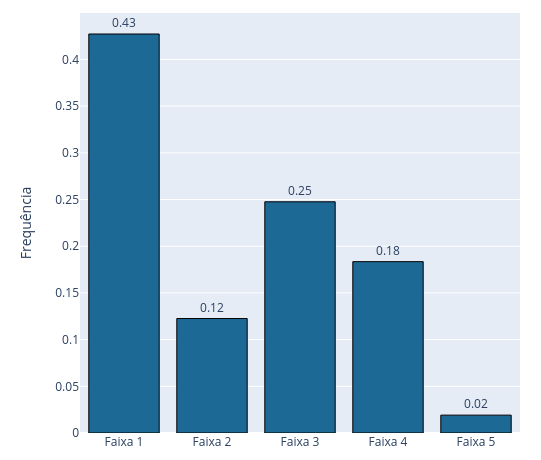
\includegraphics[scale= 0.5]{figuras/faixas_polymod-PIF.png}
        %PIF15102023
    %\captionsetup{font=small}
    \captionsetup{font=small,justification=justified}
    \caption*{Resultados da frequência de cada faixa etária no banco de dados POLYMOD, esse será um dos \textit{inputs} do modelo posteriormente.\\ Fonte: Autor.}

    \label{fig:freq}
\end{figure}

Com base nos dados obtidos, será realizada uma investigação para avaliar a duração, frequência e a presença de contato físico nos encontros em análise. A Figura \ref{fig:graficos} mostra os padrões dos contatos do POLYMOD; é possível ver que quanto mais frequente ou durável é o contato maior a chance dele ter contato físico.
Além disso, quanto mais frequente é o contato maiores as chances da conversa durar mais, por exemplo em contatos diários existe mais de 50\% de chance de que o contato dure mais que 1 hora. Por fim, o gráfico mais recente evidencia que, no ambiente domiciliar, a probabilidade de ocorrência de contato físico é significativamente maior, especialmente em áreas designadas para o lazer. Por contraste, no ambiente profissional, as chances são substancialmente menores, sendo considerado o cenário menos propenso a esse tipo de interação.

\begin{figure}[H]
    \centering
    \captionsetup{font=normalsize,skip=0.8pt,singlelinecheck=on,labelsep=endash}
    \caption{Probabilidade de contato físico}
    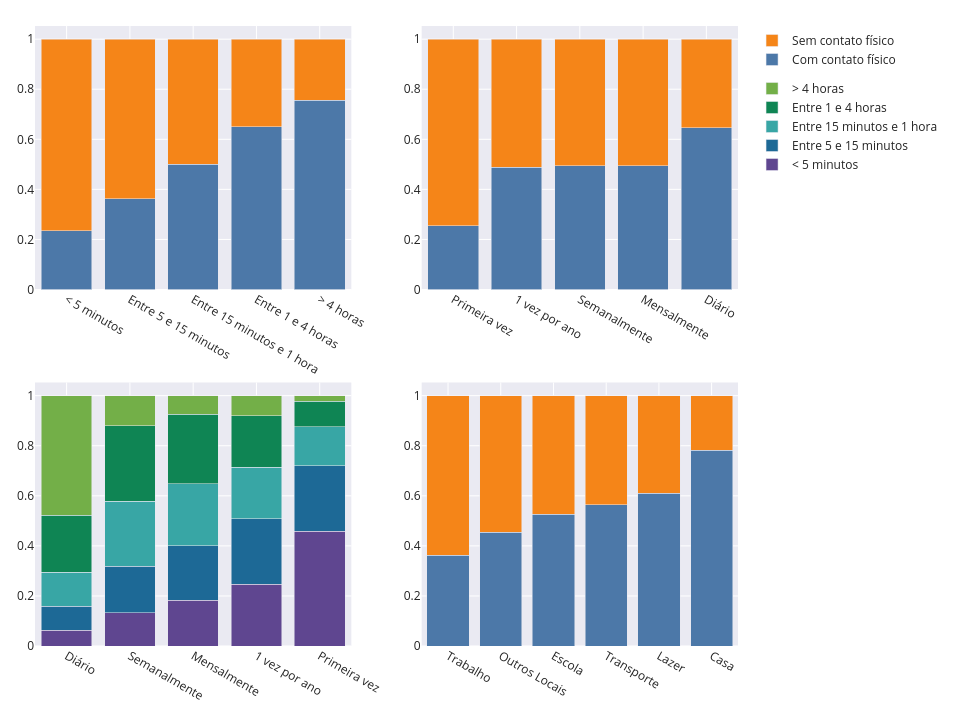
\includegraphics[scale= 0.45]{figuras/graficos-PIF.png}
\captionsetup{font=small,justification=justified}
    \caption*{Ilustra a relação entre a frequência e a duração dos contatos com a probabilidade de contato físico, mostrando que contatos mais frequentes e duradouros têm maior probabilidade de envolver contato físico. Além disso, o ambiente domiciliar apresenta maior probabilidade de contato físico, especialmente nas áreas de lazer, em comparação ao ambiente profissional, onde a probabilidade é consideravelmente menor. Todas as correlações são altamente significantes.\\ Fonte: Autor.}
    \label{fig:graficos}
\end{figure}


Um elemento importante que foi investigado foi como as idades influenciam nas conexões entre os indivíduos da rede. Na Figura \ref{fig:contatos_faixa} nota-se como é a distribuição de idades da pesquisa. Ao analisar a distribuição de ligações por faixa etária é percebido que seguem uma distribuição geométrica, que pode ser escrita como $P \propto (1 - p)^xp$ ou $P \propto e^{-\lambda x}(1 - e^\lambda)$. Na Figura \ref{fig:contatos_faixa} temos o estudo das distribuições como se fosse da segunda forma, no eixo das abscissas o grau e no eixo das ordenadas o logaritmo da probabilidade, com isso é encontrado uma reta com Mínimos Quadrados na qual o coeficiente angular é igual ao $\lambda$ e seu respectivo $R^2$. 

\begin{figure}[H]
    \centering
    \captionsetup{font=normalsize,skip=0.8pt,singlelinecheck=on,labelsep=endash}
    \caption{Influência das idades nas conexões}
    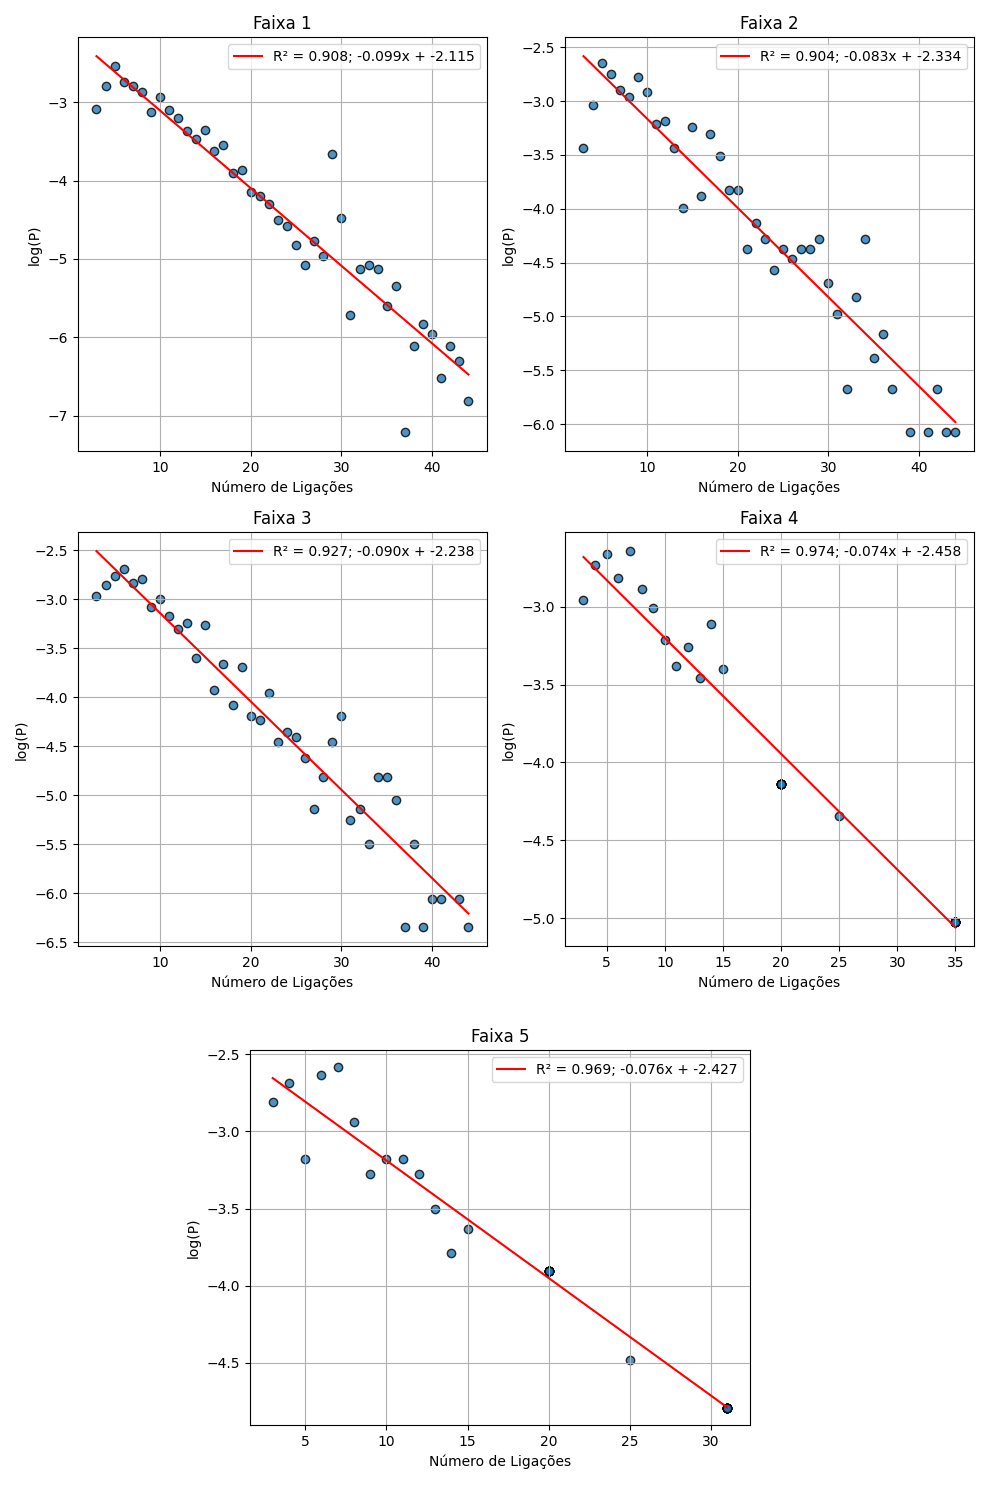
\includegraphics[scale= 0.3]{figuras/contatos_faixa.png}
    \captionsetup{font=small,justification=justified}
    \caption*{Ilustra a influência das idades nas 
    conexões da rede social, observando uma distribuição geométrica nas ligações por faixa etária.\\ Fonte: Autor.}
    \label{fig:contatos_faixa}
\end{figure}

A pesquisa também revela a relação entre a faixa etária de um indivíduo que preencheu o questionário e a distribuição de suas ligações. A Figura \ref{fig:heat} ilustra para cada faixa etária das linhas, a frequência relativa de conexões com as faixas etárias das colunas. Notavelmente, a faixa etária 3 apresenta a maior frequência de conexões, sendo composta majoritariamente por indivíduos que estão na fase produtiva da vida, muitas vezes já com família estabelecida. Em contraste, a última faixa etária demonstra a menor frequência de conexões, presumivelmente devido às dificuldades associadas a essa fase da vida.

\begin{figure}[H]
    \centering
    \captionsetup{font=normalsize,skip=0.8pt,singlelinecheck=on,labelsep=endash}
    \caption{Frequência média de conexões por faixa etária}
    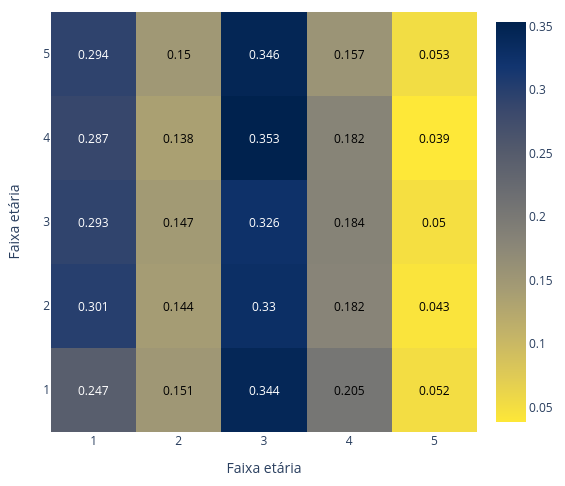
\includegraphics[scale= 0.5]{figuras/h-PIF.png}
    \captionsetup{font=small,justification=justified}
    \caption*{Mostra a frequência média de conexões por faixa etária, ressaltando que a faixa etária 3, associada à vida profissional e familiar, possui a maior frequência de conexões, enquanto a última faixa apresenta a menor frequência devido às dificuldades inerentes a essa fase da vida. \\Fonte: Autor}
    \label{fig:heat}
\end{figure}

Por último, a Figura \ref{fig:mediastd} apresenta duas matrizes de calor que ilustram a média e o desvio padrão do tempo de contato entre diferentes faixas etárias. A matriz da média mostra que as faixas etárias tendem a ter maior tempo de contato consigo mesmas e com faixas etárias adjacentes, com tempos decrescentes à medida que a diferença de idade aumenta. Notavelmente, a Faixa Etária 1 possui os maiores tempos médios de contato consigo mesma e com a Faixa Etária 2, enquanto os tempos são menores com as faixas etárias superiores e a Faixa Etária 4 apresenta contato elevado com a Faixa Etária 5.

\begin{figure}[H]
    \centering
    \captionsetup{font=normalsize,skip=0.8pt,singlelinecheck=on,labelsep=endash}
    \caption{Média e desvio-padrão dos tempos de contato entre faixas etárias}
    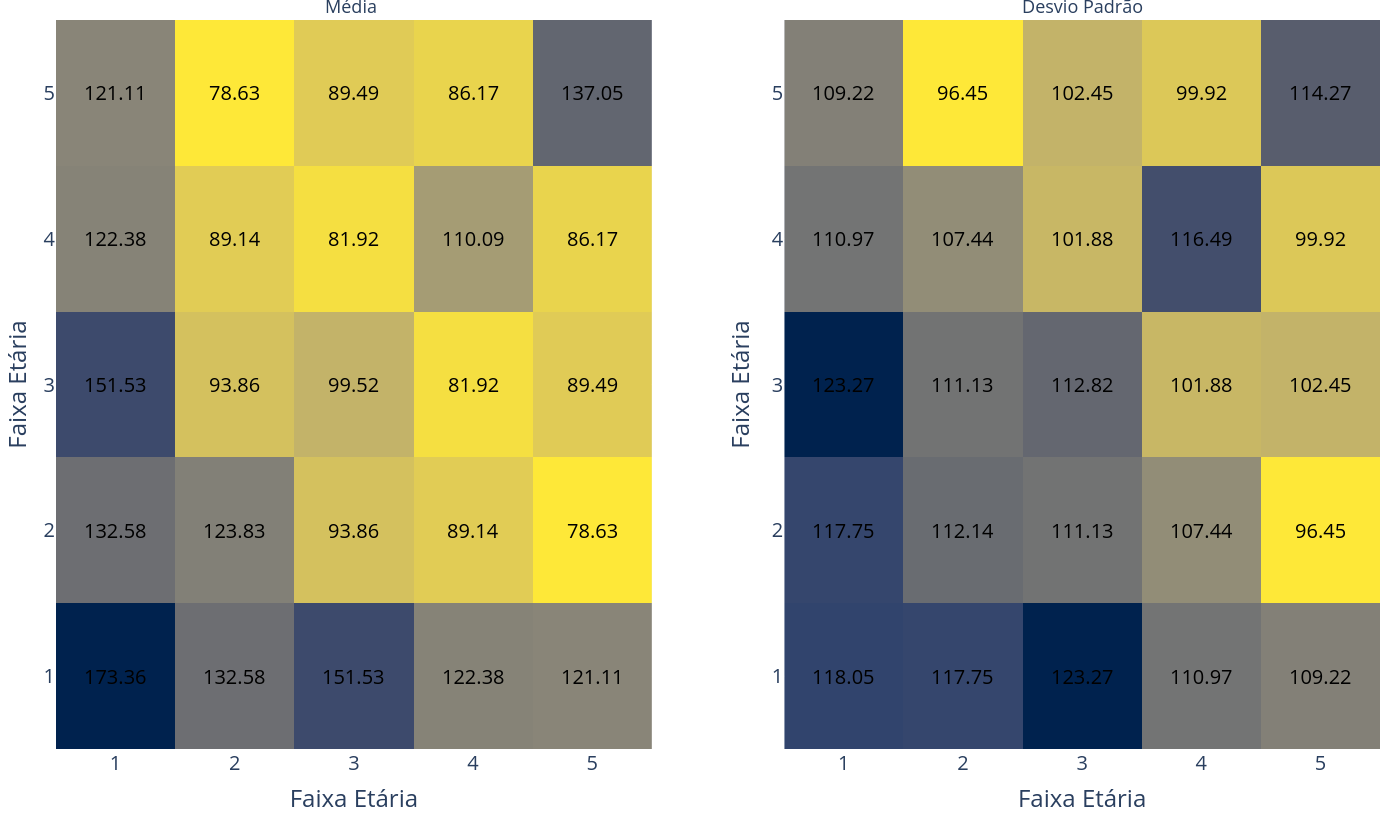
\includegraphics[scale= 0.35]{figuras/media_std.png}
    \captionsetup{font=small,justification=justified}
    \caption*{A imagem mostra a média e o desvio padrão do tempo de contato entre diferentes faixas etárias. A matriz da média indica que o contato é mais intenso dentro da mesma faixa etária e entre faixas etárias adjacentes, reduzindo conforme aumenta a diferença de idade. A matriz do desvio padrão mostra maior variação nos contatos dentro da mesma faixa e entre adjacentes, com menor variação entre faixas mais distantes. \\Fonte: Autor}
    \label{fig:mediastd}
\end{figure}

A matriz do desvio padrão indica que a variação no tempo de contato é mais significativa dentro da mesma faixa etária e com faixas etárias adjacentes, sugerindo maior inconstância nesses contatos. A Faixa Etária 1 apresenta o maior desvio padrão consigo mesma, seguido por desvios elevados com as Faixas Etárias 2 e 3, e menores com as Faixas Etárias 4 e 5. As Faixas Etárias 2 e 3 também exibem variações notáveis consigo mesmas e com faixas adjacentes, enquanto a Faixa Etária 4 tem maior variação com a Faixa Etária 5.

\subsection{Resultados da Rede gerada}

Os dados das Figuras \ref{fig:contatos_faixa} e \ref{fig:heat} foram utilizados como \textit{inputs} do Modelo de Configuração Ponderado, 

Especificamente, com os dados da Figura~\ref{fig:contatos_faixa} foi obtida a distribuição empírica do grau de cada nó de cada faixa etária e com os dados da Figura~\ref{fig:heat} foram estimados os parâmetros de uma distribuição multinomial para estabelecer quantas ligações vão para cada faixa etária. A partir disso e dado um valor de $p$ (parâmetro que aumenta o coeficiente de agrupamento) foi construída a rede para acontecer a simulação da epidemia. As características dessa rede são mostradas na Figura \ref{fig:regressao}
mostra-se como evolui o agrupamento com o incremento de $p$, que cresce com $C \propto p^{\alpha}$, tanto o agrupamento médio quanto o total no qual $\alpha_{medio } = 0.46$ e $\alpha_{total } = 0.55$. Após a aplicação do algoritmo foi recolhido os dados da rede e observou-se que para qualquer valor de $p$ a distribuição de graus tinha a mesma distribuição que a encontrada pela Figura \ref{fig:contatos_faixa} a partir do teste de Kolmogorov-Smirnov (Figura \ref{fig:comparacao}) \cite{manual}. Na Figura \ref{fig:modelo}
mostra-se a diferença absoluta ao final do algoritmo da proporção de conexões de cada faixa etária em comparação com a Figura \ref{fig:heat}, tendo uma diferença maior entre as conexões com faixa etária 1. Além disso na Figura \ref{fig:correlation} apresenta a correlação linear entre o Agrupamento e o Grau com o incremento de $p$, nele é possível notar que o valor decresce, ou seja nós com maior grau tendem a ter menos agrupamento, isso acontece, provavelmente, porque com grau muito alto existem muito mais combinações entre os sítios e o algoritmo não consegue contemplar esses nós com alto grau, expondo uma limitação do algoritmo.
\begin{figure}[H]
    \centering
    %PIF27092023
    \captionsetup{font=normalsize,skip=0.8pt,singlelinecheck=on,labelsep=endash}
    \caption{Agrupamento da rede em função de $p$}
    %PIF27092023 É possível apagar o enquadramento branco?        
    %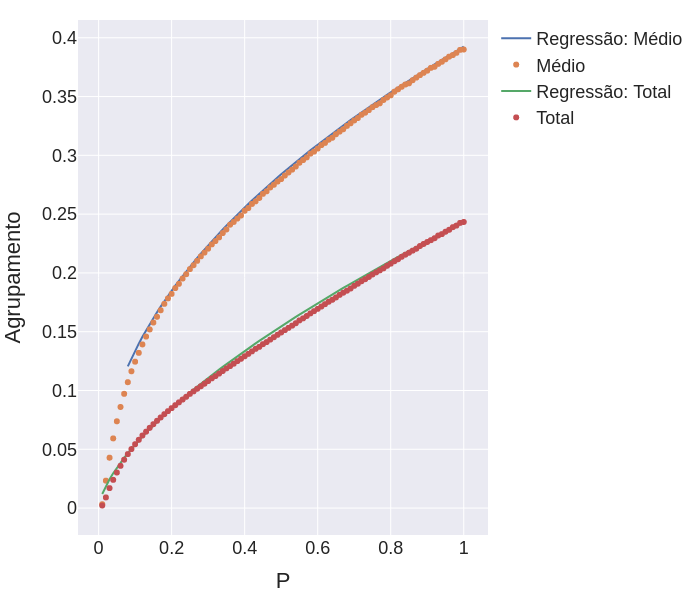
\includegraphics[scale= 0.5]{figuras/clustering_vs_p.png}
    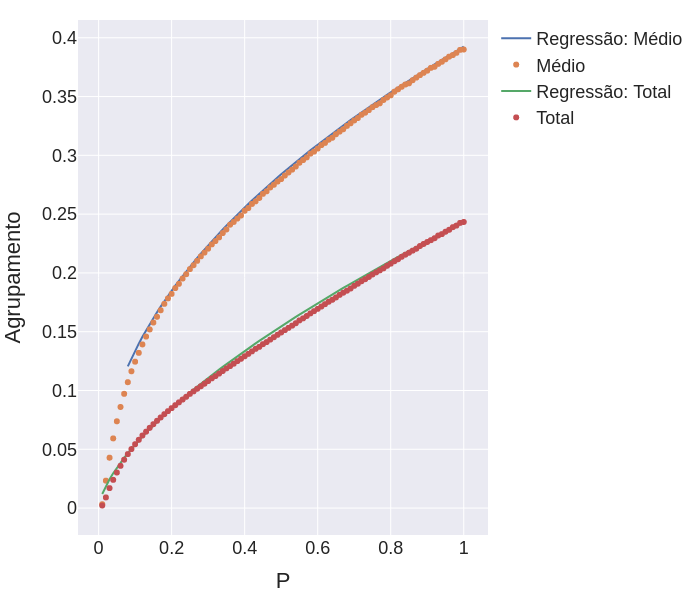
\includegraphics[scale= 0.6]{figuras/clustering_vs_p.png}
    \captionsetup{font=small,justification=justified}    \caption*{Evolução do agrupamento da rede em função 
    do incremento do valor de $p$, foi utilizada uma regressão linear para saber qual a função que rege encontrando $C \propto p^{\alpha}$.\\Fonte: Autor}
    \label{fig:regressao}
\end{figure}

\begin{figure}[H]
    \centering
    
    \captionsetup{font=normalsize,skip=0.8pt,singlelinecheck=on,labelsep=endash}
    \caption{Resultados da proporção de conexões entre faixas}
    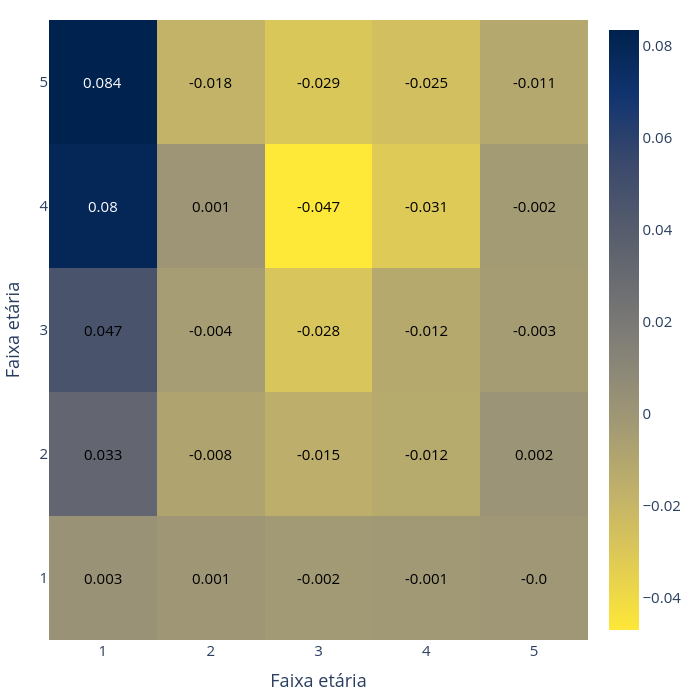
\includegraphics[scale= 0.4]{figuras/modelo.png}
    \captionsetup{font=small,justification=justified}
    \caption*{ A figura mostra a diferença absoluta entre a matriz de proporções de conexões entre as faixas etárias do modelo e do encontrado no POLYMOD essa diferença se mantém constante independe do valor de $p$.}
    \label{fig:modelo}
\end{figure}
\begin{figure}[H]
    \centering
    \captionsetup{font=normalsize,skip=0.8pt,singlelinecheck=on,labelsep=endash}
    \caption{Distribuição de Graus $p = 1.0$}
    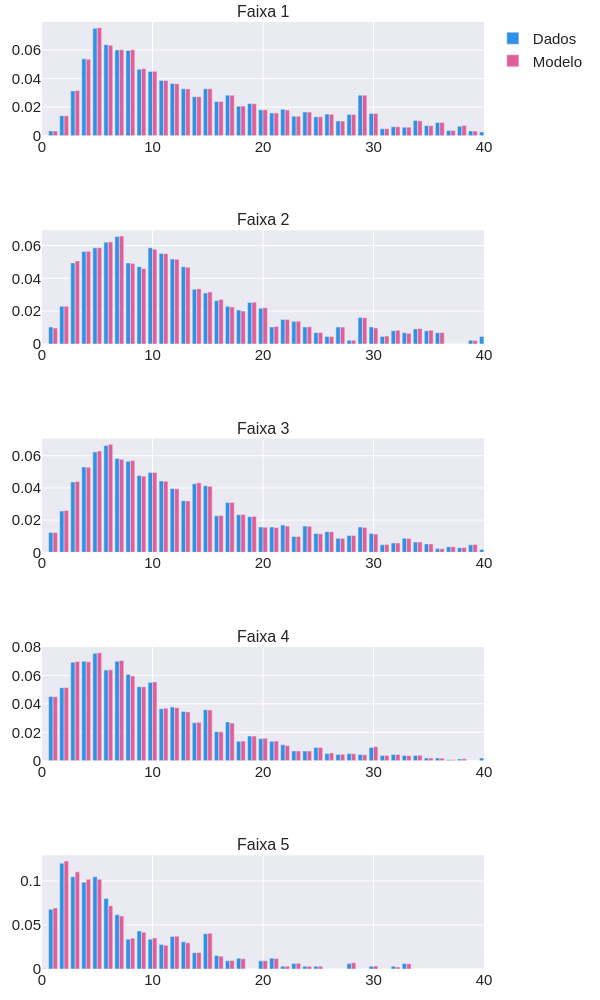
\includegraphics[scale= 0.4]{figuras/comparacao.png}
    \captionsetup{font=small,justification=justified}
    \caption*{Comparação de como fica a distribuição de graus comparando modelo com $p = 1.0$ com dados do POLYMOD, é possível ver todas as faixas foram bem no teste de comparação.\\Fonte: Autor}
    \label{fig:comparacao}
\end{figure}

\begin{figure}[H]
    \centering
    \captionsetup{font=normalsize,skip=0.8pt,singlelinecheck=on,labelsep=endash}
    \caption{Agrupamento da rede em função de $p$}
    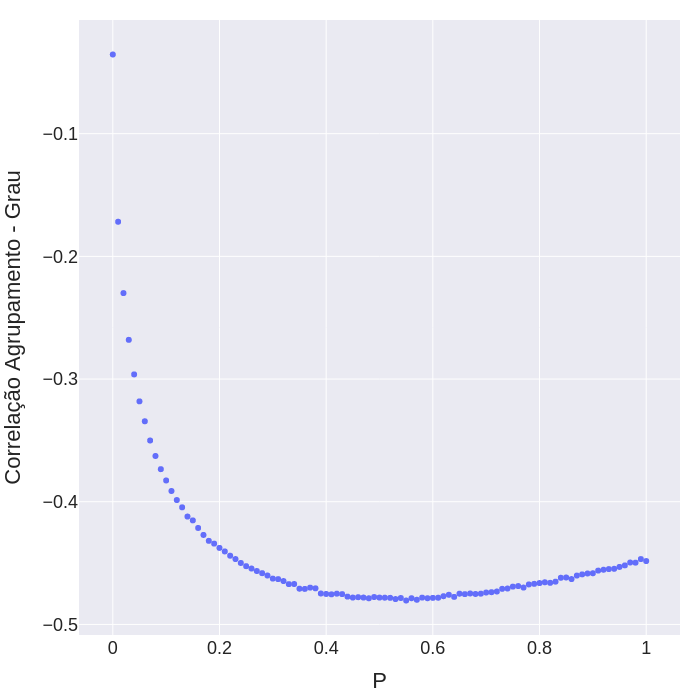
\includegraphics[scale= 0.5]{figuras/correlation.png}
    \captionsetup{font=small,justification=justified}    \caption*{Evolução do agrupamento da rede em função 
    do incremento do valor de $p$, foi utilizada uma regressão linear para saber qual a função que rege encontrando $C \propto p^{\alpha}$.\\Fonte: Autor}
    \label{fig:correlation}
\end{figure}

\subsection{Resultados do Modelo de Infecção}

Em suma o modelo utilizado é o Modelo de Configuração Ponderado usando como entrada uma distribuição de graus empírica, a distribuição de faixas etárias brasileira e a distribuição de ligações entre faixas etárias encontradas no banco de dados do POLYMOD, no caso da infecção os parâmetros são os que foram encontrados na literatura ou calculados pelo OpenDataSUS, além disso com o POLYMOD foram calculados as médias e desvios do tempo de contato entre os indivíduos que serão considerados. A simulação acontece do dia 0 até o dia 465 iniciando com 10 nós infectados — para garantir que a simulação não termine cedo — no compartimento Exposto e todos os outros sítios como Suscetíveis. A vacinação ocorre no dia 100, nesse dia são aplicadas vacinas para uma fração $f$ da rede para sítios no compartimento Suscetível,Exposto , Recuperado ou Assintomático dado um critério de prioridade que é determinado pelo valor das centralidades introduzidas anteriormente. Se o indivíduo não estiver apto a ser vacinado no dia e após todos os aptos serem vacinados ainda existirem vacinas sobrando, então se ele atingir um dos compartimentos aptos ele será vacinado.

Para as centralidades que dependem da ponderação nos nós foram utilizadas a probabilidade do nó ser assintomático e a probabilidade dele morrer, para centralidades que originalmente não utilizam ponderação dos nós, apenas nas arestas utilizamos a seguinte mudança:
\begin{equation}
    Z_{\nu,\mu} = w_{\nu,\mu}\cdot(\Theta_\nu + \Theta_\mu).
\end{equation}
O valor de $\Theta_\nu$ e $\Theta_\mu$ e das centralidades com ponderação dos nós será feito de duas abordagens diferentes: Altruísta e a Individualista. A Altruísta será calculando as centralidade pensando que o nó $\nu$ a ser calculado esteja tentando infectar as outras pessoas na rede e matar elas, na abordagem Individualista as centralidades são calculadas pensando no nó $\nu$ sendo infectado por todas as outras pessoas na rede e morrer.

Após a implementação do modelo epidemiológico no modelo de redes escolhidos foram escolhidos pela performasse do algoritmo que após o dia 100 a infecção estabilizava e esse seria o dia da vacinação, deste modo simula-se a situação real na qual a vacina só se tornou disponível após a COVID-19 já ter se espalhado por todo o mundo. Anteriormente a esse dia a rede se comporta, para $p = 0$ (com agrupamento médio de 0.01), de acordo com as Figuras \ref{fig:pre_vacina} e \ref{fig:pre_vacina_mortos}. A Figura \ref{fig:pre_vacina} mostra a evolução da epidemia, em que pode-se observar que a proporção de indivíduos suscetíveis diminui rapidamente até o dia 25, que é o tempo de incubação, para posteriormente aumentar e atingir um estado de estabilidade. A fração de indivíduos infectados (a soma da fração de assintomáticos com a de sintomáticos) aumenta até atingir um pico, com  30\% da população total sendo infectada simultaneamente, seguido por um declínio. Finalmente, a fração de indivíduos recuperados aumenta até que 58\% da população esteja nesse estado, estabilizando posteriormente. Já a Figura \ref{fig:pre_vacina_mortos} mostra a evolução  da  fração de mortos e a fração de hospitalizados, nesse sentido observa-se que o número máximo de hospitalizados observado foi cerca de 0.46\% da rede, enquanto o número de mortos cresce indefinidamente. Neste trabalho, não consideramos a capacidade do sistema hospitalar, pois neste caso, precisaríamos de informações sobre a taxa de recuperação e de morte de sintomáticos que precisariam ser internados e não foram por falta de leitos que não são facilmente determinadas.   

\begin{figure}[H]
    \centering
    \captionsetup{font=normalsize,skip=0.8pt,singlelinecheck=on,labelsep=endash}
    \caption{Fração de Suscetíveis, Infectados e Recuperados antes da aplicação de qualquer estratégia de vacinação}
    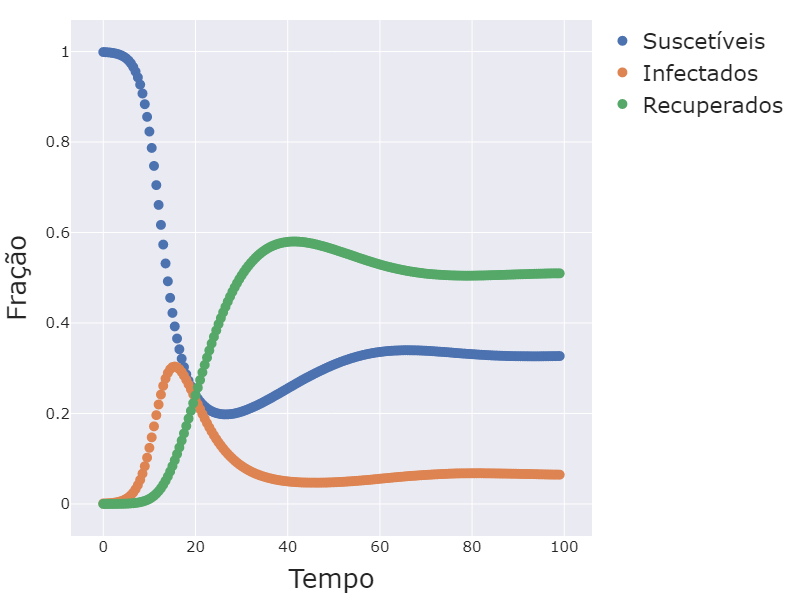
\includegraphics[scale= 0.5]{figuras/pre_vacina_nponderado.png}
    \captionsetup{font=small,justification=justified}
    \caption*{Resultados antes da aplicação de qualquer 
    estratégia de vacinação para uma rede $N$ = 10000 com $p $ = 0 após 1000 realizações. Inicialmente, a proporção de suscetíveis diminui rapidamente, seguida por um aumento e estabilização. A fração de infectados atinge um pico, afetando 
    40\% da população, e depois diminui. Paralelamente, a proporção de recuperados aumenta e estabiliza em 71\% da população.}
    \label{fig:pre_vacina}
\end{figure}

\begin{figure}[H]
    \centering
    \captionsetup{font=normalsize,skip=0.8pt,singlelinecheck=on,labelsep=endash}
    \caption{Fração de Hospitalizados e Mortos antes da aplicação de qualquer estratégia de vacinação}
    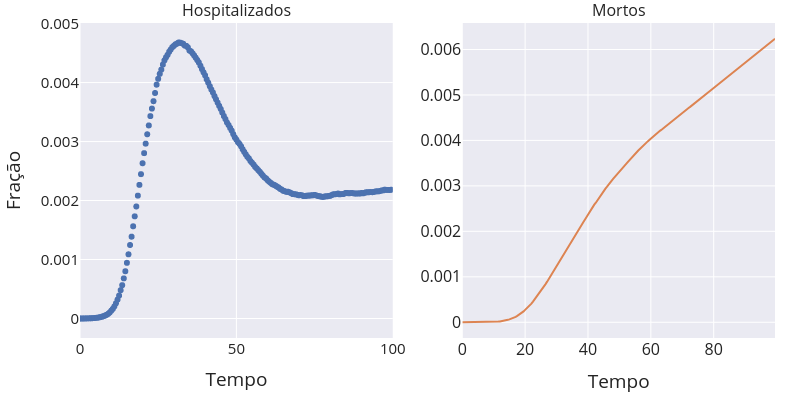
\includegraphics[scale= 0.5]{figuras/pre_vacina_mortos_nponderado.png}
    %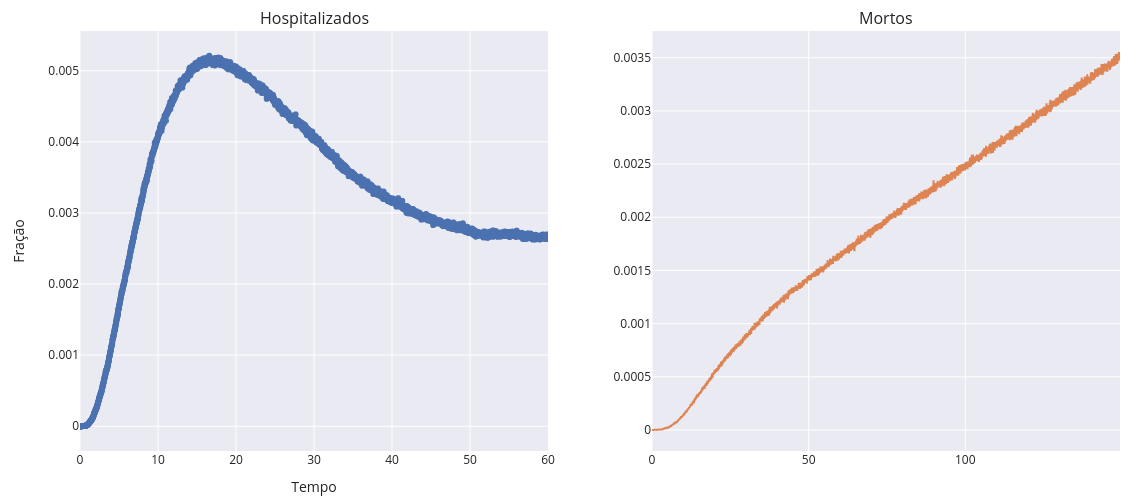
\includegraphics[scale= 0.4]{figuras/pre_vacina_mortos-PIF.png}
    \captionsetup{font=small,justification=justified}
    \caption*{Simulações foram feitas para uma rede $N$ = 2028 com $p $ = 0 após 1000 realizações.}
    \label{fig:pre_vacina_mortos}
\end{figure}

Com o aumento de $p$ surgem diferenças com o comportamento da infecção, a Figura mostra \ref{fig:pre_vacina_mortos_p} que a rede tem uma quantidade menor de mortos, contudo a infecção demora mais para crescer, decair e estabilizar, ou seja o agente permanece mais tempo na rede, isso se deve, provavelmente, ao fato de que em média os idosos tem conexões menores e sabemos anteriormente que o MCP aumenta o agrupamento de nós com poucas conexões e que os mais idosos tem mais conexões com os mais novos pois precisam de cuidados e esses têm pouca chance de morrer mas tem mais conexões, portanto o que deve acontecer é que a infecção se espalha mais no grupo dos mais jovens.

\begin{figure}[H]
    \centering
    \captionsetup{font=normalsize,skip=0.8pt,singlelinecheck=on,labelsep=endash}
    \caption{Fração de Mortos e Hospitalizados antes da aplicação de qualquer estratégia de vacinação e diferentes valores de $p$}
    \vspace{5pt}
    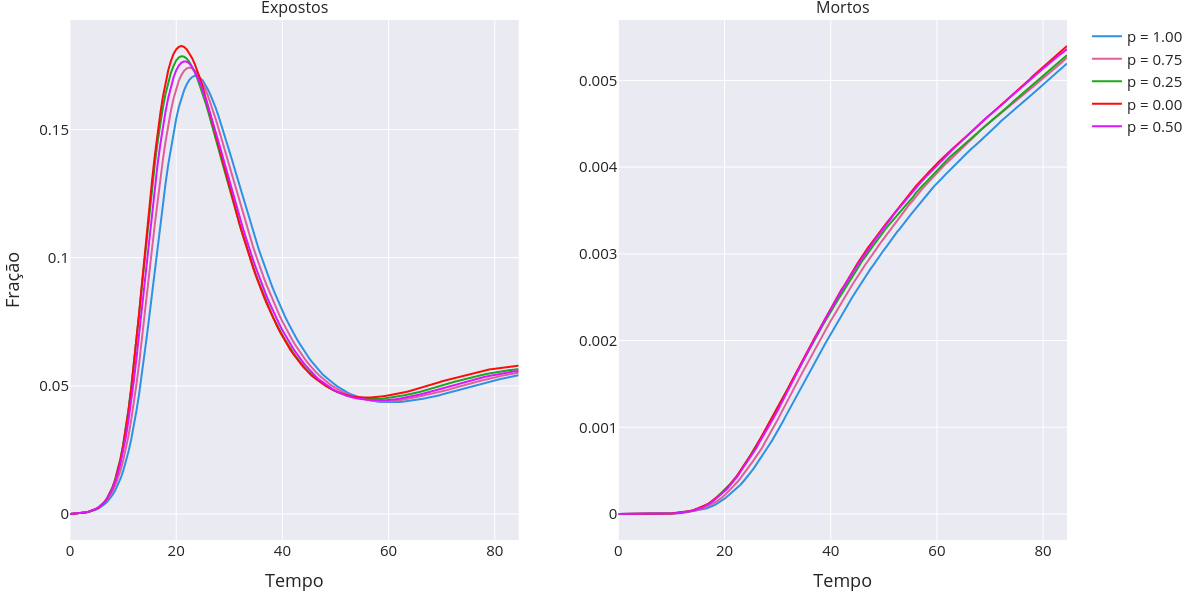
\includegraphics[width=\textwidth]{figuras/pre_vacina_mortos_p_nponderado.png}
    \captionsetup{font=small,justification=justified}
    \caption*{Resultados para fração de Mortos e Hospitalizados e função do tempo antes da aplicação de qualquer estratégia de vacinação para uma rede $N$ = 2028 para valores de $p$ = 0, $p$ = 0.5 e $p$ = 1.}
    \label{fig:pre_vacina_mortos_p}
\end{figure}

Para finalizar, fizemos a comparação entre como a rede se espalha nos primeiros 100 dias no caso ponderado e não ponderado nesse caso  não houve uma diferença significativa entre o avanço da infecção, a Figura \ref{fig:compara_ponderado_nponderado} mostra para Expostos que a diferença é pouco perceptível isso é visível para qualquer compartimento da rede. Apesar disso será feita a análise das centralidades comparando caso ponderado e não ponderado, porém no caso da infecção pré-vacina não há diferença o que acarreta numa simplificação do modelo o que favorece o tempo computacional dos algoritmos.

\begin{figure}[H]
    \centering
    \captionsetup{font=normalsize,skip=0.8pt,singlelinecheck=on,labelsep=endash}
    \caption{Fração de Infectados com diferentes estratégias de vacinação e $p$ = 0.0}
    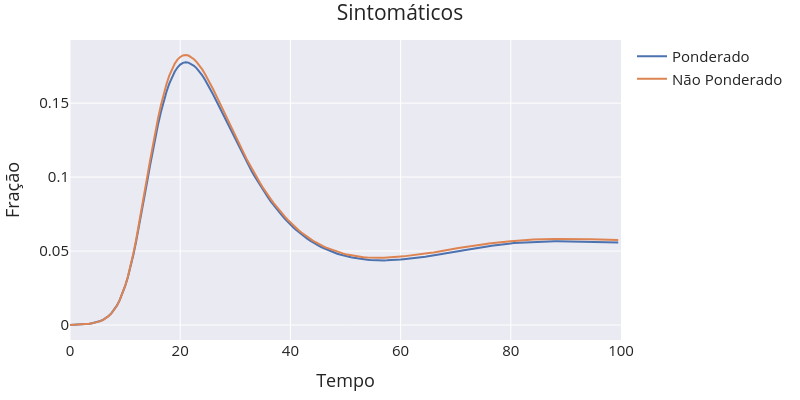
\includegraphics[scale= 0.5]{figuras/compara_ponderado_nponderado.png}
    \captionsetup{font=small,justification=justified}
    
    \caption*{ Após 60 dias, diferentes estratégias de vacinação foram aplicadas, mostrando variação no número de infectados. As estratégias de priorização de graus e centralidade de intermediação foram mais eficazes em conter a proliferação, enquanto as estratégias baseadas em idade e aleatória foram as menos eficazes, apresentando desempenho quase equivalente. As demais estratégias, com exceção da centralidade excêntrica, mostraram comportamento semelhante.}
    \label{fig:compara_ponderado_nponderado}
\end{figure}

Após os 100 dias, foi aplicado a vacina com diversas estratégias seguindo as centralidades em redes apresentadas anteriormente. Ao final foram coletadas o tempo total hospitalizado $T_H$, a fração de mortos $F_M$ e fração de indivíduos necessária para extinguir a doença $F_I$. Assim para cada parâmetro foi feito um \textit{ranking} mostrando para as melhores centralidades, para $T_H$ e $F_M$ foi integrado a área do gráfico de parâmetro \textit{versus} $f$. Para determinar qual centralidade apresentou o melhor desempenho geral, calculou-se a média dos respectivos valores de cada centralidade para cada parâmetro avaliado. A qualidade de cada centralidade é varia perante a rede, ou seja, com a alteração de $p$ o \textit{ranking} será diferente e poderá existir diferentes melhores estratégias, seria então necessário estimar os valores de $p$ da rede real para saber qual seria a melhor estratégia. 

A Figura \ref{fig:resultados_metricas} para o caso sem ponderação compara como ficaram os resultados para $p = 0$ e $p = 1$ mostrando 4 métricas, o caso aleatório, idade, a melhor na métrica e a melhor na média, quando o gráfico apresenta apenas 3 curvas significa que a melhor na métrica é a mesma para melhor na média. Esse esquema será repetido na Figura \ref{fig:resultados_metricas_ponderado}, optamos por motivo de muitas centralidades terem sido testadas - 29 para caso não ponderado e 65 para caso não ponderado - para ver os resultados de todas as métricas consulte o Anexo 1.

É possível perceber que em todas as métricas e mudando o valor de $p$ a idade não foi uma boa estratégia no geral contra a doença, um resultado importante é que para extinguir a doença seria necessário vacinar cerca de 80\% da população, entretanto na melhor estratégia foram necessários apenas 32\% para extinguir a doença. Porém é notável que para uma fração menor de 15\% da rede vacinada a idade foi muito boa em comparação às melhores, entretanto ela foi pior para valores maiores. Essa comparação é feita pois foi a principal estratégia utilizada pelos governos.

\begin{figure}[H]
    \centering
    \captionsetup{font=normalsize,skip=0.8pt,singlelinecheck=on,labelsep=endash}
    \caption{Fração de Infectados com diferentes estratégias de vacinação e $p$ = 0.0}
    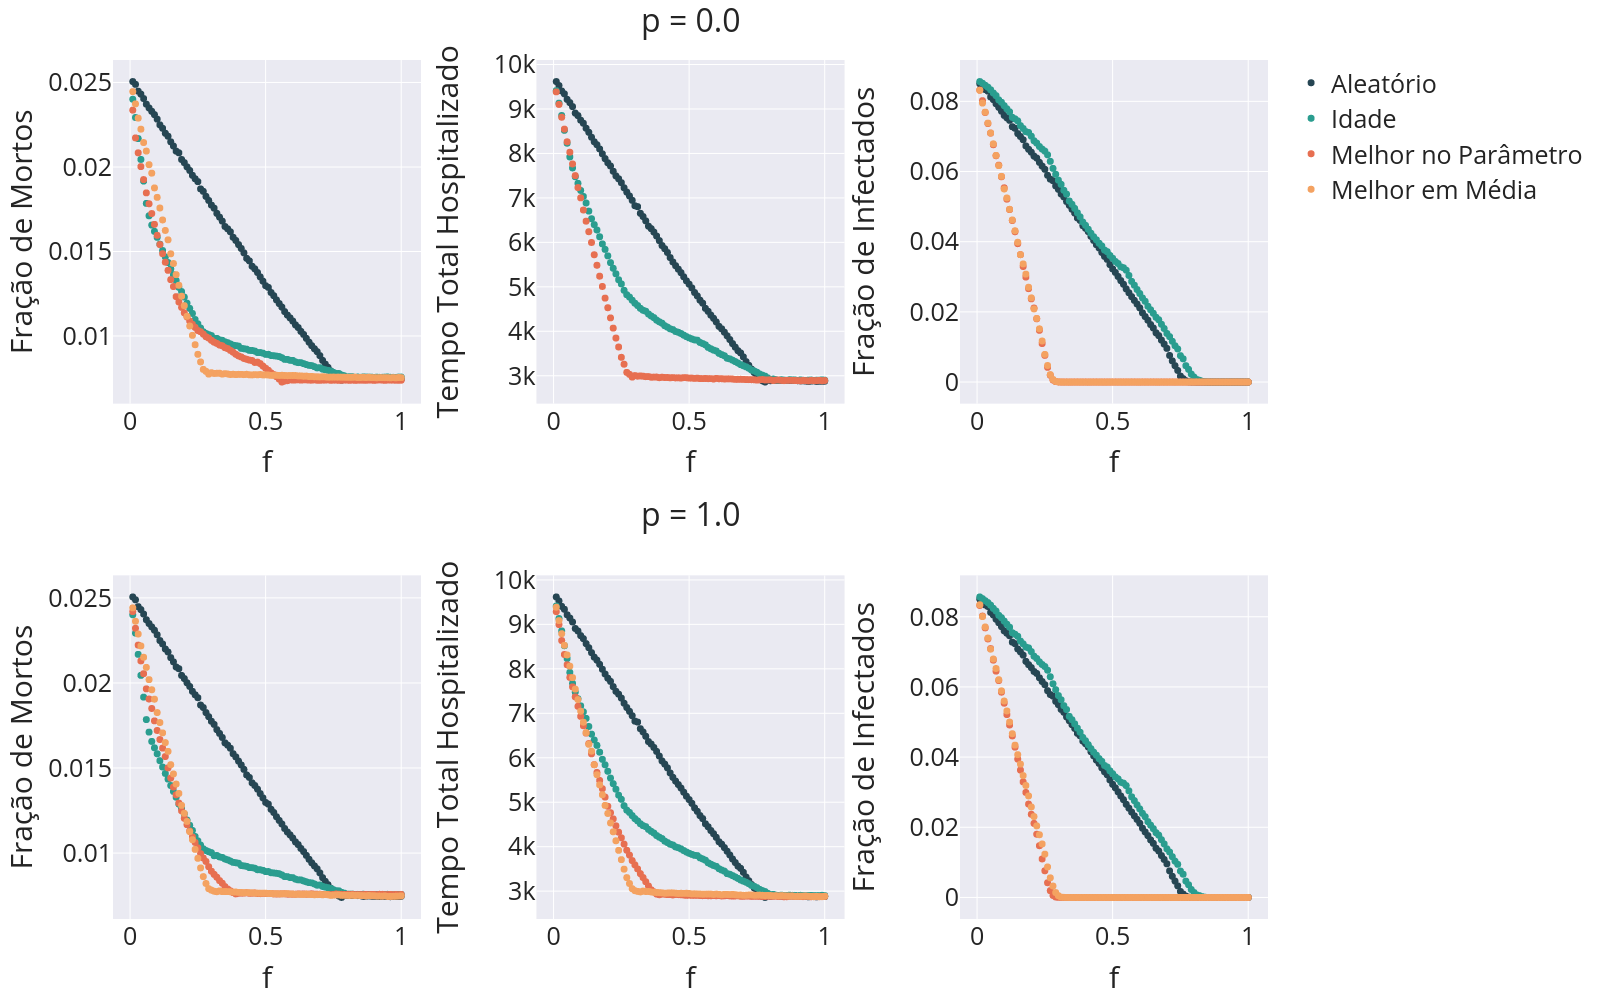
\includegraphics[scale= 0.3]{figuras/cmpara_p_f.png}
    \captionsetup{font=small,justification=justified}
    
    \caption*{ Após 60 dias, diferentes estratégias de vacinação foram aplicadas, mostrando variação no número de infectados. As estratégias de priorização de graus e centralidade de intermediação foram mais eficazes em conter a proliferação, enquanto as estratégias baseadas em idade e aleatória foram as menos eficazes, apresentando desempenho quase equivalente. As demais estratégias, com exceção da centralidade excêntrica, mostraram comportamento semelhante.}
    \label{fig:resultados_metricas}
\end{figure}

\begin{figure}[H]
    \centering
    \captionsetup{font=normalsize,skip=0.8pt,singlelinecheck=on,labelsep=endash}
    \caption{Fração de Infectados com diferentes estratégias de vacinação e $p$ = 0.0}
    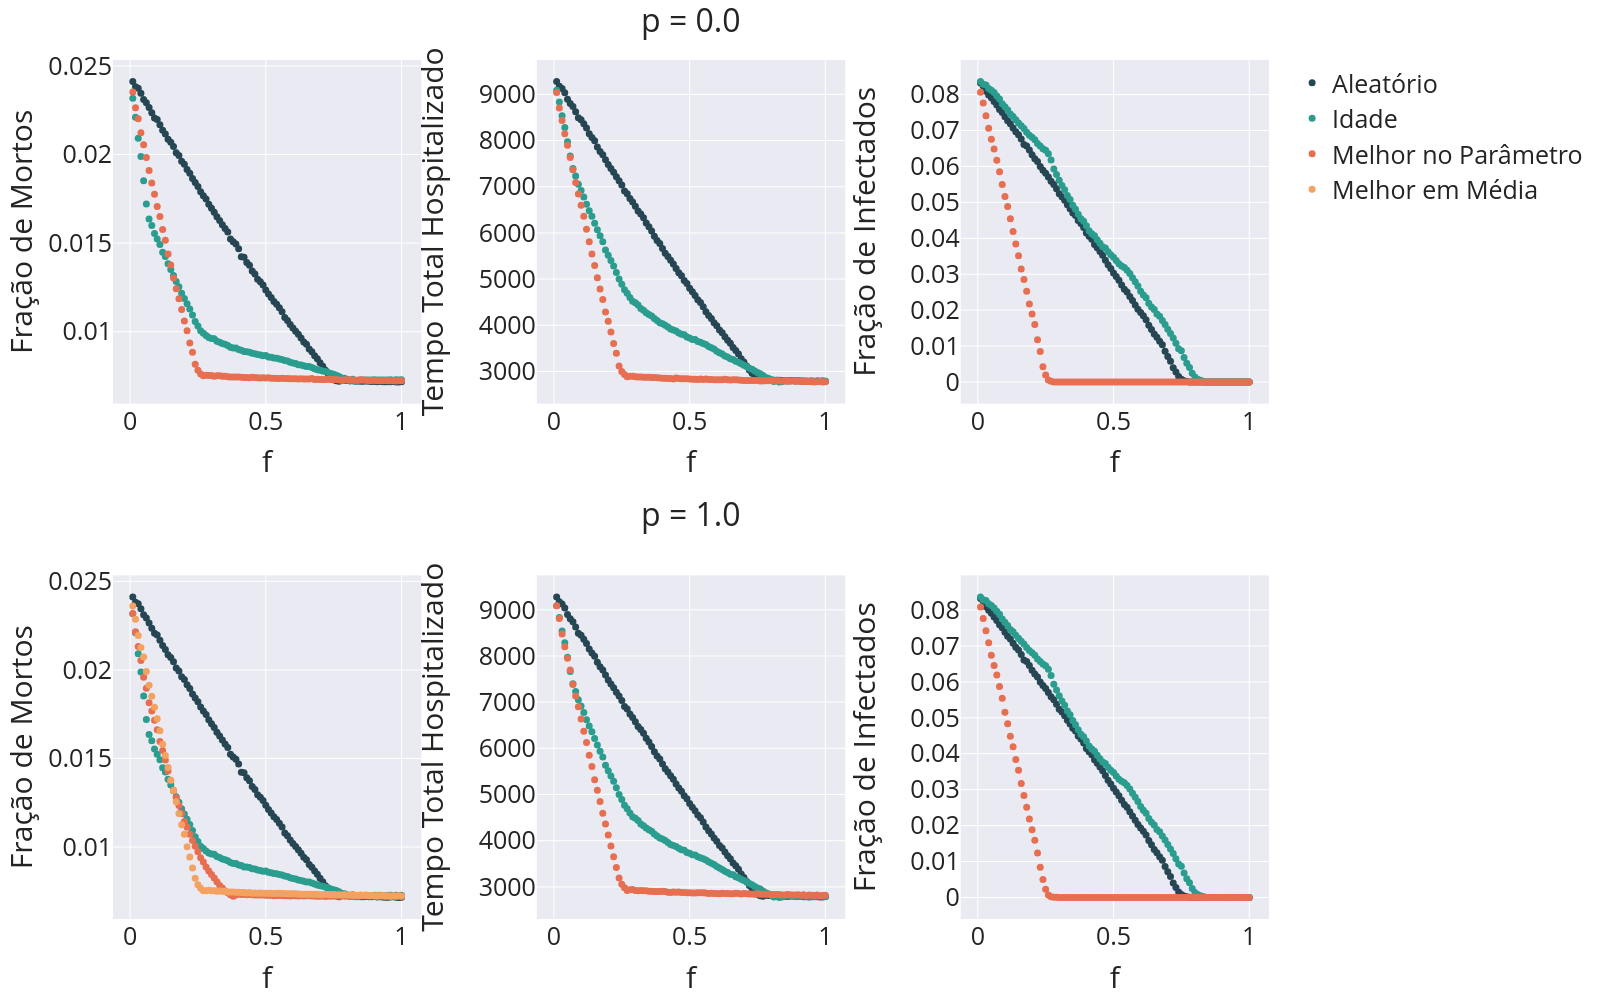
\includegraphics[scale= 0.3]{figuras/newplot.png}

    \captionsetup{font=small,justification=justified}
    
    \caption*{ Após 60 dias, diferentes estratégias de vacinação foram aplicadas, mostrando variação no número de infectados. As estratégias de priorização de graus e centralidade de intermediação foram mais eficazes em conter a proliferação, enquanto as estratégias baseadas em idade e aleatória foram as menos eficazes, apresentando desempenho quase equivalente. As demais estratégias, com exceção da centralidade excêntrica, mostraram comportamento semelhante.}
    \label{fig:resultados_metricas_ponderado}
\end{figure}

Embora os gráficos forneçam uma indicação preliminar da diferença entre a melhor estratégia em termos de um determinado parâmetro e o desempenho médio, é fundamental realizar uma avaliação para determinar se existe uma diferença significativa entre as métricas, nesse caso foi optado por dado os valores de cada centralidade em cada métrica foi calculado a integral da sua respectiva curva e foi feito a correlação de Spearman entre as métricas. A Figura \ref{fig:Spearman} mostram o valor da correlação para diferentes valores de $p$ para o caso não ponderado e ponderado. É possível ver que as duas métricas mais distintas entre si são $F_M$ e $F_I$ mostrando que a métrica que foca em diminuir a mortalidade uma não necessariamente previne a espalhamento da doença, outrossim com o incremento de $p$ $F_M$ e $T_H$ se tornam mais próximas, por fim existe uma diferença no caso ponderado, na qual as métricas são mais próximas entre si, principalmente a $F_M$ e $T_H$ o que poderia ser descartada nesse caso.

\begin{figure}[H]
    \centering
    \captionsetup{font=normalsize,skip=0.8pt,singlelinecheck=on,labelsep=endash}
    \caption{Fração de Infectados com diferentes estratégias de vacinação e $p$ = 0.0}
    
    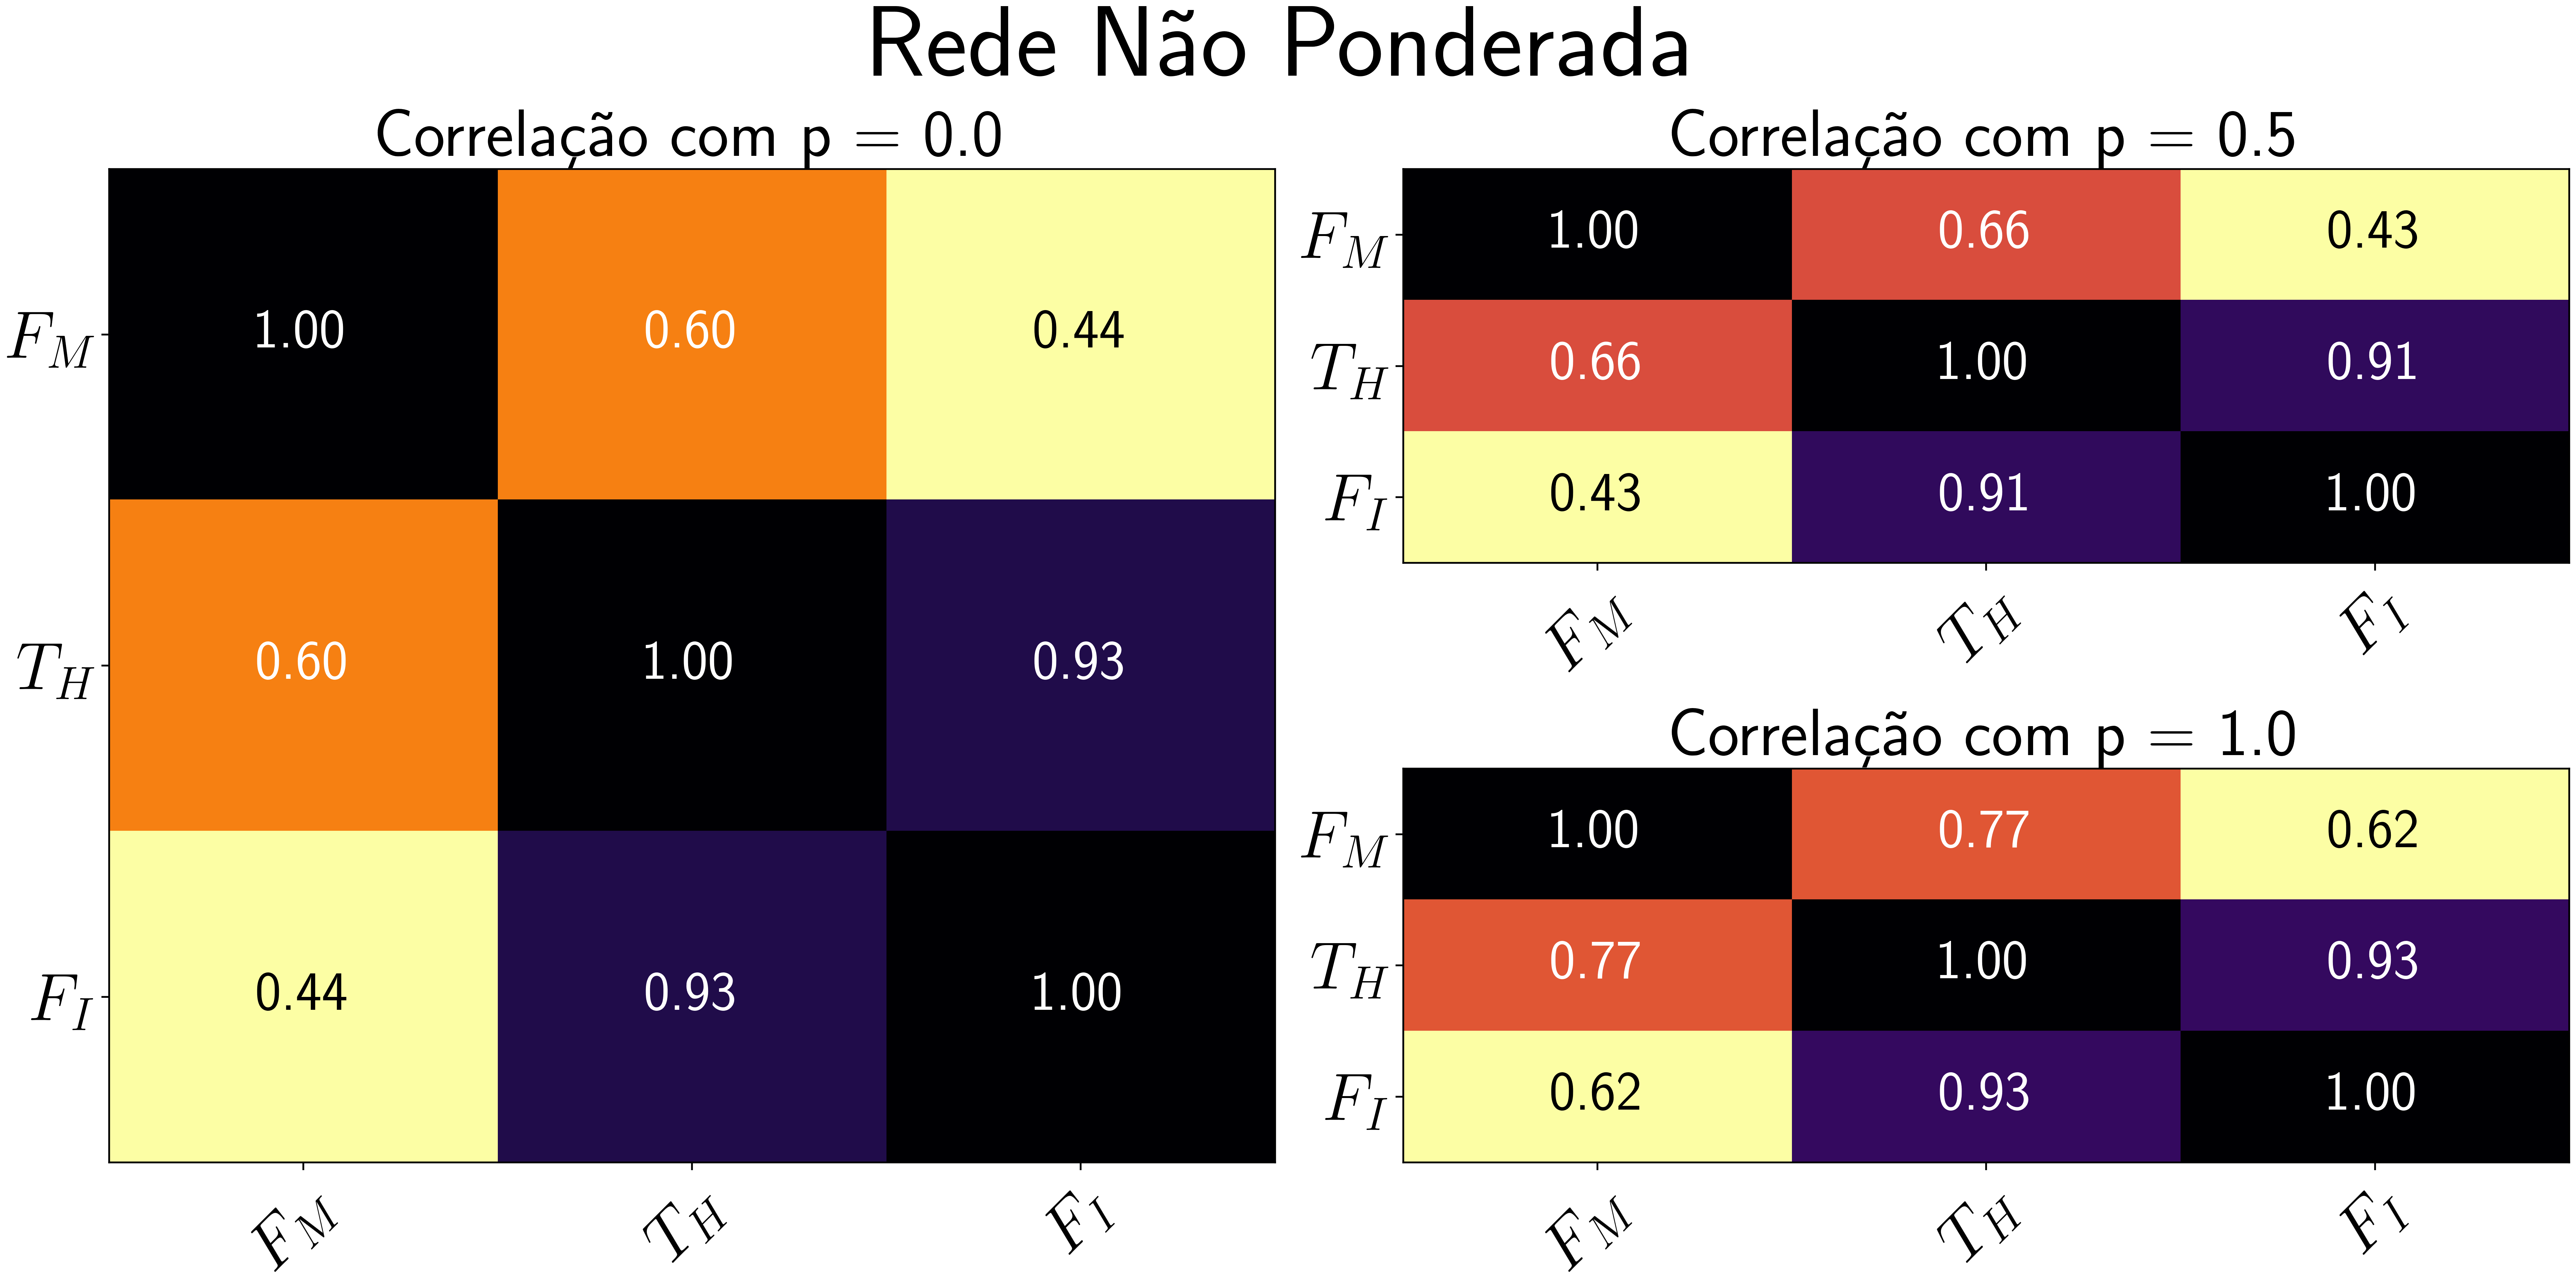
\includegraphics[scale= 0.4]{figuras/corr_p.png}
    \\
    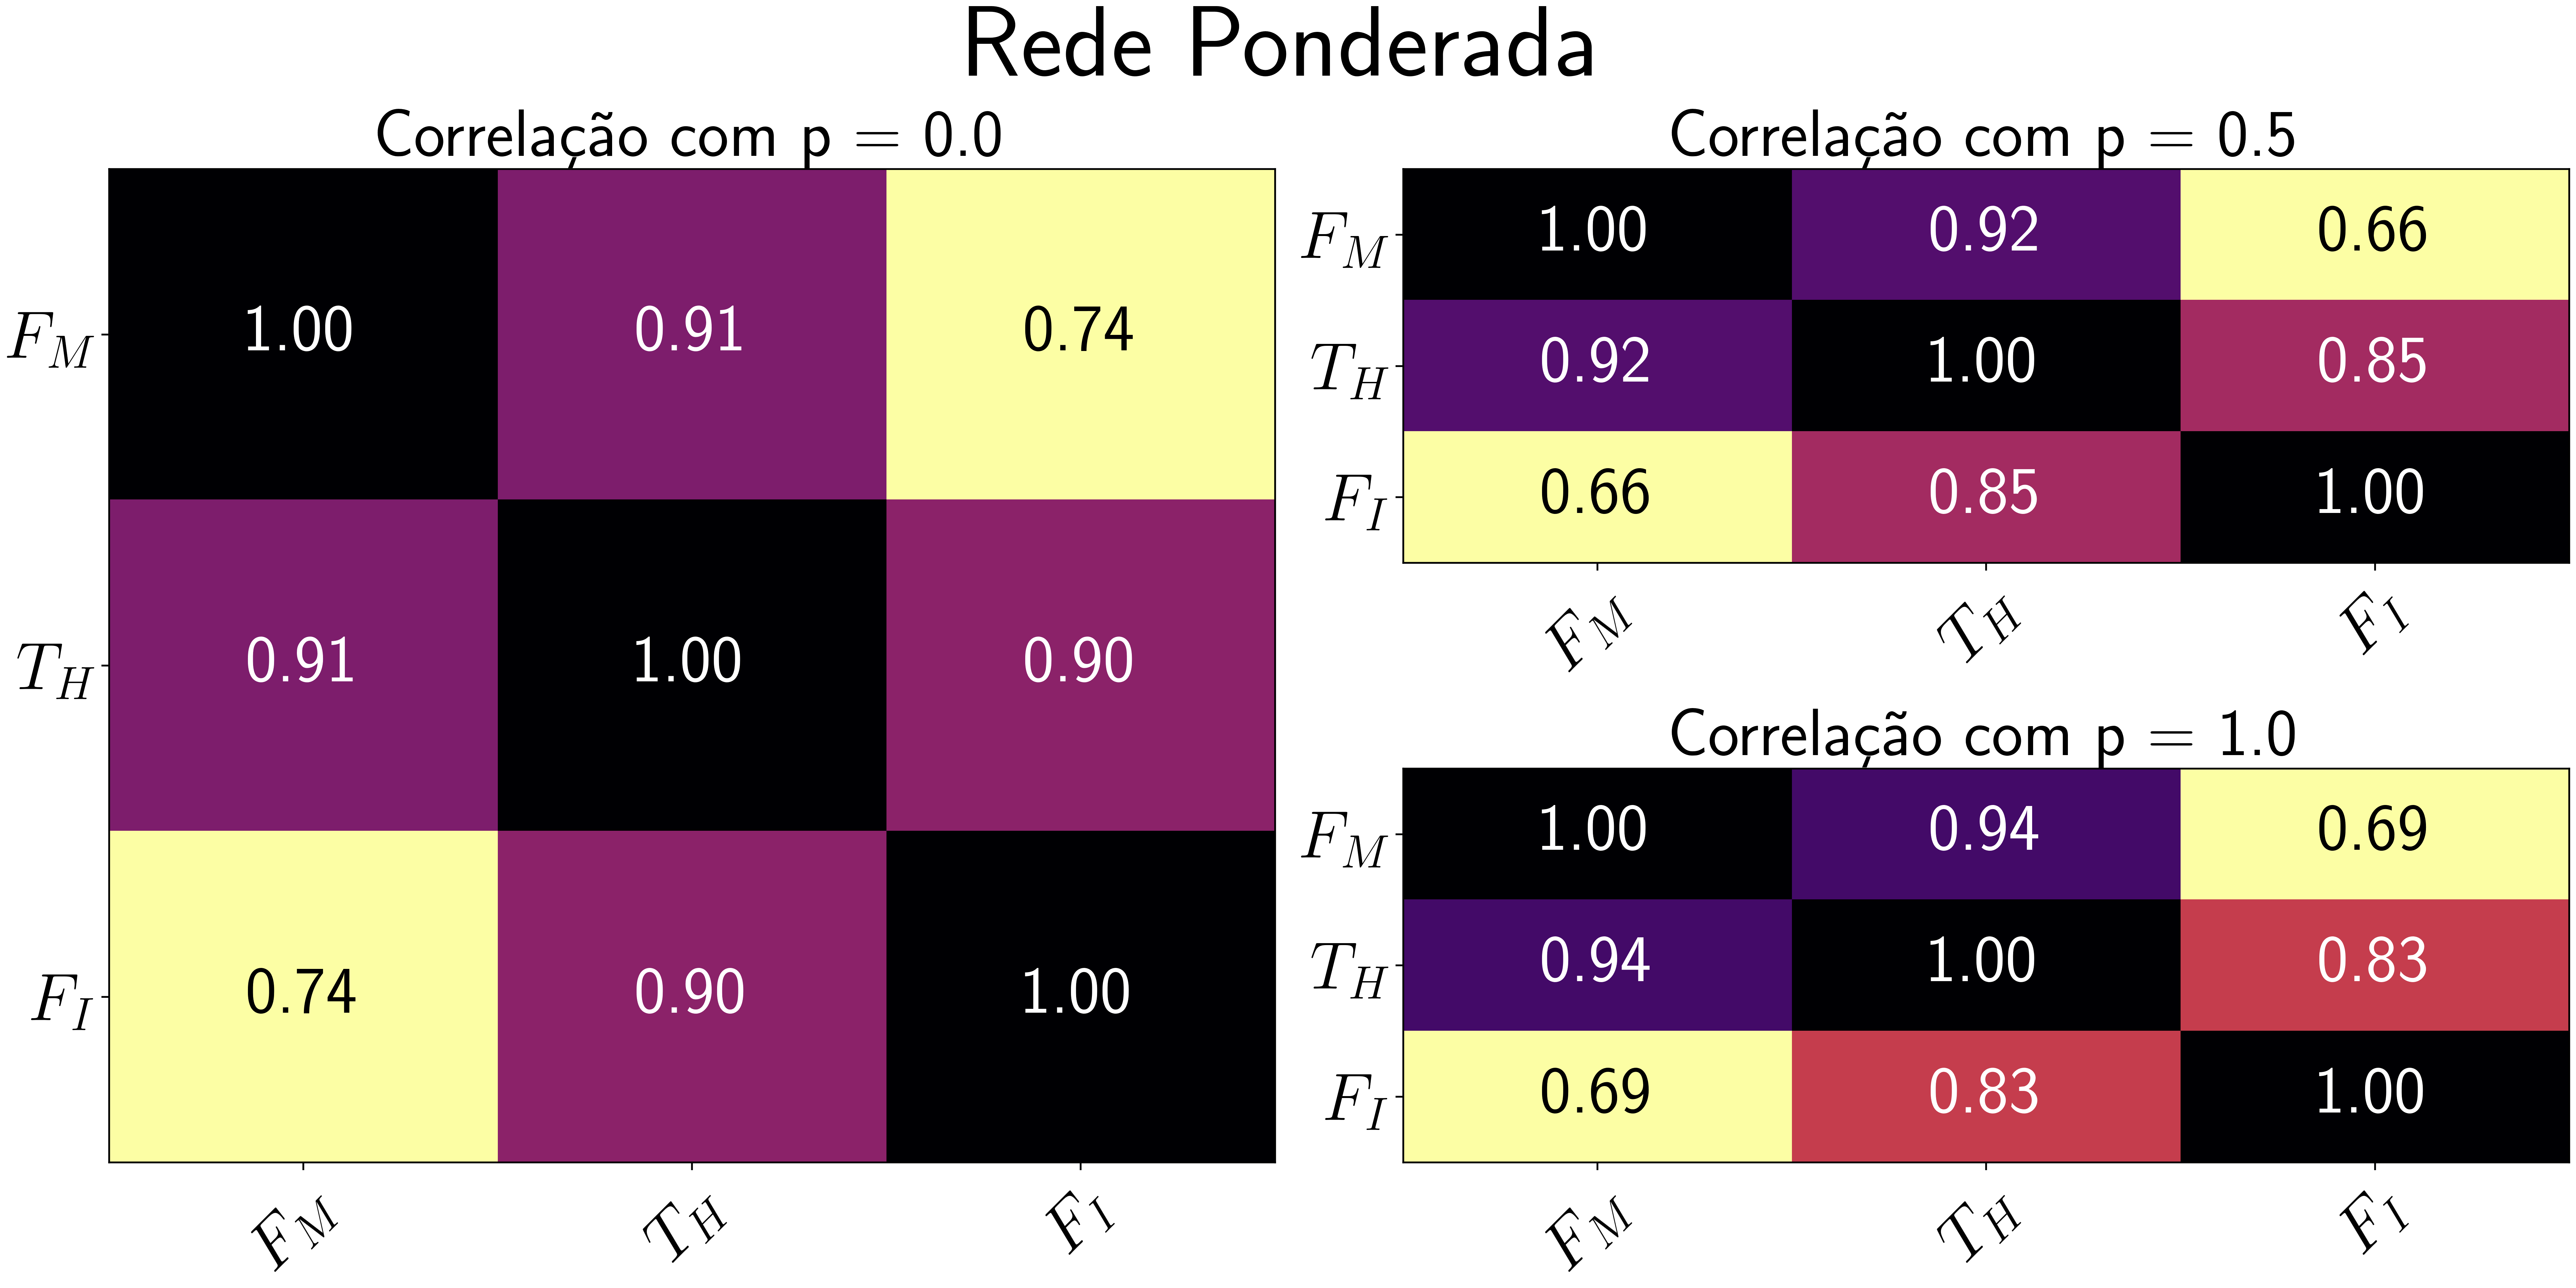
\includegraphics[scale= 0.4]{figuras/corr_p_ponderado.png}
    \captionsetup{font=small,justification=justified}
    \caption*{}
    \label{fig:Spearman}
\end{figure}

Como mostrado pela Figura \ref{fig:Spearman} as relações entre métricas mudam com o incremento de $p$, assim o próprio \textit{ranking} muda com a variação do parâmetro, assim a Figura \ref{fig:Spearman_p} mostra a correlação de Spearman do \textit{ranking} para cada par de $p$ para rede não ponderada e ponderada, é possível ver que para o caso não ponderado no geral existe uma alta correlação entre os pares, contudo para $F_M$ os valores são menores do que para a $F_I$ e aquele apresenta valores são mais correlacionados com agrupamentos maiores do que este. A conclusão é que no geral o posicionamento das estratégias é bastante estável com o aumento do agrupamento tanto no caso ponderado quanto não ponderado. Isso é bastante útil pois não foi medido o agrupamento da rede real de contatos entre pessoas e com essa estabilidade não se torna tão necessário estimar esse valor.

\begin{figure}[H]
    \centering
    \captionsetup{font=normalsize,skip=0.8pt,singlelinecheck=on,labelsep=endash}
    \caption{Fração de Infectados com diferentes estratégias de vacinação e $p$ = 0.0}
    
    \includegraphics[scale= 0.4]{figuras/compara_agrupamento_nponderado.png}
    \\
    \includegraphics[scale= 0.4]{figuras/compara_agrupamento_ponderado.png}
    \captionsetup{font=small,justification=justified}
    \caption*{}
    \label{fig:Spearman_p}
\end{figure}

Anteriormente foram apresentadas as centralidades e as suas versões utilizando ponderamento nas arestas, contudo a utilização da forma ponderada tem um custo computacional bastante considerável, portanto foi avaliado como a métrica foi em comparação com a sua versão ponderada considerando a diferença relativa entre o valor na métrica com ponderação em relação ao valor sem considerar ponderação. A Figura \ref{fig:compara_pesos} mostra como ficou a comparação para dois casos de agrupamento $p = 0$ e pode se perceber que várias métricas não foram bem com o incremento da ponderação nas arestas, principalmente a Utilidade que para $F_I$ teve uma perca de 100\%, mas algumas conseguiram se beneficiar, mas no geral teve um saldo pior.

\begin{figure}[H]
    \centering
    \captionsetup{font=normalsize,skip=0.8pt,singlelinecheck=on,labelsep=endash}
    \caption{Fração de Infectados com diferentes estratégias de vacinação e $p$ = 0.0}
    
    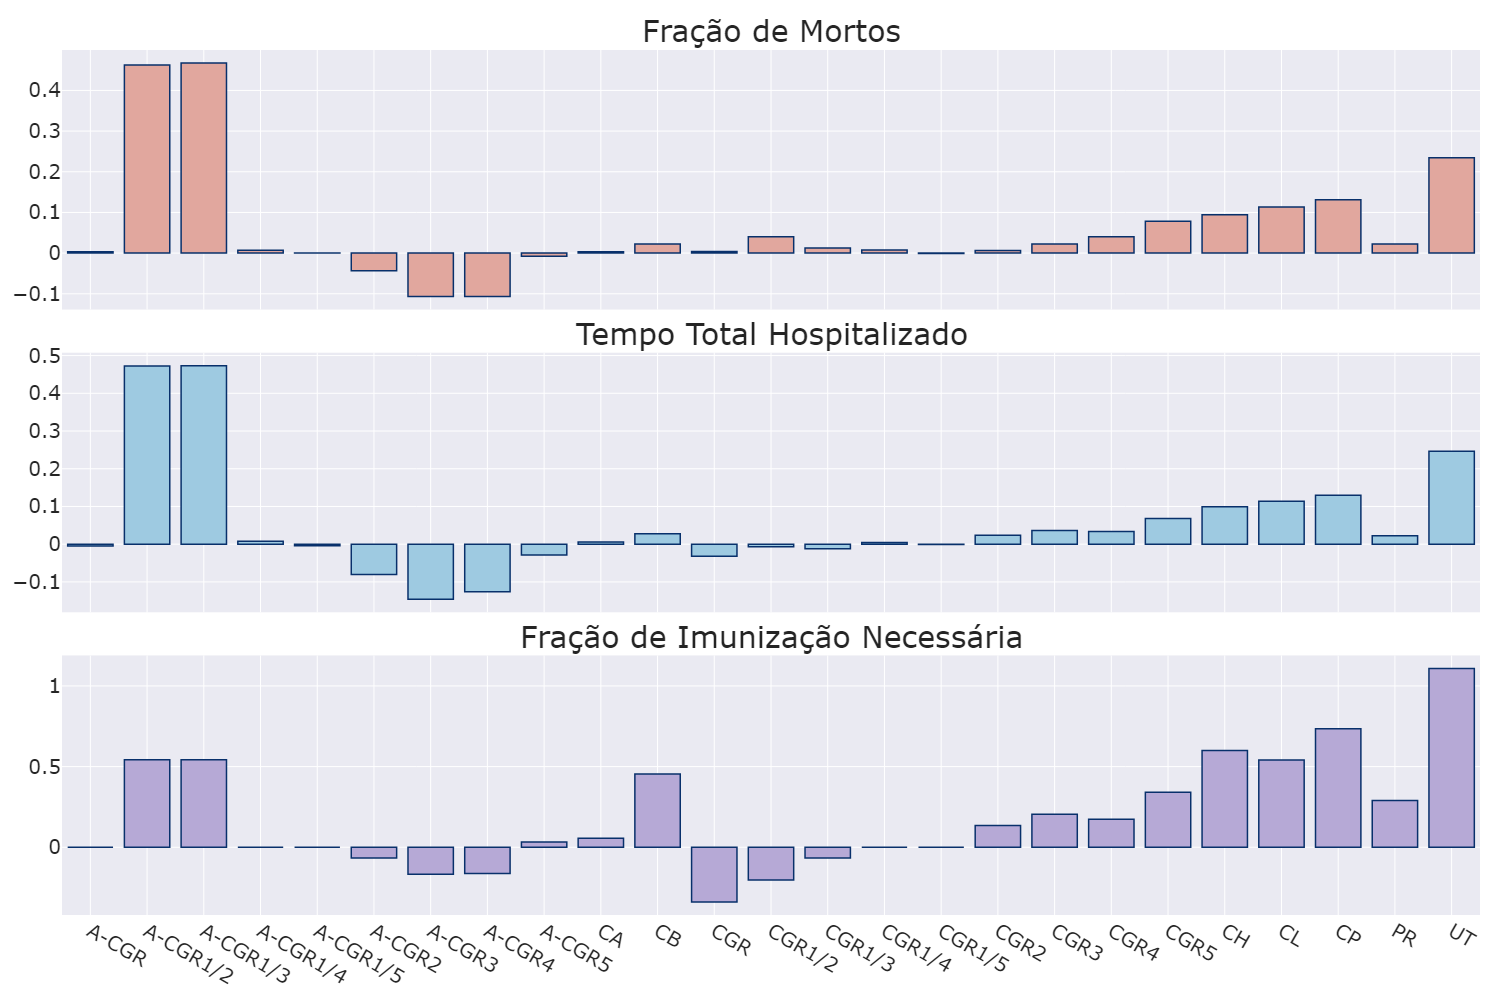
\includegraphics[scale= 0.3]{figuras/compara_pesos_0.0.png}
    \\
    \captionsetup{font=small,justification=justified}
    \caption*{}
    \label{fig:compara_pesos}
\end{figure}

Diferente da comparação entre o ponderado e não ponderado, a comparação entre Individualista e Altruísta pelo erro relativo é consenso, como mostra a Figura \ref{fig:compara_altruismo}, que o Individualista foi muito pior que a abordagem Altruísta pois ou os valores eram bastante parecidos ou havia uma piora muito grande, no caso da rede ponderada muitas métricas pioraram e nas outras havia pouca mudança já na rede não ponderada houve o contrário.

\begin{figure}[H]
    \centering
    \captionsetup{font=normalsize,skip=0.8pt,singlelinecheck=on,labelsep=endash}
    \caption{Fração de Infectados com diferentes estratégias de vacinação e $p$ = 0.0}
    
    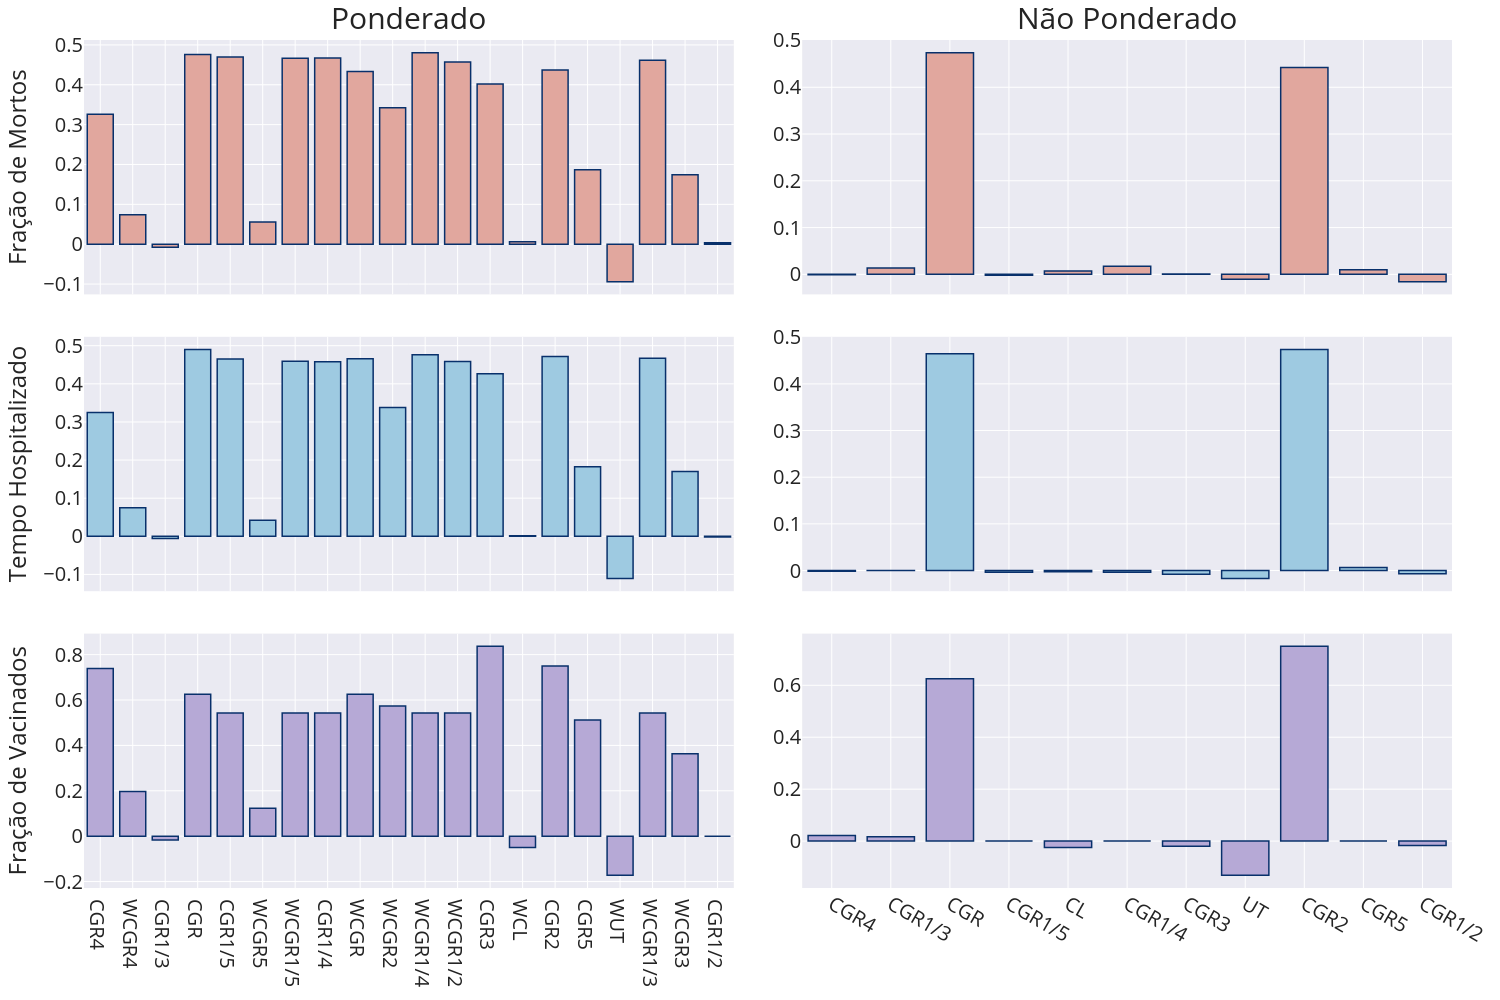
\includegraphics[scale= 0.3]{figuras/compara_altruismo_0.0.png}
    \\
    \captionsetup{font=small,justification=justified}
    \caption*{}
    \label{fig:compara_altruismo}
\end{figure}
	%\chapter{Conclusões e Trabalhos Futuros}
\label{chap:conclusoes-e-trabalhos-futuros}

Neste trabalho, foram investigados diferentes métricas de centralidade e quais delas são melhores efetivas em identificar indivíduos chave na propagação do COVID-19. Ao estudar uma pesquisa conseguimos obter dados que nos ajudaram a construir um modelo de redes, apesar da pesquisa não contribuir para isso, propomos um modelo de formação de rede a partir de uma sequência de graus e as conexões entre indivíduos de faixa etária diferentes e propomos um modelo de propagação do COVID-19 e vacinação na rede.

%Resultados 

%Próximos passos
Entretanto, essa pesquisa ainda apresenta limitações, o POLYMOD apesar de obter vários dados não se sabe a abrangência total e até que ponto se pode aplicar para diferentes países e culturas, o MCP não consegue aumentar o agrupamento para nós com grau maiores, não se sabe se é uma limitação do algoritmo, dos dados, ou é um comportamento padrão, o modelo epidemiológico que foi proposto abre margem para o estudo de superlotação de hospitais que foi uma característica importante na pandemia. Essas são uma das várias limitações do trabalho e propostas para futuras pesquisas nessa área.
	
	%Elementos pós-textuais	
	\bibliography{3-pos-textuais/referencias}
%	\imprimirglossario %	
	%\imprimirapendices
		% Adicione aqui os apendices do seu trabalho
		%\apendice{EXEMPLO DE APÊNDICE}
\label{ap:A}

Um apêndice é um documento elaborado pelo autor, diferentemente do anexo. Geralmente, se coloca como apêndice, questionários, códigos de programação, tabelas que tomariam muito espaço no meio do trabalho.
		%\apendice{ Questionário utilizado para}
\label{ap:B}

\begin{questao}
	\item Esta é a primeira questão com alguns itens:
		\begin{enumerate}
			\item Este é o primeiro item
			\item Segundo item
		\end{enumerate}
	\item Esta é a segunda questão:
		\begin{enumerate}
			\item Este é o primeiro item
			\item Segundo item
		\end{enumerate}
	\item Lorem ipsum dolor sit amet, consectetur adipiscing elit. Nunc dictum sed tortor nec viverra. consectetur adipiscing elit. Nunc dictum sed tortor nec viverra.
		\begin{enumerate}
			\item consectetur
			\item adipiscing
			\item Nunc
			\item dictum
		\end{enumerate}
\end{questao}

		%\apendice{ Códigos-fontes utilizados para}
\label{ap:C}

\lstinputlisting[language=C++,caption={Hello World em C++}]{figuras/main.cpp}


\begin{lstlisting}[language=Java,caption={Hello World em Java}]
public class HelloWorld {
	public static void main(String[] args) {
		System.out.println("Hello World!");
	}
}
\end{lstlisting}


		
		%\imprimiranexos
		% Adicione aqui os anexos do seu trabalho
		%\anexo{ Exemplo de um anexo}
\label{an:ex_anexo_a}

Um anexo é um documento que não foi elaborado pelo autor, ou seja, o autor apenas anexa. Anexos podem ser tabelas, mapas, diagramas, \textit{datasheets}, manuais e etc. 




		%\anexo{ Exemplo de um anexo em PDF}
\label{an:ex_anexo_b}

O autor pode anexar um \gls{PDF}, traduzido como formato portátil de documento. Veja o código fonte utilizado para anexar o arquivo ``Sikasil.pdf'' que foi colocado dentro da pasta ``anexos'' que por sua vez está dentro da pasta ``elementos-pos-textuais''. Tenha muita atenção na hora de especificar o local do arquivo. Recomenda-se não utilizar caracteres especiais para nomear pastas e, principalmente, arquivos. 

Pode-se fazer uma descrição sucinta do arquivo anexado.

%Comando para incluir um arquivo em PDF:
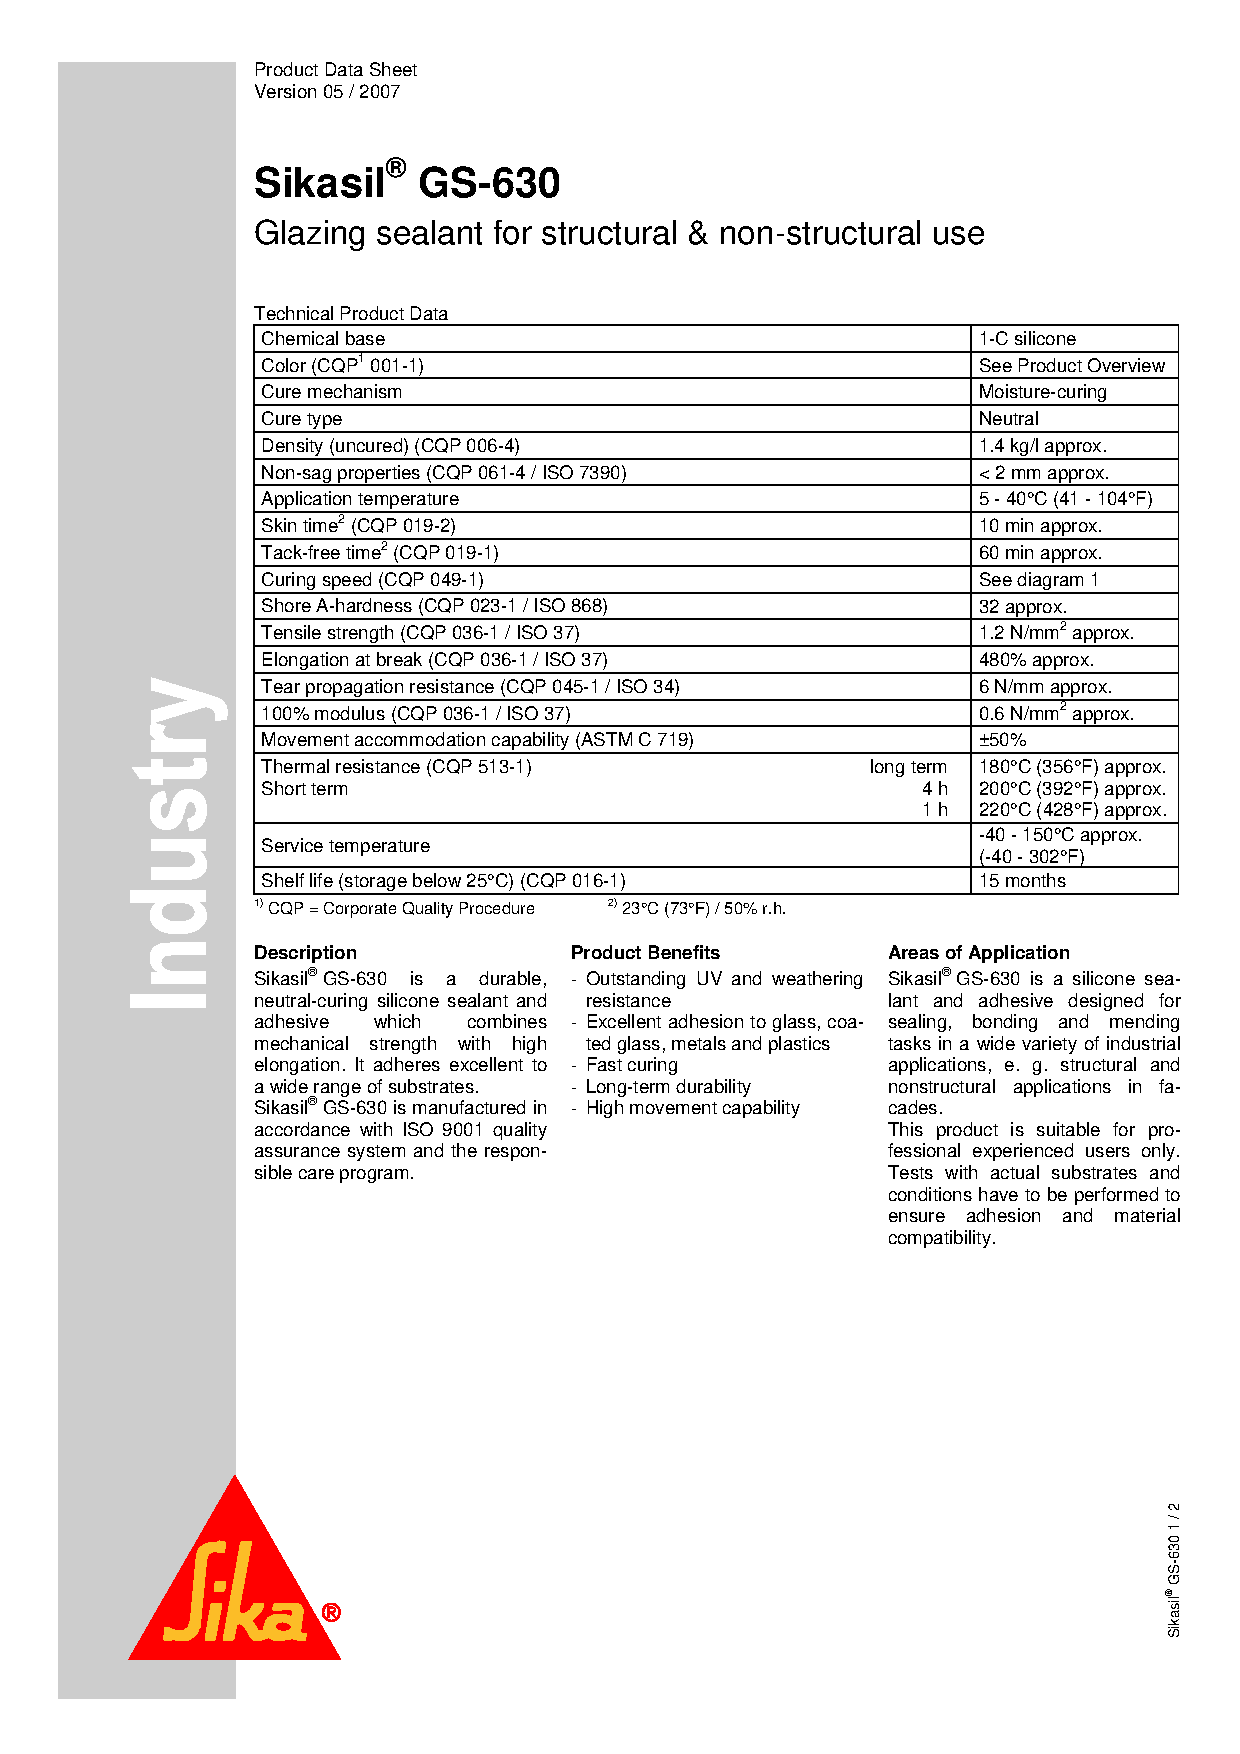
\includepdf[pages={-}]{3-pos-textuais/anexos/Sikasil.pdf}

		
    %\imprimirindice
    
	

\end{document}